%% ------------------------------------------------------------------------- %%
\chapter{Música no som digitalizado} %Nome do capítulo.
\label{cap:resultados} %Rótulo para futura referência ao capítulo. Em qualquer lugar da tese, você poderá citar este capítulo através de ~\ref{cap:introducao}. Você escolhe o argumento de \label e pode ser qualquer coisa (Ex: \label{Procedimento_Experimental})
\begin{quotation}
\small
'The increasing dominance of graphic interfaces for music software obscured 
the continuing presence of the command-line tradition, 
the code writer, the hacker. The code writing of deferred time 
computer programming may be assembled out of time order, debugged and optimized.'

\emph{Simon Emmerson, Living electronic music.\cite{Emmerson}}
\end{quotation}


\section{Caracterização da nota musical em tempo discreto}\label{sec:notaDisc}
Em diversos contextos artísticos e teóricos, 
a música é pensada através de 
unidades chamadas notas e 
estas unidades compreendidas como "átomos" constituintes da música.\cite{Wisnick, Lovelock, Webern}
Atualmente, estas notas
são tidas como um paradigma de proposta musical
e, de um ponto de vista cognitivo, como discretizações
que facilitam e enriquecem o fluxo de informação através da música.\cite{Roederer, Lacerda}
Canonicamente, as notas possuem ao menos duração, volume, altura e timbre.\cite{Lacerda} Estas
são qualidades tratáveis quantitativamente.\cite{Roederer}
Assim, as características da nota musical digital básica são dadas pelas amostras igualmente espaçadas no tempo
da onda mecânica que representam (veja seção~\ref{sec:audio} sobre áudio PCM).

Todas as relações desta seção estão no Apêndice~\ref{sec:cod1}, as montagens musicais \emph{Quadros sonoros} e \emph{Reduced-fi} estão nos Apêndices~\ref{ap:quadros} e~\ref{ap:reduced}. Estas implementações estão também disponíveis online como parte do \emph{toolbox} \massa.\cite{MASSA}

\subsection{Duração}
A frequência (ou taxa) de amostragem $f_a$ 
é definida como o número de amostras por segundo. Seja
a sequência $T_i=\{t_i\}$ um conjunto ordenado de amostras reais separadas por $\delta_a=1/f_a$ segundos.
Uma nota musical de duração $\Delta$
se apresenta como uma sequência de $ \lfloor \Delta . f_a \rfloor $ amostras\footnote{O
limite superior de uma sequência é um número natural, mas $ \Delta . f_a $
só satisfaz esta condição em casos muito excepcionais. É necessário
escolher um inteiro próximo de $\Delta . f_a$ e admitir algum erro. Por simplicidade, será considerada sempre a parte inteira da multiplicação, descrita por $\lfloor \Delta . f_a \rfloor$ e aceito o erro de até $-\delta_a$ segundos. Por exemplo, $\delta_a=1/44100 \approx 2,3.10^{-5}$, por volta de 23 microssegundos, o que é razoável para usos musicais.}:

\begin{equation}\label{eq:dur}
T_{i}^{\Delta}={\{t_i\}}_{i=0}^{\lfloor \Delta . f_a \rfloor -1}
\end{equation}

Seja $\Lambda = \lfloor \Delta . f_a \rfloor$ o número de amostras da sequência, de forma que $T_i=\{t_i\}_0^{\Lambda-1}$.

\subsection{Volume}
A sensação de volume sonoro depende da reverberação e distribuição dos harmônicos, dentre outras características trabalhadas na seção~\ref{varInternas}. Pode-se obter variações do volume através da potência da onda~\cite{Chowning}:

\begin{equation}\label{eq:potencia}
pot(T_i)=\frac{\sum_{i=0}^{\Lambda -1} t_i^2}{\Lambda}
\end{equation} 

O volume final dependerá sempre da amplificação do sinal nos alto-falantes, assim o crucial é a potência relativa de uma nota em relação às outras ou de um trecho da música em relação ao resto. As diferenças de volume são medidas em decibels, e estes são
calculados diretamente com as amplitudes através das energias ou potências\footnote{Lembrando que, devido à percepção logarítmica,
em um som de volume $v$ a redução da potência $p$ para uma mesma fração $\nu . p $ 
com $\nu \in [0,1]$ é sentido como a mesma diminuição $\kappa$ do volume $v-\kappa$ com $\kappa \geq 0$.}:

\begin{equation}\label{decibels}
V_{dB}=10log_{10}\frac{pot(T^{'}_i)}{pot(T_i)}
\end{equation}

A quantidade $V_{dB}$ possui a unidade decibel ($dB$). A cada 10 $dB$ se atribui
a sensação de "volume dobrado". Referências úteis são os $10dB$ por grado na escala
de intensidades: \emph{pianissimo}, \emph{piano}, \emph{mezzoforte}, \emph{forte} e \emph{fortissimo}. Valores ainda
mais cruciais são equivalentes em $dB$ de se dobrar
a amplitude ou a potência:

\begin{equation}\label{eq:ampVol}
se \quad  t_i^{'}=2 . t_i \quad \Rightarrow \quad pot(T^{'}_i)=4 . pot(T_i) \quad \Rightarrow \quad V^{'}_{dB}=10log_{10} 4 \quad  \approx \quad 6 dB
\end{equation}
\begin{equation}\label{eq:potVol}
se \quad pot(T^{'}_i)=2 pot(T_i) \quad \Rightarrow \quad V^{'}_{dB}=10log_{10} 2 \quad \approx \quad 3 dB
\end{equation}

e o ganho de amplitude
necessário para que uma sequência tenha o volume dobrado ($10dB$ a mais):

\begin{align}
10log_{10}\frac{pot(T^{'}_i)}{pot(T_i)} = 10 \quad \Rightarrow \quad \sum_{i=0}^{\lfloor \Delta.f_a \rfloor -1}t^{'2}_i=10\sum_{i=0}^{\Lambda-1}t_i^2=\sum_{i=0}^{\Lambda-1}(\sqrt{10}.t_i)^2 \label{eq:dobraAmp}\\
\therefore \quad t^{'}_i=\sqrt{10}t_i \quad \Rightarrow \quad t^{'}_i \approx 3,16t_i\label{eq:dobraVol}
\end{align}

Ou seja, é necessário pouco mais que triplicar a amplitude para um volume drobrado.
Estes valores servem de guia para os aumentos e diminuições dos valores absolutos que compõem as
sequências de amostras sonoras com propósitos musicais. A conversão direta de decibels
em ganho ou atenuação de amplitude se dá da seguinte forma:

\begin{equation}\label{ampDec}
A = 10^{\frac{V_{dB}}{20}}
\end{equation}

Onde $A$ é o fator multiplicativo que relaciona as amplitudes do sinal antes e depois da amplificação.

\subsection{Altura}

Recapitulando, a partícula musical (nota) é uma sequência $T_i$ cuja duração e volume correspondem ao tamanho da sequência e amplitude de suas amostras. A altura é especificada pela frequência fundamental $f_0$ com ciclo de duração $\delta_{f_0} = 1/f_0$. Esta duração multiplicada pela frequência de amostragem $f_a$ resulta no número de amostras
do ciclo $\lambda_{f_0}=f_a . \delta_{f_0} =f_a/f_0$.

Por motivos didáticos, seja $f_0$ tal que divida $f_a$ e $\lambda_{f_0}$ resulte inteiro.
Se $T_i^f$ é uma sequência sonora de frequência fundamental $f$, então:
    
\begin{equation}\label{periodicidade}
     T^f_i=\left\{ t_i^f \right\}=\left\{ t^f_{i+\lambda_{f}}  \right\}= \left\{ t^f_{i+\frac{f_a}{f}} \right\}
\end{equation}

Na seção seguinte serão contempladas frequências $f$ que não dividem $f_a$ e esta restrição não implica na perda de generalidade do conteúdo desta seção.

\subsection{Timbre}
Enquanto o período da onda corresponde a uma frequência fundamental, o percurso
da onda sonora dentro do período - chamado de forma de onda - define um espectro harmônico e portanto
um timbre\footnote{O timbre é uma característica subjetiva e complexa. Fisicamente,
o timbre é multidimensional e dado pelo comportamento temporalmente dinâmico
de energias em componentes espectrais tanto harmônicas quanto ruidosas.
Além disso, a palavra \emph{timbre} é utilizada para designar coisas diferentes: uma mesma nota
possui diferentes timbres, um mesmo instrumento possui diferentes timbres, dois instrumentos da mesma família possuem o mesmo timbre que a caracteriza mas possuem timbres diferentes porque são instrumentos diferentes.
  Vale salientar que nem tudo
o que se atribui ao timbre se acha manifesto em diferenças espectrais e que até
aspectos culturais ou circunstanciais alteram nossa percepção do timbre.
}. Musicalmente, importa que espectros sonoros com diferenças mínimas resultam em timbres com diferenças expressivamente cruciais e que, portanto, pode-se produzir timbres diferentes através de espectros diferentes.\cite{Roederer}


O caso mais simples (e mais importante, como mostra o texto que segue) é o do espectro que consiste somente
em sua própria fundamental $f$. Este é o caso da senoide, frequência em movimento oscilatório puro chamado
movimento harmônico simples. Seja $S_i^f$ uma sequência cujas amostras
$s_i^f$ descrevem uma senoide de frequência $f$:

\begin{equation}\label{senoide}
     S^f_i=\{ s^f_i \}=\Bigl\{ \sin\bigl(2\pi \frac{i}{\lambda_f} \bigr)  \Bigr\} = \Bigl\{ \sin\bigl(2\pi f \frac{i}{f_a}\bigr)  \Bigr\} 
\end{equation}

Onde $\lambda_f=\frac{f_a}{f}=\frac{\delta_f}{\delta_a} \;$ é o número de amostras do período\footnote{Neste ponto já se tem toda a base para música \emph{Reduced-fi} do Apêndice~\ref{ap:reduced}.}.

De forma semelhante, outras formas de onda são utilizadas na música por suas qualidades
espectrais e simplicidade. Enquanto a senoide é um ponto isolado no espectro, estas 
ondas apresentam cadeias de componentes harmônicas.
As formas de onda especificadas nas equações~\ref{senoide},~\ref{denteDeSerra},~\ref{triangular} e~\ref{quadrada} estão na figura~\ref{fig:formasDeOnda}.
São as formas de onda artificiais tradicionalmente usadas na música para síntese e controle oscilatório de variáveis e apresentam diversos usos também fora da música.\cite{Openheim}

A dente de serra apresenta todas as componentes da série
harmônica com energia decrescente de $-6dB/oitava$. A sequência de amostras temporais pode ser descrita da seguinte forma:
\begin{equation}\label{denteDeSerra}
     D^f_i=\left\{ d^f_i \right\}=\left\{ 2\frac{i\,\%\lambda_f}{\lambda_f} -1 \right\}
\end{equation}

A forma de onda triangular apresenta somente os harmônicos ímpares caindo a $-12dB/oitava$:
\begin{equation}\label{triangular}
     T^f_i=\left\{ t^f_i \right\}=\left\{1- \left| 2 - 4\frac{i\,\%\lambda_f}{\lambda_f} \right| \right\}
\end{equation}

A onda quadrada apresenta somente os harmônicos ímpares caindo a $-6dB/oitava$:
\begin{equation}\label{quadrada}
     Q^f_i=\left\{ q^f_i \right\}= \left\{
         \begin{array}{l l}
              1 & \quad \text{para} \; \; (i\,\%\lambda_f)   <  \lambda_f /2  \\
              -1 & \quad \text{caso contrário}\\
         \end{array} \right.
\end{equation}

A dente de serra é um ponto de partida comum para a síntese subtrativa pois possui
ambos os harmônicos pares e ímpares e em grande quantidade. Para fins musicais, estas formas de onda são excessivamente ricas em harmônicos agudos e uma filtragem atenuante nos médios e agudos é útil para que o som ganhe naturalidade e fique mais agradável.
Os harmônicos relativamente atenuados da onda triangular
a faz a mais funcional - dentre as citadas - para ser usada sem nenhum tratamento na síntese de notas musicais.

Para citar também uma utilidade da onda quadrada, ela pode ser usada em uma síntese
subtrativa que vise a imitar um clarinete. Este instrumento também só apresenta os
componentes ímpares do espectro harmônico e a onda quadrada convém com sua energia abundante nas altas frequências.



\begin{figure}[h!]
    \centering
        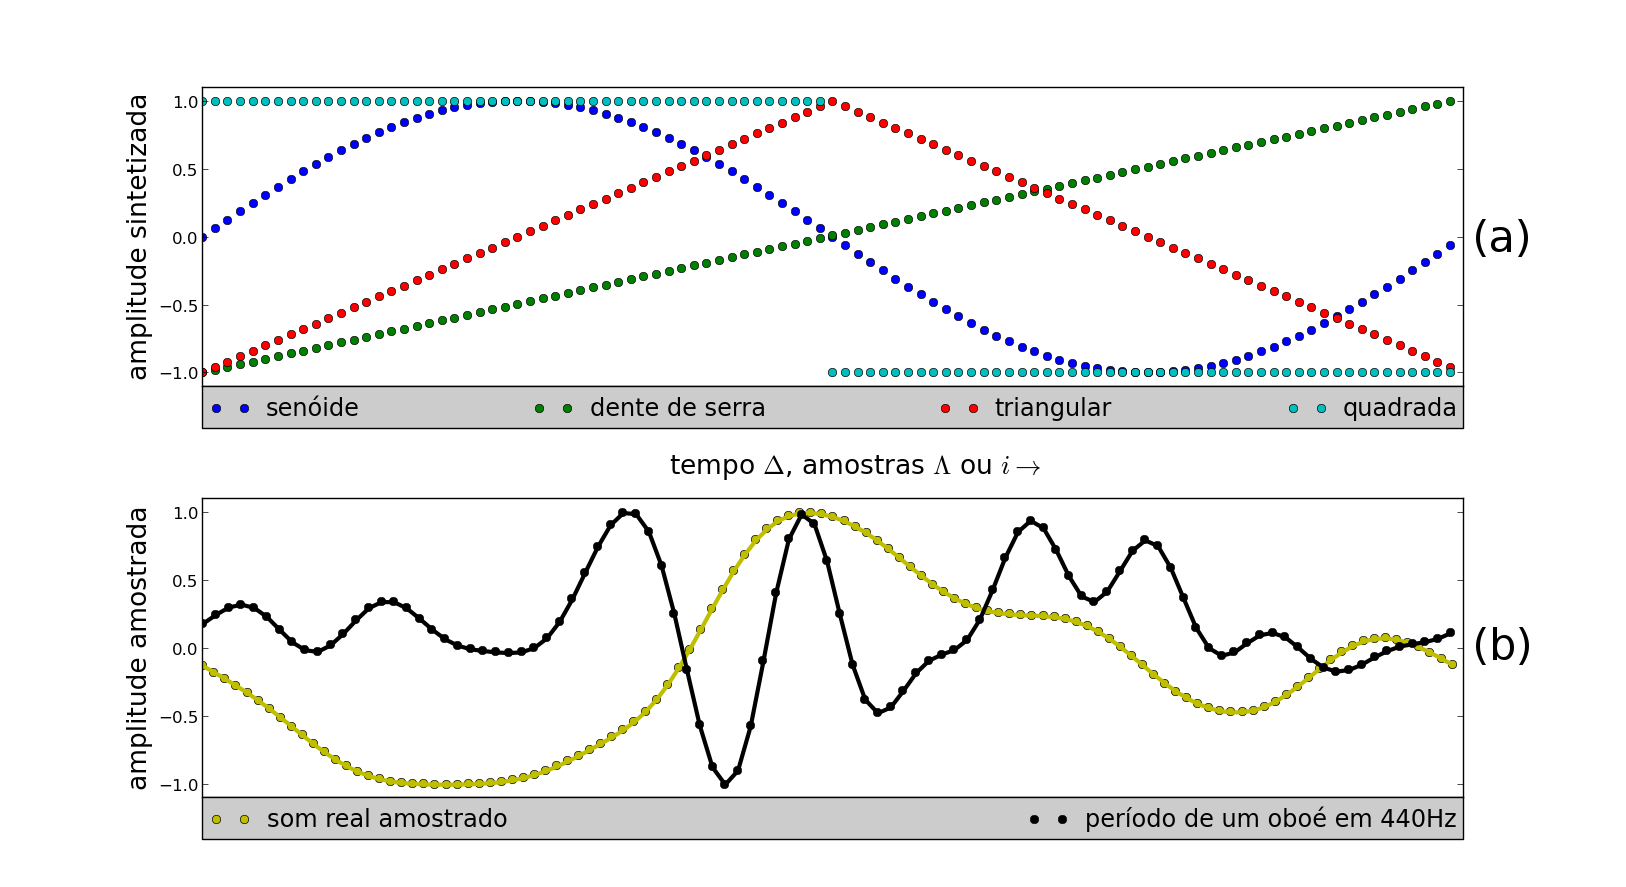
\includegraphics[width=\textwidth]{figuras/formasDeOnda6}
    \caption{Formas de onda musicais básicas. As formas de onda sintéticas estão em (a) e as formas de onda reais estão em (b).}
        \label{fig:formasDeOnda}
\end{figure}



A figura ~\ref{fig:formasDeOnda} apresenta
as formas de onda descritas nas equações ~\ref{senoide}, ~\ref{denteDeSerra}, ~\ref{triangular} e ~\ref{quadrada} para $\lambda_f=100$ (período
de $100$ amostras).
Se $t_a=44,1 kHz$, como no padrão PCM de \emph{Compact Disks}, a onda possui frequência fundamental $f=\frac{f_a}{\lambda_f}=\frac{44100}{100} = 441 \; Herz $. Um lá\footnote{Um lá 4, logo acima do dó central, no segundo espaço do pentagrama na clave de sol comum.}, independente da forma de onda.

O espectro de cada forma de onda básica está na figura ~\ref{fig:espectroDeOndas}. As componentes isoladas e exatamente harmônicas dos espectros correspondem a um período rigorosamente fixo. A senoide consiste de um nódulo único no espectro, frequência pura. A dente de serra é a única com a série harmônica completa (pares e ímpares). Já as ondas triangular e quadrada possuem as mesmas componentes espectrais, mas com decaimentos de $-12dB/oitava$ e $-6dB/oitava$ respectivamente.

\begin{figure}[h!]
    \centering
        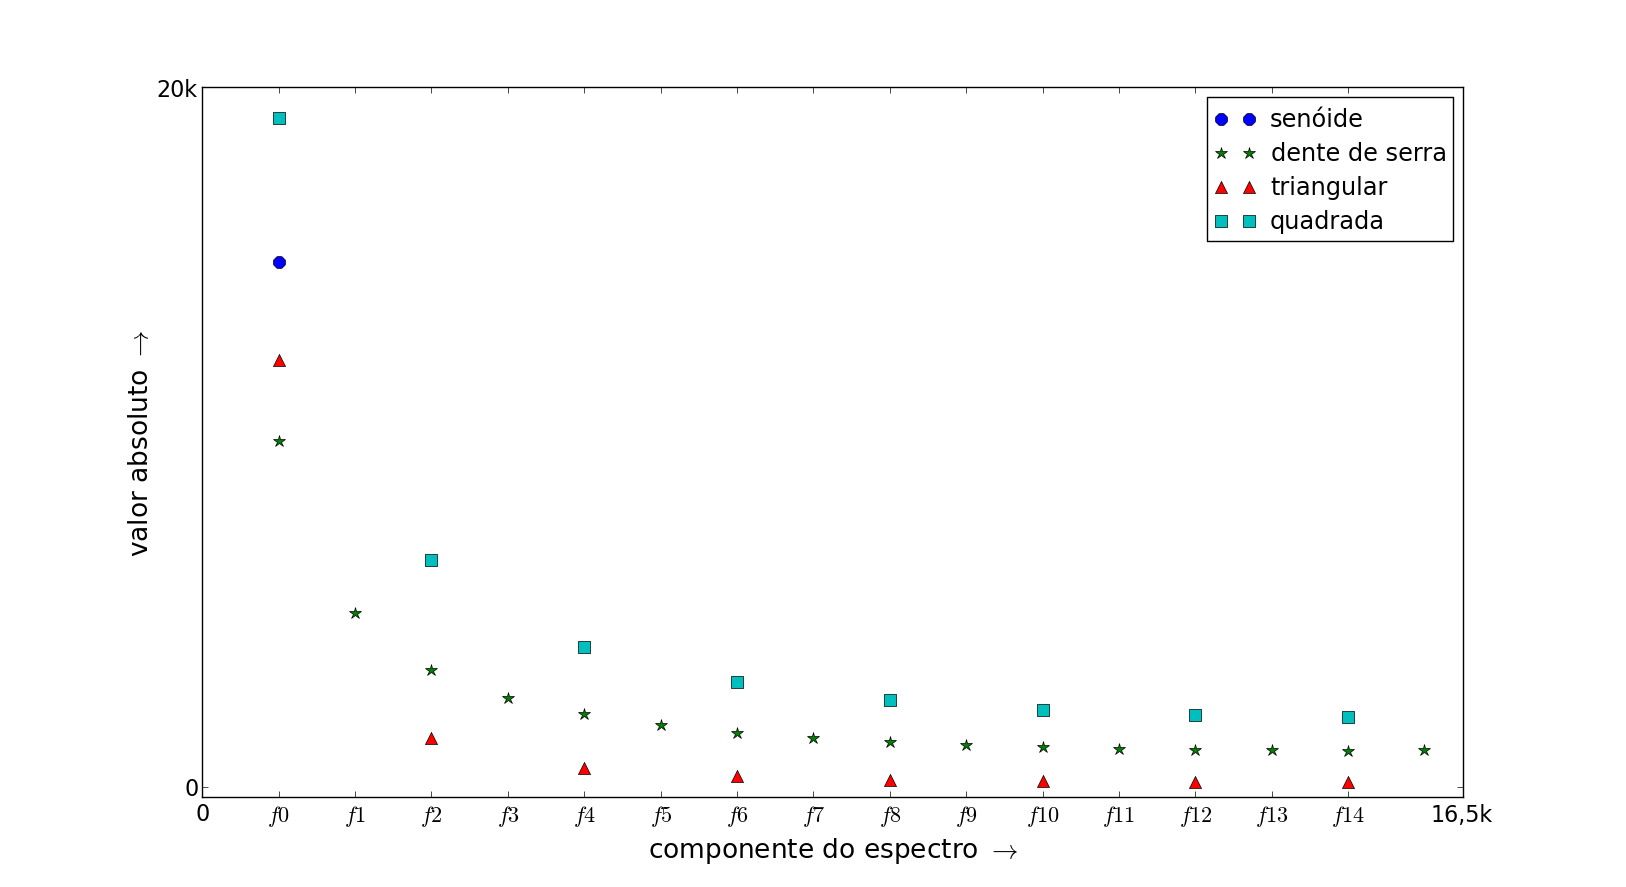
\includegraphics[width=\textwidth]{figuras/espectroDeOndas6}
    \caption{Espectros das ondas sonoras musicais artificiais básicas. As senoide tem o especro puntual, a triangular apresenta somente os harmônicos ímpares, caindo a 6dB por oitava; a onda quadrada tem somente os harmônicos ímpares, caindo a 12dB por oitava; a onda dente de serra apresenta todos os harmônicos, caindo a 6dB por oitava.}
        \label{fig:espectroDeOndas}
\end{figure}


O espectro harmônico é formado pelas frequências múltiplas da frequência fundamental $f_n=(n+1).f_0$.
Como a percepção humana de altura segue uma progressão geométrica de frequências, o espectro possui notas diferentes da frequência fundamental. Além disso, o número de harmônicos será limitado pela frequência máxima $f_a/2$ (pelo Teorema de Nyquist). 

Musicalmente crucial aqui é internalizar que a presença de
energia
em uma componente de frequência $f_n$ significa
 uma oscilação na constituição do som, puramente harmônica e naquela frequência $f_n$. Esta energia concentrada especificamente na frequência $f_n$ é separada
 pelo ouvido para adentrar em um nível cognitivo de processamento\footnote{Esta separação em frequência é realizada por diversas espécies através de mecanismos similares à cóclea humana.\cite{Roederer}}.
  As componentes senoidais são geralmente as principais responsáveis pela qualidade chamada timbre. Caso não se apresentem em proporções harmônicas (relações de pequenos números), o som é percebido como ruidoso ou dissonante e não com uma sonoridade de frequência fundamental estabelecida de forma unívoca. Além disso, a noção de altura absoluta em um complexo sonoro é baseada na semelhança do espectro com a série harmônica.\cite{Roederer}

No caso de uma forma de onda fixa e de tamanho fixo, o espectro é sempre harmônico e estático. Cada forma de onda é composta de proporções específicas das componentes harmônicas e 
quanto maior a curvatura do trecho na forma de onda, maior a contribuição do trecho para a
concentração de energia nos harmônicos agudos. Pode-se constatar isso em sons reais. A onda rotulada como ``som real amostrado'' na figura ~\ref{fig:formasDeOnda} é um período de $\lambda_f=114$ amostras extraído de um som real relativamente comportado. A onda de oboé foi amostrada de um lá 4 também em $44,1kHz$.
O período escolhido para a amostragem é relativamente curto, com 98 amostras corresponde a 
uma frequência de $\frac{44100}{98}=450 Hz$. Pode-se perceber, através das curvaturas, o espectro rico em 
frequências agudas do oboé e o espectro mais grave do som real.

A sequência 
$ R_i=\{ r_i \}_0^{\lambda_f-1}$ de amostras do som real da figura ~\ref{fig:formasDeOnda}
 pode ser tomada como base para um som $T_i^f$ da seguinte forma: 

\begin{equation}\label{sampleandoFormaDeOnda}
     T^f_i=\{ t_i^f \}=\Bigl\{ r_{(i\,\%\lambda_{f})} \Bigr\}
\end{equation}

O som resultante possui o espectro momentâneo do som original. Por ser repetido de forma idêntica,
seu espectro é perfeitamente harmônico, sem os ruídos e variações típicas do fenômeno natural. Isso pode ser 
visto na figura~\ref{fig:espectroOboe}, que mostra os espectros da nota original do oboé e de uma nota 
artificial de mesma duração e cujas amostras consistem no mesmo período da figura~\ref{fig:formasDeOnda}. O espectro natural possui variações nas frequências dos harmônicos, nas suas intensidades e uma quantidade de ruído. Já a nota cujo período foi amostrado possui espectro perfeitamente harmônico.



\begin{figure}[h!]
    \centering
        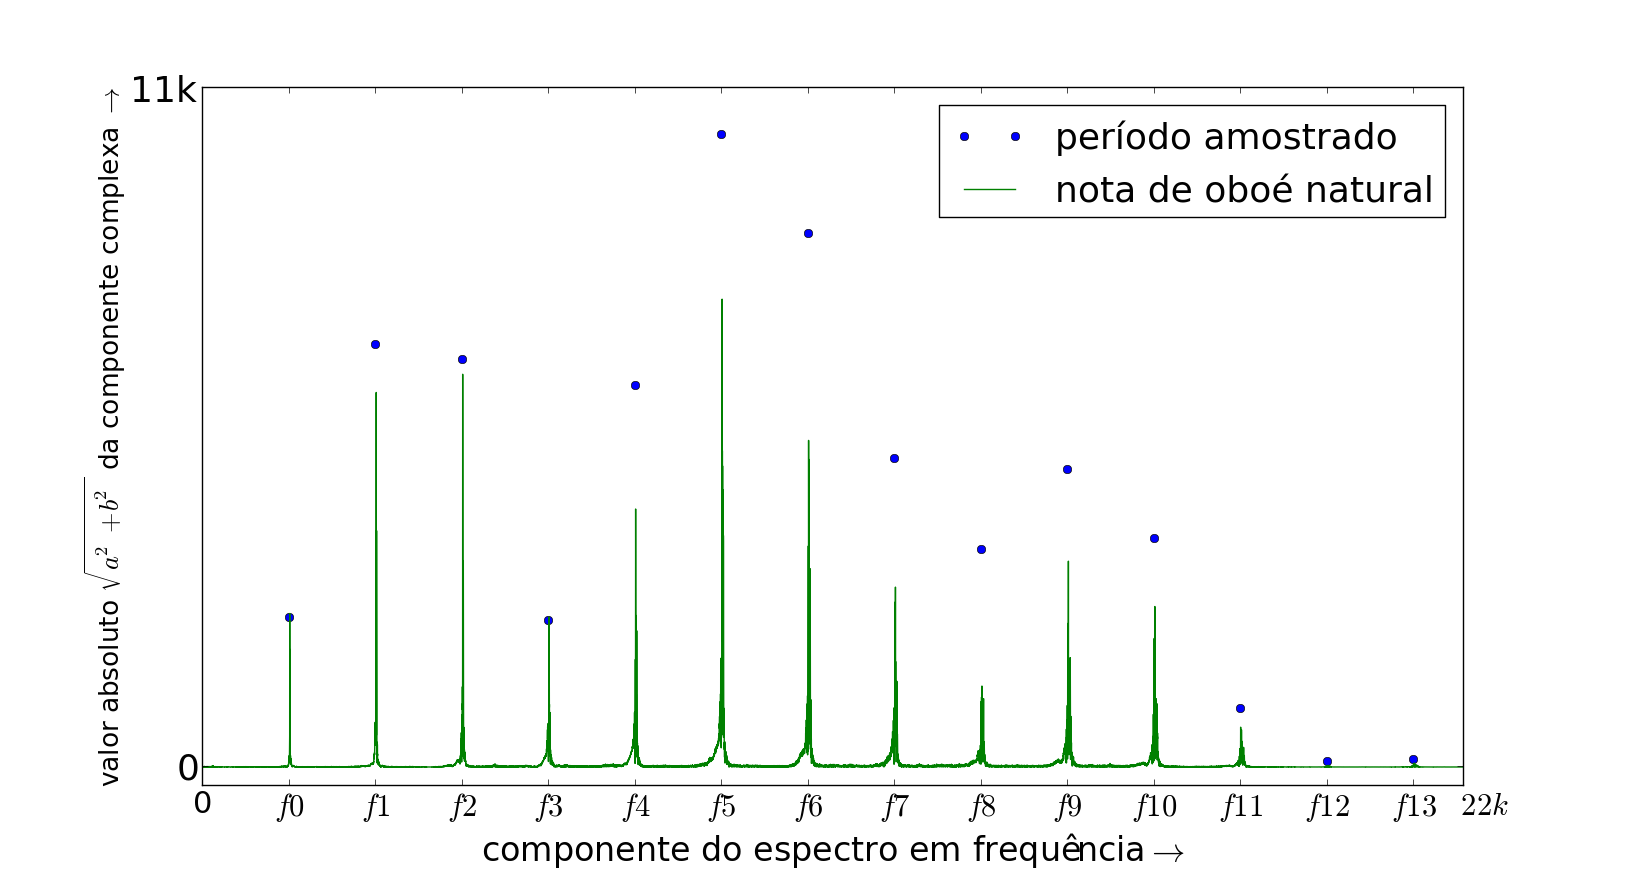
\includegraphics[width=\textwidth]{figuras/espectroOboeAmostradoNatural3}
    \caption{Espectros das ondas sonoras de uma nota de oboé natural e de período amostrado. O som natural possui flutuações nos harmônicos e ruídos, já o som de período amostrado possui espectro perfeitamente harmônico.}
        \label{fig:espectroOboe}
\end{figure}





\subsection{O espectro no som amostrado}
A presença e comportamento destas componentes senoidais 
no som discretizado possui particularidades. Considere um sinal $T_i$ e sua decomposição de Fourier $\mathcal{F}\langle T_i\rangle=C_i=\{c_i\}_0^{\Lambda-1}$. A recomposição é a soma das componentes frequenciais em amostras temporais\footnote{Lembrando que o fator $\frac{1}{\Lambda}$ pode ser distribuído dentre a transformada e a reconstrução como preferir.}:

 
\begin{equation}\label{recomposicaoFourier}
t_i = \frac{1}{\Lambda}\sum_{k=0}^{\Lambda-1}c_ke^{j \frac{2\pi k}{\Lambda} i } = \frac{1}{\Lambda}\sum_{k=0}^{\Lambda-1}(a_k+ j . b_k)\left[cos(w_k i) +j . sen(w_k i)\right]
\end{equation}

Onde $c_k = a_k + j . b_k$ dita a amplitude e fase de cada frequência: $w_k=\frac{2\pi}{\Lambda}k$ em radianos ou $f_k=w_k\frac{f_a}{2\pi}=\frac{f_a}{\Lambda}k$ em Herz,com atenção para os respectivos limites em $\pi$ e em $\frac{f_a}{2}$ dados pelo Teorema de Nyquist. 

No caso específico de um sinal sonoro, as amostras $t_i$ são reais e dadas pela parte real da equação ~\ref{recomposicaoFourier}:

\begin{equation}\label{moduloEfase}
\begin{split}
t_i& = \frac{1}{\Lambda}\sum_{k=0}^{\Lambda-1}\left[a_k cos(w_k i) -b_k sen(w_k i)\right] \\
   & = \frac{1}{\Lambda}\sum_{k=0}^{\Lambda-1}\sqrt{a_k^2 + b_k^2} \; cos\left[w_k i - tg^{-1}\left(\frac{b_k}{a_k}\right)\right]
\end{split}
\end{equation}

A equação ~\ref{moduloEfase} mostra que o termo imaginário de $c_k$ acrescenta uma fase à senoide real, i.e. os termos imaginários $b_k$ da decomposição espectral por Fourier proporcionam a varredura de fase
 $\left[-\frac{\pi}{2},+\frac{\pi}{2}\right]$ dada pelo termo $tg^{-1}\left(\frac{b_k}{a_k}\right)$ que possui esta imagem. O sinal de $a_k$ especifica o lado direito ou esquerdo do circulo trigonométrico,  o que completa a varredura de fase: $\left[-\frac{\pi}{2},+\frac{\pi}{2}\right] \cup \left[\frac{\pi}{2},\frac{3\pi}{2}\right]\equiv [2\pi]$.


\begin{figure}[h!]
    \centering
        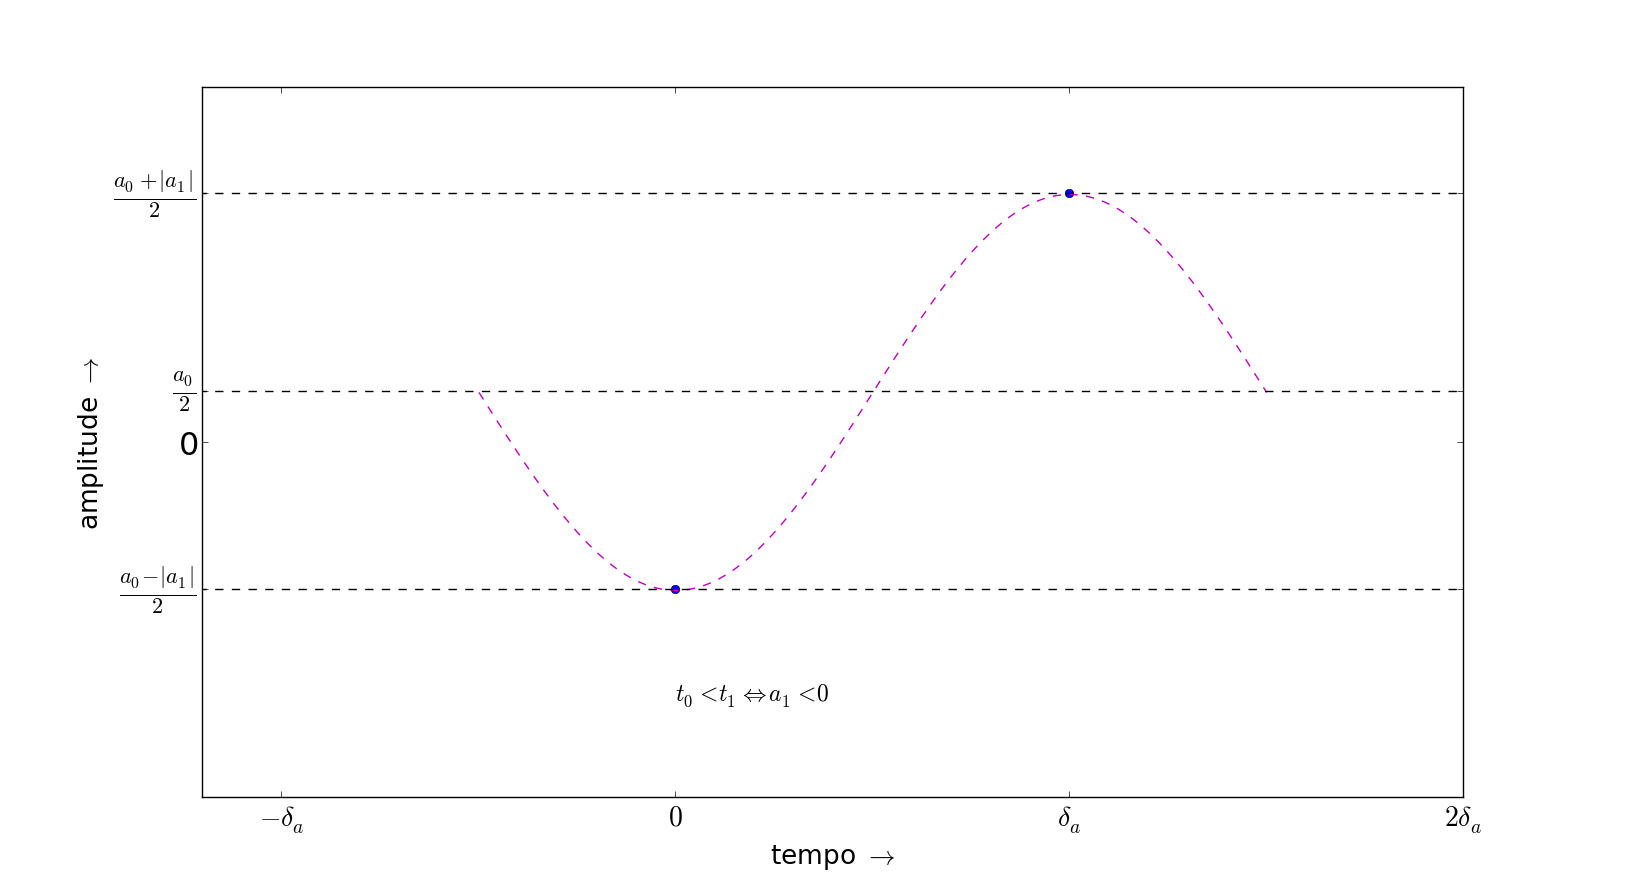
\includegraphics[width=\textwidth]{figuras/amostras2c__}
    \caption{Oscilação de 2 amostras (frequência máxima em qualquer $f_a$). O primeiro coeficiente reflete o deslocamento (\emph{offset} ou \emph{bias}) e o segundo coeficiente especifica a amplitude da oscilação.}
        \label{fig:amostras2}
\end{figure}

A figura ~\ref{fig:amostras2} exibe duas amostras e as componentes espectrais que contêm. A decomposição de Fourier possui neste caso um único par de coeficientes $\{c_k=a_k-j.b_k\}_0^{\Lambda-1=1}$ relativos às frequências $\{f_k\}_0^1=\left\{w_k\frac{f_a}{2\pi}\right\}_0^1=\left\{k\frac{f_a}{\Lambda=2}\right\}_0^1=\left\{0,\frac{f_a}{2}=f_{\text{máx}}\right\}$
com energias $e_k=\frac{(c_k)^2}{\Lambda=2}$. O papel das amplitudes $a_k$ é nítido com
 $\frac{a_0}{2}$ o deslocamento fixo\footnote{Chamado de \emph{bias} ou \emph{offset}.} e $\frac{a_1}{2}$ a amplitude da oscilação em si, dada pela relação $f_k=k \frac{f_a}{\Lambda=2}$.
Este caso é de especial importância pois o mínimo necessário para representar uma oscilação são 2 amostras e disso resulta a frequência de Nyquist $f_{\text{máx}}=\frac{f_a}{2}$. Esta é a frequência máxima presente em um som amostrado com $f_a$ amostras por segundo\footnote{Qualquer sinal amostrado possui esta característica, não somente o som digitalizado.}.

Todas as sequências fixas $T_i$ de apenas $3$ amostras também apresentam
somente $1$ frequência, pois sua primeira harmônica usaria $1.5$ amostras e ultrapassa o limite inferior de 2 amostras mínimas, i.e. a frequência da harmônica ultrapassaria a de Nyquist pois:  $\; \frac{2. f_a}{3} > \frac{f_a}{2} $. 
Os coeficiêntes $\{c_k\}_0^{\Lambda-1=2}$ apresentam-se em 
3 componentes frequenciais. Uma delas é relativa à frequência zero ($c_0$), as outras duas ($c_1$ e $c_2$) contribuem de forma igual na reconstrução da senoide com $f=f_a/3$.

\begin{figure}[h!]
    \centering
        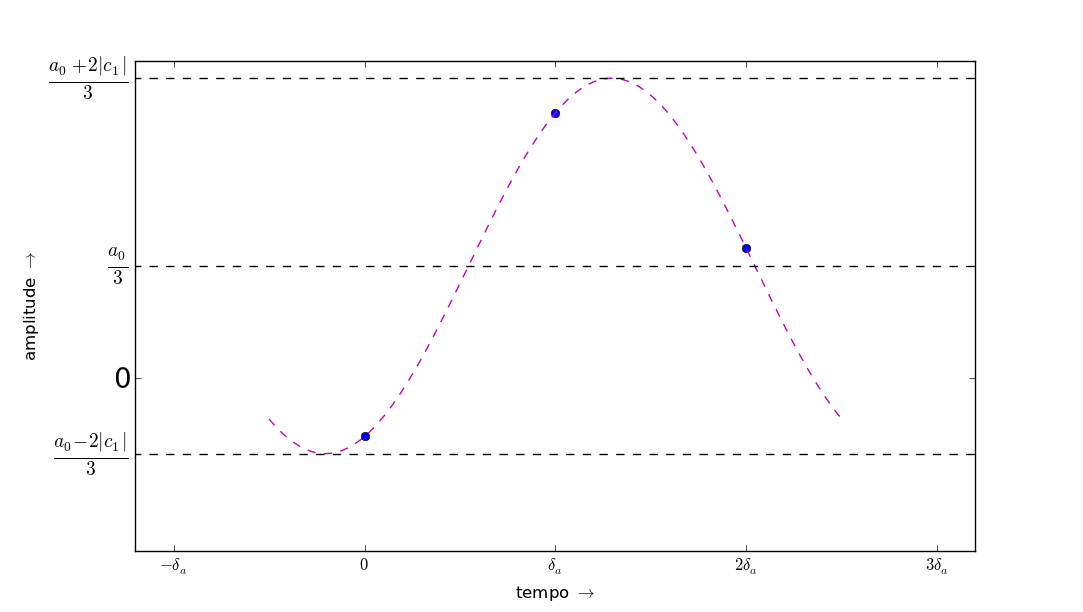
\includegraphics[width=\textwidth]{figuras/amostras3b}
    \caption{3 amostras fixas apresentam uma só frequência não nula. $c_1=c_2^*$ e $w_1 \equiv w_2$.}
        \label{fig:amostras3}
\end{figure}



$\Lambda$ amostras reais $t_i$ resultam em $\Lambda$ coeficientes complexos $c_k=a_k+j.b_k$. Os coeficientes $c_k$ se equivalem dois a dois correspondendo às mesmas frequências e com contribuições idênticas\footnote{Parte real igual e imaginária com sinal trocado: $a_{k1}=a_{k2}$ e $b_{k1}=-b_{k2}$. Como consequência os módulos são iguais e as fases possuem sinais opostos}. Lembrando que $f_k = k\frac{f_a}{\Lambda}, \; k \in \left\{0, ..., \left \lfloor \frac{\Lambda}{2} \right \rfloor \right\} $. Quando $k> \frac{\Lambda}{2} $,
a frequência $f_k$ é espelhada em $\frac{f_a}{2}$ da seguinte forma $f_k=\frac{f_a}{2} - (f_k-\frac{f_a}{2})=f_a-f_k=f_a - k\frac{f_a}{\Lambda}=(\Lambda-k)\frac{f_a}{\Lambda} \;\;\;\; \Rightarrow \;\;\;\; f_k\equiv f_{\Lambda-k} \; ,\;\; \forall \;\; k<\Lambda$. 

 
 O mesmo pode ser observado com 
 $w_k=f_k.\frac{2\pi}{f_a}$ e lembrando da periodicidade $2\pi$, que resulta em $w_k=-w_{\Lambda-k}$. Como o coseno é uma função par e a tangente inversa é impar, as componentes em $w_k$ e $w_{\Lambda-k}$ se somam na equação de reconstrução das amostras reais disposta na equação~\ref{recomposicaoFourier}.

  Ou seja, em uma decomposição de $\Lambda$ amostras, as $\Lambda$ componentes frequenciais $\{c_i\}_0^{\Lambda-1}$ resultantes
   são equivalentes em pares.
   Exceção para $f_0$ e, no caso de $\Lambda$ ser par, de $f_{\Lambda/2}=f_{\text{máx}}=\frac{f_a}{2}$ , ambas as componentes são isoladas, i.e. não existe outra componente na frequência $f_0$ ou $f_{\Lambda/2}$ (se $\Lambda$ par) além dela mesma. 
Pois $f_{\Lambda/2}=f_{(\Lambda-\Lambda/2) = \Lambda/2}$ e $f_0=f_{(\Lambda-0)=\Lambda}=f_0$.
Além disso, estas duas frequências (a frequência zero e a frequência máxima) não são representadas com variação de fase e, portanto, são estritamente reais. Assim, pode-se
   concluir que o número $\tau$ de pares de coeficientes equivalentes é:

\begin{equation}\label{coefsPareados}
\tau = \frac{\Lambda - \Lambda \% 2}{2} +\Lambda \% 2 -1
\end{equation}

e ficam evidentes as equivalências ~\ref{equivalenciasFreqs}, ~\ref{equivalenciasModulos} e ~\ref{equivalenciasFases}:

\begin{equation}\label{equivalenciasFreqs}
f_{k}\equiv f_{\Lambda-k}\;, \;\; w_{k}\equiv-w_{\Lambda-k}\;\;\;, \quad \;\; \forall \quad 1 \leq k \leq \tau  
\end{equation}

\begin{figure}[h!]
    \centering
        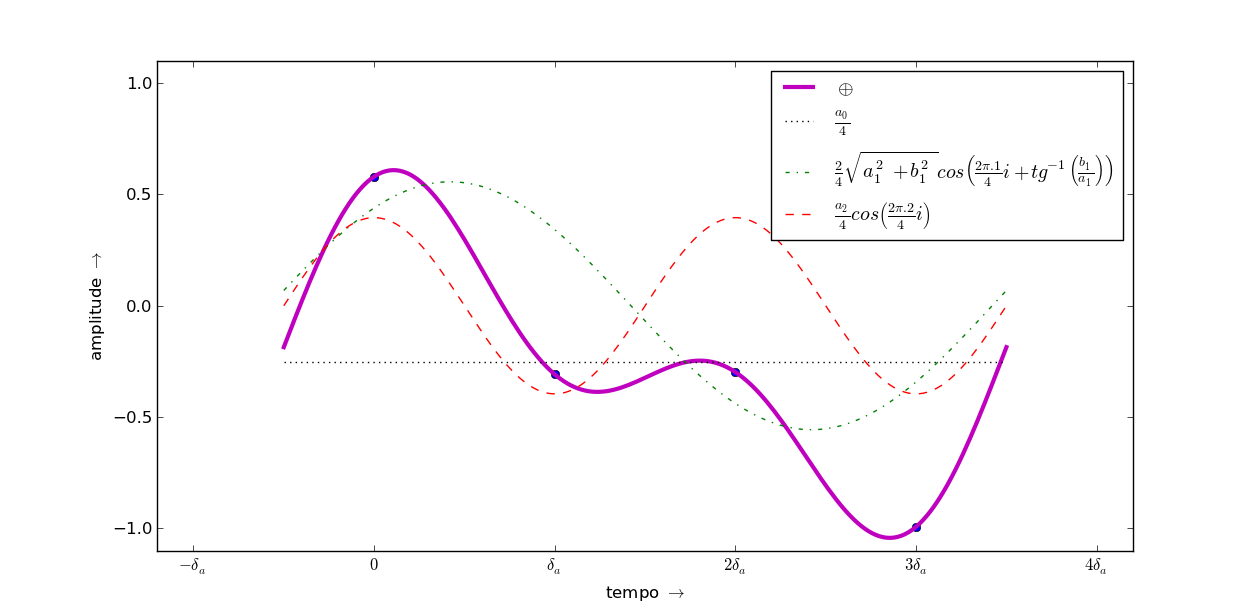
\includegraphics[width=\textwidth]{figuras/amostras4__}
    \caption{Componentes frequenciais em 4 amostras.}
        \label{fig:amostras4}
\end{figure}


Como $a_k = a_{\Lambda -k}\;\;$ e $\;\;b_k = - b_{\Lambda -k}$:

\begin{equation}\label{equivalenciasModulos}
\sqrt{a_k^2 + b_k^2} = \sqrt{a_{\Lambda - k}^2 + b_{\Lambda -k}^2} \;\;, \quad \;\; \forall \quad 1 \leq k \leq \tau  \\
\end{equation}

\begin{equation}\label{equivalenciasFases}
tg^{-1}\left(\frac{b_k}{a_k}\right)=-tg^{-1}\left(\frac{b_{\Lambda -k}}{a_{\Lambda - k}}\right)\;\;,\quad \;\; \forall \quad 1 \leq k \leq \tau
\end{equation}



Com $k \in \mathbb{N}$.

 A observação da equação de reconstrução para o sinal real ~\ref{moduloEfase} em conjunto com as equivalências dos módulos e fases ~\ref{equivalenciasModulos} e ~\ref{equivalenciasFases}, o número de coeficientes pareados \ref{coefsPareados} e equivalência de pares de frequências \ref{equivalenciasFreqs}
expõe o caso geral da combinação das componentes em cada amostra $t_i$:

\begin{equation}\label{eq:reconsCompleta}
t_i = \frac{a_0}{\Lambda} + \frac{2}{\Lambda}\sum_{k=1}^{\tau}\sqrt{a_k^2 + b_k^2} \; cos\left[w_k i - tg^{-1}\left(\frac{b_k}{a_k}\right)\right]+ \frac{ a_{\Lambda/2}}{\Lambda}.(1-\Lambda\% 2)
\end{equation}

\begin{figure}[h!]
    \centering
        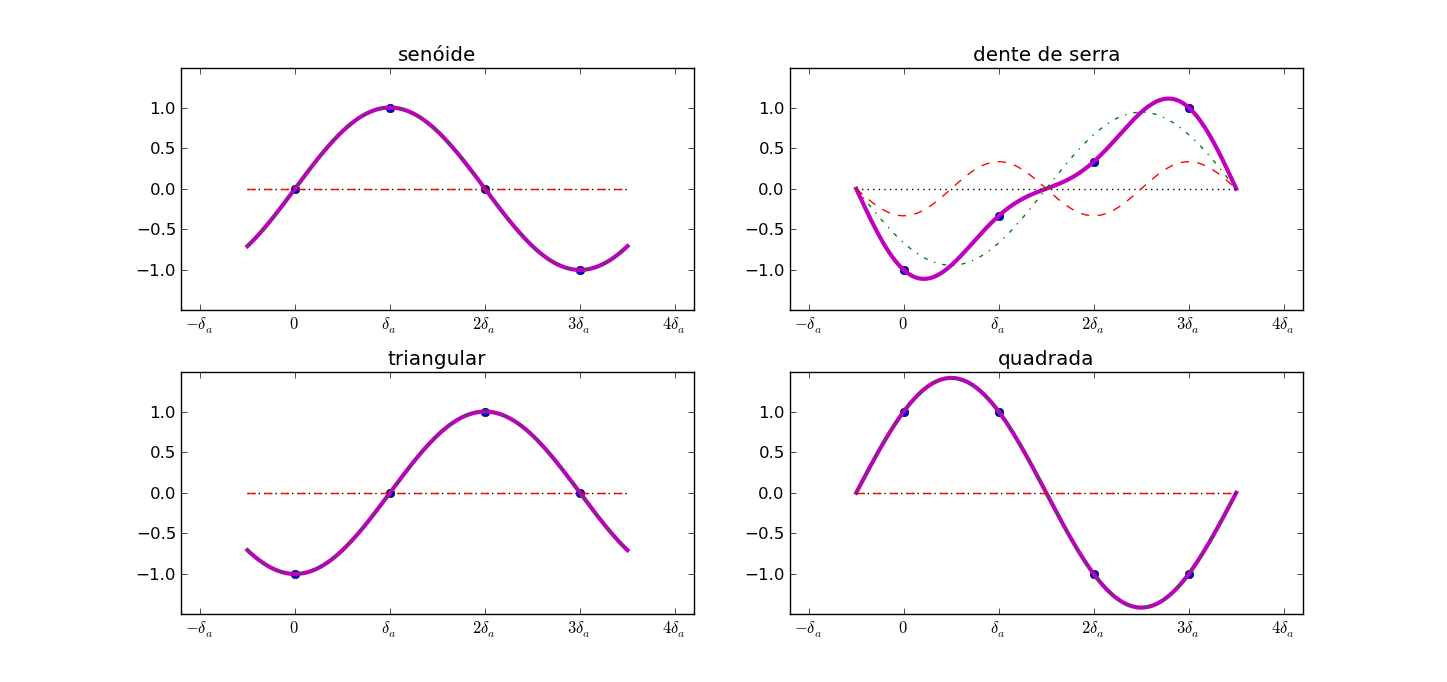
\includegraphics[width=\textwidth]{figuras/amostras4formas__}
    \caption{Formas de onda básicas em 4 amostras.}
        \label{fig:formas4}
\end{figure}


Assim, a exemplo da figura ~\ref{fig:amostras3}, a transformada de Fourier de 3 amostras possui 2 coeficientes frequenciais com quantidades iguais de energia na mesma frequência.

Com 4 amostras, pode-se representar 1 ou 2 frequências em proporções quaisquer. A figura ~\ref{fig:amostras4} mostra uma 
forma de onda de 4 amostras e suas duas componentes. 
As contribuições individuais se somam na forma de onda 
original, e uma breve inspeção revela que as curvaturas maiores são fruto da frequência mais aguda,
enquanto um deslocamento fixo da somatória das componentes advém
da componente na frequência zero.
\begin{figure}[h!]
    \centering
        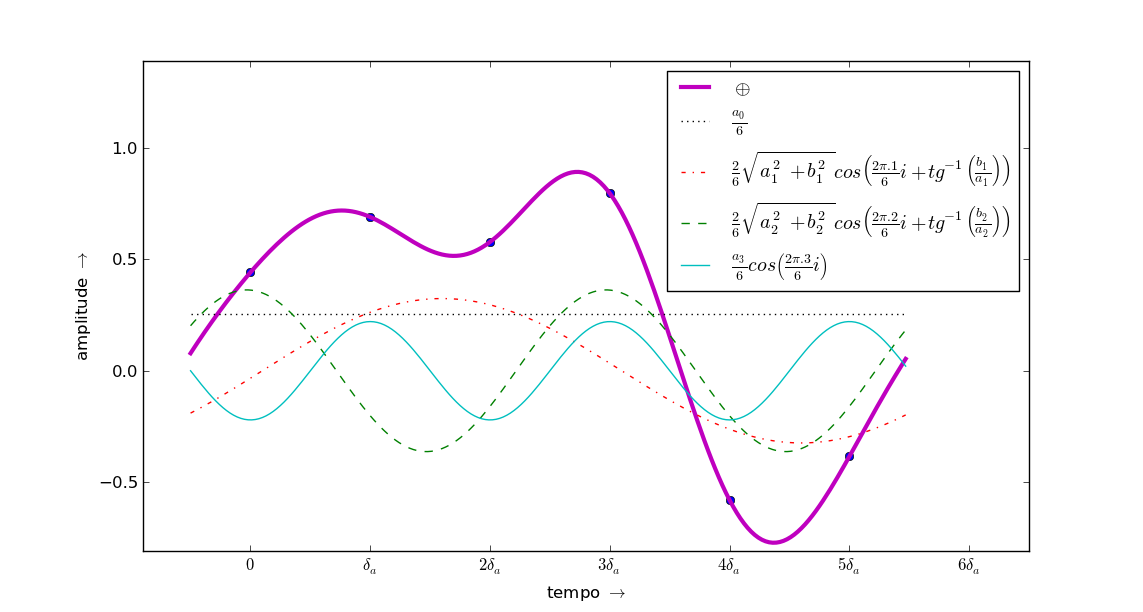
\includegraphics[width=\textwidth]{figuras/amostras6}
    \caption{Componentes frequenciais em 6 amostras: 3 senoides se somam ao \emph{bias}.}
        \label{fig:amostras6}
\end{figure}


A figura ~\ref{fig:formas4} explicita os harmônicos em 4 amostras nas formas de onda básicas das equações ~\ref{senoide}, ~\ref{denteDeSerra}, ~\ref{triangular} e ~\ref{quadrada}. Todas consistem em apenas 1 senoide, com exceção da dente de serra que possui os harmônicos pares.


A figura ~\ref{fig:amostras6} mostra uma decomposição senoidal para o caso de 6 amostras e a figura ~\ref{fig:formas6} decompõe as formas de onda básicas.
 Neste caso todas as ondas se diferenciam no espectro: as quadrada e triangular possuem as mesmas componentes, mas em proporções diferentes, já a dente de serra possui uma componente a mais.

\begin{figure}[h!]
    \centering
        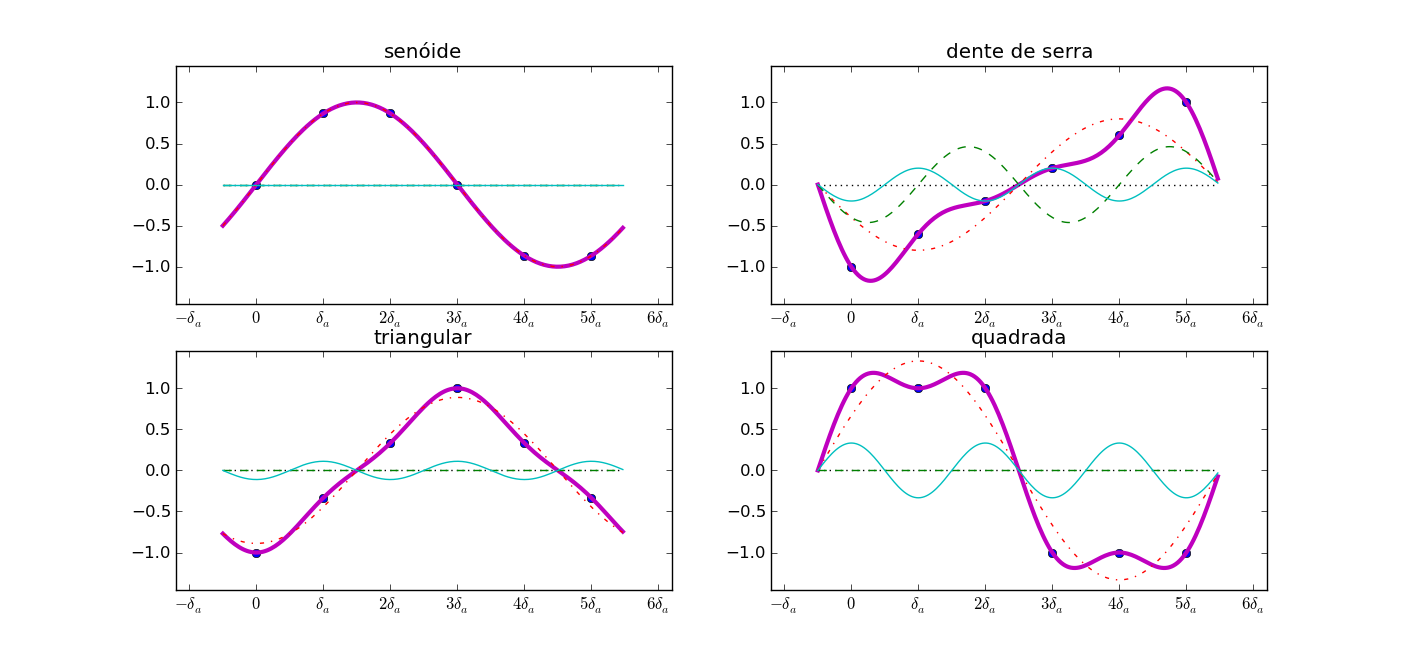
\includegraphics[width=\textwidth]{figuras/amostras6formas___}
    \caption{Formas de onda básicas em 6 amostras: as ondas triangular e quadrada possuem os harmônicos ímpares, mas em proporções e fases diferentes; a dente de serra possui também o harmônico par.}
        \label{fig:formas6}
\end{figure}



\subsection{A nota básica}\label{notaBasica}

Seja $f$ tal que $f$ divida $f_a$\footnote{Como apontado anteriormente, esta limitação facilita a exposição sem perda de generalidade.
A limitação será superada no início da próxima seção.}.
Uma sequência $T_i$ de amostras sonoras separadas por $\delta_a=1/f_a$ descreve uma nota musical de frequência $f$ Herz e duração $\Delta$ segundos se, e somente se, possuir a periodicidade $\lambda_f=f_a/f$
 e tamanho $\Lambda=\lfloor f_a . \Delta \rfloor $:

\begin{equation}\label{eq:notaBasica}
T_i^{f,\; \Delta}=\{t_{i \, \% \lambda_f} \}_0^{\Lambda-1}= \left \{t^f_{i \; \% \left( \frac{f_a}{f} \right) } \right \}_0^{\Lambda-1}
\end{equation}

A nota por si só não especifica um timbre. Mesmo assim, faz-se necessária a escolha de uma forma de onda para que as amostras $t_i$ tenham um valor estabelecido individualmente. Um único período dentre as ondas básicas pode ser utilizado para a especificação da nota da seguinte forma:

$\lambda_f=\frac{f_a}{f}$ é o número de amostras do período. Seja $L_i^{f,\, \delta_f} $
a sequência que descreve um período da onda $L_i^f \in \{S_i^f,Q_i^f,T_i^f,D_i^f,R_i^f \}$ de duração 
$\delta_f=1/f$, dadas pelas equações ~\ref{senoide}, ~\ref{denteDeSerra}, ~\ref{triangular} e ~\ref{quadrada} e onde $R_i^f$ é
uma onda real amostrada:

\begin{equation}\label{periodoUnico}
L_i^{f , \delta_f } = \left\{ l_i^f \right\}_0^{\delta_f . f_a -1}=\left\{ l_i^f \right\}_0^{\lambda_f-1}
\end{equation}

Então a sequência $T_i$ consistirá em uma nota de duração $\Delta$ e frequência $f$ se:

\begin{equation}\label{eq:notaBasicaTimbre}
T_i^{f,\; \Delta}=\left\{t_i^f\right\}_0^{\lfloor f_a . \Delta \rfloor -1}=\left \{ l^f_{i\,\%\left(\frac{f_a}{f}\right)} \right \}_0^{\Lambda-1}
\end{equation}

\subsection{Localização espacial}
Embora não seja uma das quatro qualidades básicas tradicionais de uma nota musical, esta possui sempre uma localização espacial. Além disso, a espacialização é atributo bastante valorizado
 por audiófilos e pela indústria fonográfica.\cite{floEsp}
Acredita-se que a percepção da localização espacial do som se dê em nosso sistema nervoso através destas
três informações: o atraso de chegada do som entre um ouvido e o outro, a diferença de intensidade do som direto em cada ouvido e a 
filtragem realizada pelo corpo, incluindo toráx, cabeça e orelhas.\cite{Roederer, hrtf, Heeger}


\begin{figure}[h!]
    \centering
        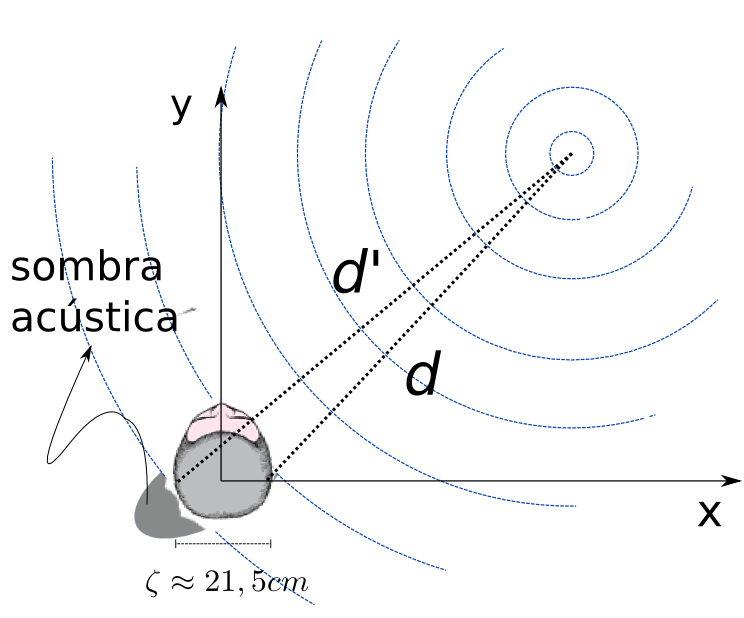
\includegraphics[width=.5\textwidth]{figuras/espacializacao___}
    \caption{Detecção de localização espacial de fonte sonora: esquema utilizado para cálculo da diferença de tempo interaural (DTI) e da diferença de intensidade interaural (DII).}
        \label{fig:spac}
\end{figure}



	Se consideradas somente as incidências diretas em cada ouvido, as equações são simples. Dada a separação $\zeta$ entre os ouvidos\footnote{Constata-se que $\zeta \approx 21,5cm$ para um humano adulto.},
um objeto localizado em $(x,y)$ conforme a figura~\ref{fig:spac}
está distante de cada ouvido:

\begin{equation}\label{eq:distOuvidos}
\begin{split}
d & =\sqrt{\left (x-\frac{\zeta}{2} \right )^2+y^2} \\
d' & =\sqrt{\left (x+\frac{\zeta}{2} \right )^2 + y^2}
\end{split}
\end{equation}


e cálculos imediatos resultam na Diferença de Tempo Interaural:

\begin{equation}\label{eq:dti}
DTI=\frac{d'-d}{v_{som\;no\;ar}\approx 343.2 }\quad \text{segundos}
\end{equation}

e na Diferença de Intensidade Interaural:
\begin{equation}\label{eq:dii}
DII=20\log_{10}\left (\frac{d}{d'}\right) \quad decibels
\end{equation}

Convertendo para amplitude, obtem-se $DII_a=\frac{d}{d'}$. A $DII_a$ pode
ser utilizada como constante multiplicativa do canal direito de um sinal sonoro estéreo: $\{t_i'\}_0^{\Lambda -1}=\{DII_a . t_i\}_0^{\Lambda -1}$. Pode-se utilizar a DII junto à DTI como adiantamento no tempo do canal direito com relação ao esquerdo, vínculo crucial para a localização em sons graves e em sonoridades percussivas.\cite{Heeger}  
Considerando $\Lambda_{DTI}=\lfloor DTI . f_a \rfloor$:

\begin{equation}\label{eq:locImpl}
\begin{split}
\Lambda_{DTI} & = \left \lfloor \frac{d'-d}{343,2}  f_a \right \rfloor \\
DII_a & = \frac{d}{d'} \\
\left\{t_{(i+\Lambda_{DTI})}'\right\}_{\Lambda_{DTI}}^{\Lambda+\Lambda_{DTI}-1} & =\left\{DII_a . t_i\right\}_0^{\Lambda-1} \\
\left\{t_i'\right\}_0^{\Lambda_{DTI}-1} & = 0
\end{split}
\end{equation}

Com $t_i$ o canal direito e $t_i'$ o canal esquerdo. Caso $\Lambda_{DTI} < 0 $, basta trocar $t_i$ por $t_i'$  e utilizar $\Lambda_{DTI}'= | \Lambda_{DTI} | $.

Embora consideravelmente simples até aqui, a localização espacial depende drasticamente de outras pistas. Pela
DTI e DII especifica-se somente o ângulo horizontal (azimutal) $\theta$ dado por:

\begin{equation}\label{eq:angulo}
\theta=\tan^{-1}\left ( \frac{y}{ x }  \right )
\end{equation}

com $x,y$ tais como representados na figura~\ref{fig:spac}. Mesmo assim, há dificuldades quando $\theta$ incide sobre o chamado "cone de confusão" em que um mesmo par de especificações DTI, DII resultam de vários dos pontos 
do cone. Nestes pontos, a inferência do ângulo azimutal depende especialmente da filtragem atenuante nos agudos, pois a cabeça interfere um tanto mais nas ondas mecânicas agudas do que nas graves.\cite{Heeger,hrtf} 

A figura~\ref{fig:spac} mostra também esta sombra acústica do crânio, importante para a percepção do ângulo azimutal da fonte no cone de confusão. O cone em si não foi disposto na figura pois não é exatamente um cone e suas dimensões precisas não foram encontradas na literatura visitada, mas pode ser entendido como um cone com o ápice no meio da cabeca e saindo por cada uma das orelhas.\cite{hrtf}

Já a localização completa, incluindo distância e elevação da fonte sonora, é dada pela função de transferência de cabeça (HRTF - do inglês \emph{Head Related Transfer Function}).\cite{hrtf} Exitem bases abertas e conhecidas de HRTF como a CIPIC e pode-se aplicar estas funções de transferência em um som por convolução (veja equação~\ref{eq:conv}).\cite{CIPIC} O corpo do indivíduo altera bastante as filtragens realizadas e existem técnicas para gerar HRTFs que sejam - como proposta - utilizáveis de forma universal.\cite{lazaSPA} 



\subsection{Usos musicais}\label{subsec:basMus}


A partir da nota básica, cabe realizar estruturas musicais com
sequências destas partículas. A soma dos elementos de mesmo índice de $N$ sequências $T_{k,i}=\{t_{k,i}\}_{k=0}^{N-1}$ de mesmo tamanho $\Lambda$ resulta em seus conteúdos espectrais sobrepostos em um processo de mixagem sonora:

\begin{equation}\label{eq:mixagem}
\{t_i\}_0^{\Lambda-1}=\left \{ \sum_{k=0}^{N-1}t_{k,i} \right \}_0^{\Lambda-1}
\end{equation}

\begin{figure}[h!]
    {\centering
        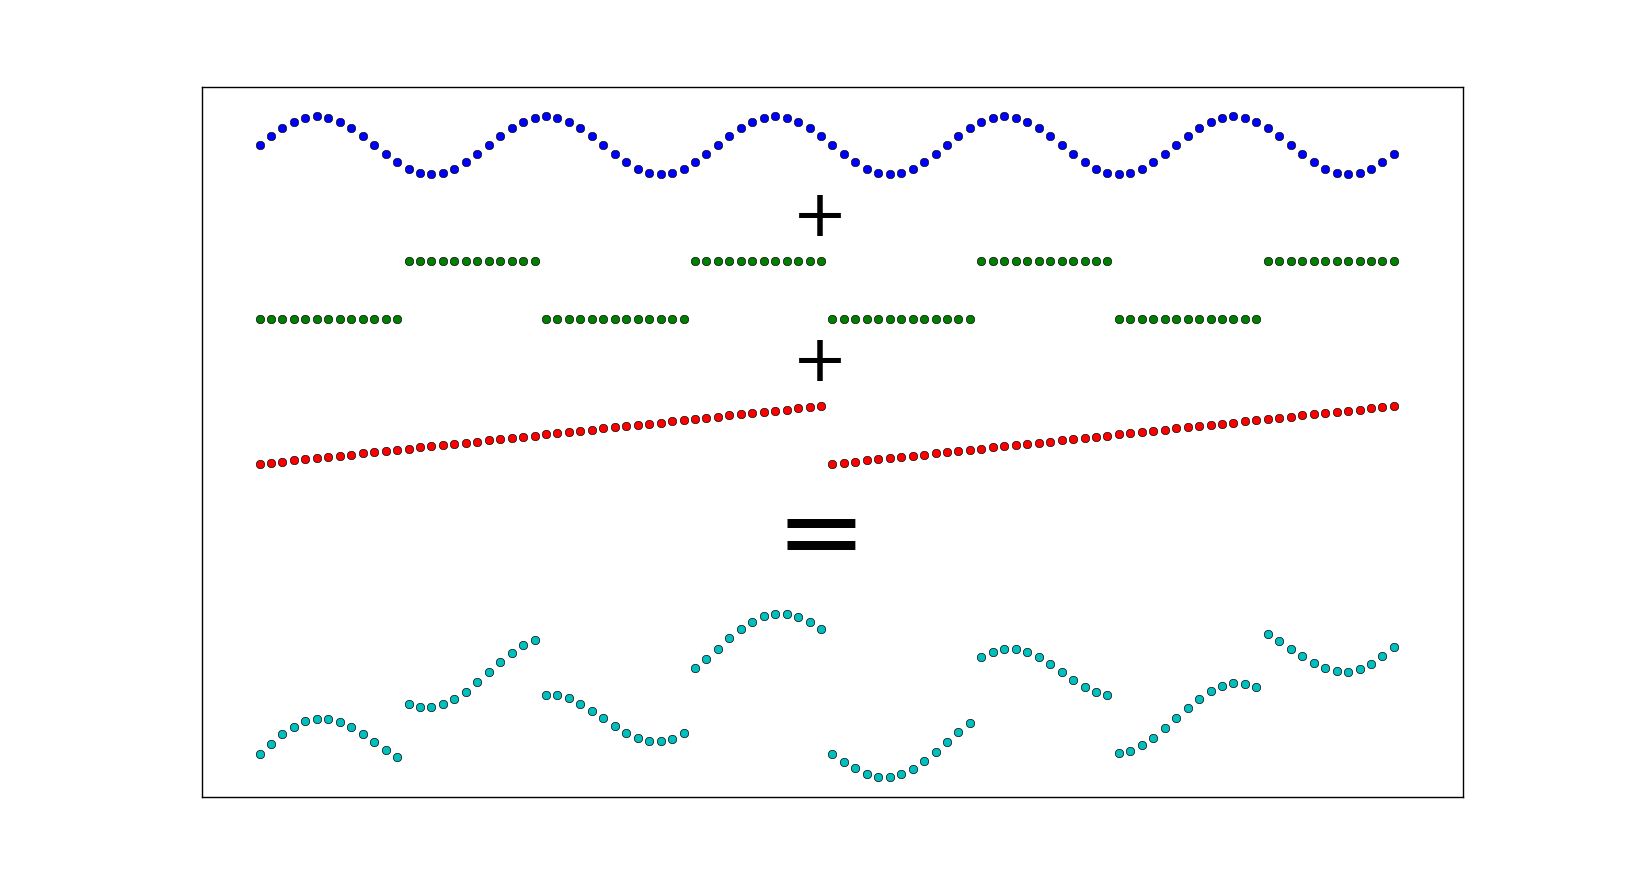
\includegraphics[width=\textwidth]{figuras/mixagem}}
    \caption{Mixagem de três sequências sonoras. As amplitudes são sobrepostas diretamente.}

        \label{fig:mixagem}
\end{figure}


A figura~\ref{fig:mixagem} ilustra este processo de superposição de ondas sonoras discretizadas. A figura dispõe 100 amostras, de onde pode-se concluir que, se $f_a=44.1kHz$, as frequências da dente de serra, da onda quadrada e da senoide são,
respectivamente, $\frac{f_a}{100/2}=882Hz$, $\frac{f_a}{100/4}=1764Hz$ e $\frac{f_a}{100/5}=2205Hz$. A duração do trecho é bastante curto $\frac{f_a=44.1kHz}{100} \approx 2 \text{ milisegundos}$. Basta completar com zeros para somar sequências de tamanhos diferentes. 

As notas mixadas são em grande parte separadas pelo ouvido por leis físicas de ressonância e pelo sistema nervoso.\cite{Roederer} O resultado da mixagem de notas musicais é a harmonia musical, cujos intervalos entre as frequências e os acordes de notas simultâneas regem aspectos subjetivos e abstratos da música e sua apreciação.\cite{Harmonia} 

As sequências podem também ser concatenadas no tempo. Caso as sequências $\{t_{k,i}\}_0^{\Lambda_k-1}$ de tamanhos $\Lambda_k$  representem $k$ notas musicais, sua concatenação em uma única sequência $T_i$ é em uma sequência musical simples ou melodia:

\begin{equation}\label{eq:concatenacao}
\{t_i\}_0^{\sum\Delta_k-1}=\{t_{l,i}\}_0^{\sum\Delta_k-1}, \;\; l\text{ menor inteiro } : \quad \Lambda_l > i -\sum_{j=0}^{l-1}\Lambda_j
\end{equation}

Este mecanismo é demonstrado de forma ilustrativa na figura~\ref{fig:concatenacao} com as mesmas sequências da figura ~\ref{fig:mixagem}.
 As sequências são curtas para as taxas de amostragem usuais, mas pode-se observar a concatenação de sequências sonoras. Além disso, cada nota tem a duração maior que $100ms$ se $f_a<1kHz$.

\begin{figure}[h!]
{    \centering
        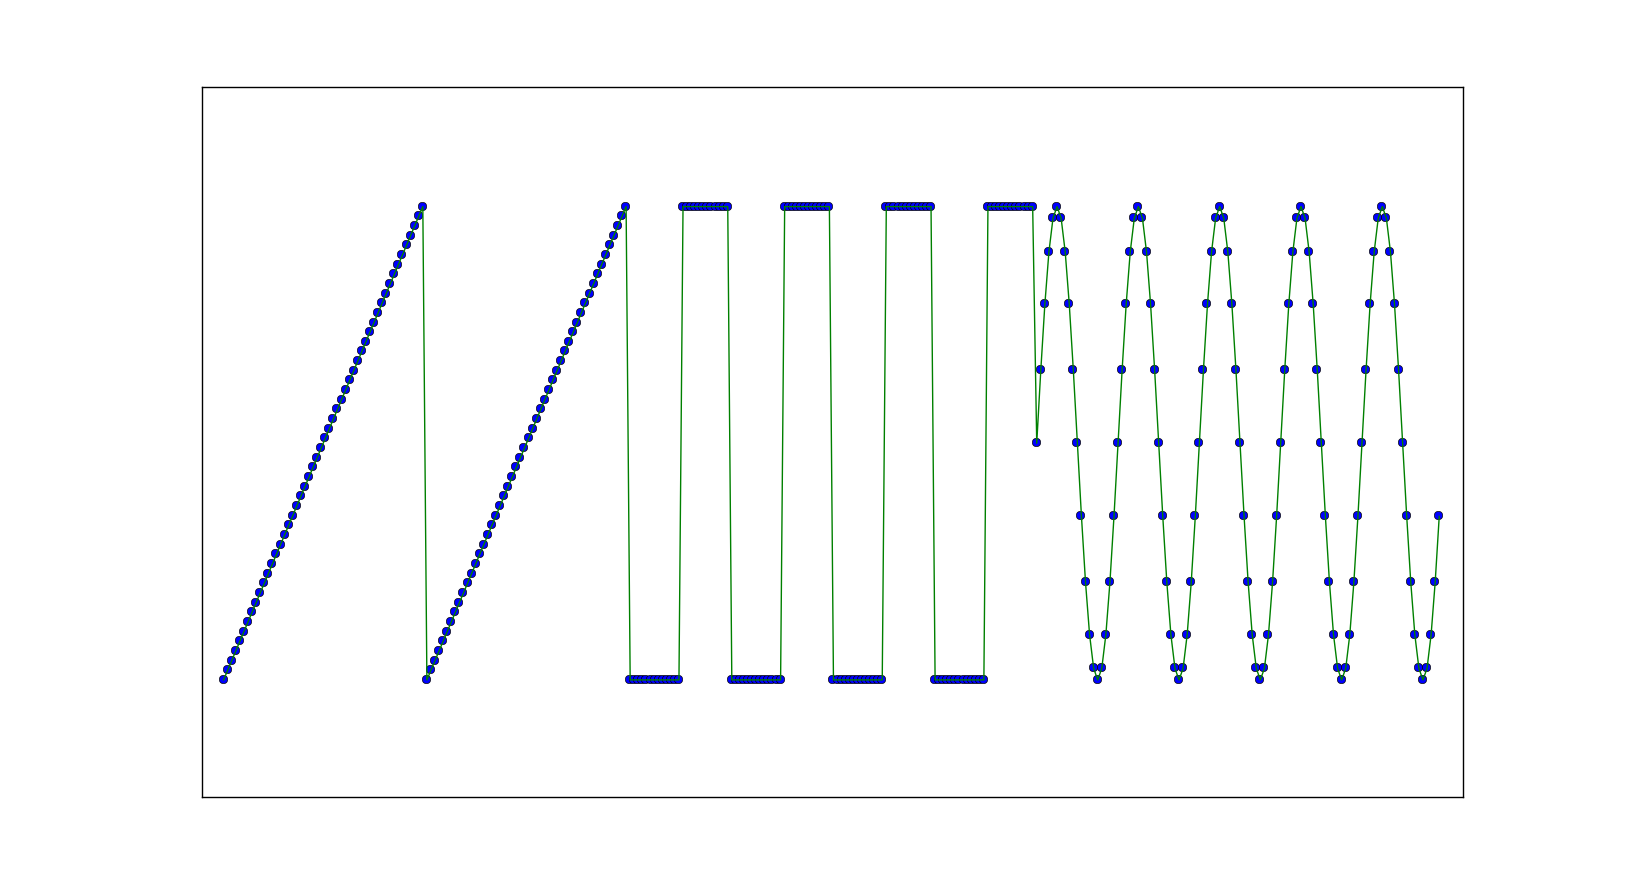
\includegraphics[width=\textwidth]{figuras/concatenacao}}
    \caption{Concatenação de três sequências sonoras através da justaposição temporal de suas amostras.}
        \label{fig:concatenacao}
\end{figure}

A montagem musical \emph{reduced-fi} explora de forma isolada este uso de justaposição temporal das notas, resultando em uma peça homofônica. O princípio vertical está demonstrado nos \emph{quadros sonoros}, sons estáticos com espectros peculiares. Ambas as peças estão em código Python nos Apêndices~\ref{ap:quadros} e~\ref{ap:reduced} e estão disponíveis como parte da \emph{toolbox} \massa.\cite{MASSA}

Está descrita a nota musical digital básica e a seção a seguinte desenvolve a evolução temporal de seus conteúdos, como nos glissandos e nas envoltórias de volume. A filtragem de componentes espectrais e a geração dos ruídos completam a constituição da nota musical como unidade isolada e se desdobra na seção~\ref{notasMusica}, dedicada à estruturação destas notas em música através de métricas e trajetórias.




\afterpage{\blankpage}
\clearpage

\section{Variações na nota musical básica}\label{varInternas}

A nota musical digital básica foi definida na seção~\ref{sec:notaDisc} com os parâmetros:
duração, altura, intensidade (volume) e timbre. Esta é uma modelagem
útil e paradigmática, mas não esgota o que se entende por
uma nota musical.

Em primeiro lugar, as características da nota se modificam no decorrer
da própria nota.\cite{Chowning} Por exemplo, uma nota de piano
de 3 segundos tem a intensidade com início abrupto e decaimento progressivo,
além de variações do espectro, com harmônicos que
decaem antes dos outros e alguns que aparecem com o tempo.
Estas variações não são obrigatórias e sim orientações da
síntese sonora para usos musicais, pois é como os sons
se apresentam na natureza\footnote{A regra de ouro
aqui é: para que um som isolado desperte interesse
por si só, faça como que tenha variações internas.\cite{Roederer}}. 
Explorar todas as formas pelas quais estas variações ocorrem está fora
do escopo de qualquer trabalho dada a considerável sensibilidade do ouvido humano
e a complexidade da nossa cognição sonora. A seguir, serão apontados
recursos primários para estas variações das características na nota
básica.
Todas as relações descritas nesta seção estão implementadas em Python no Apêndice~\ref{sec:cod2}. As montagens musicais \emph{Tansita para metro}, \emph{Vibra e treme}, \emph{Tremolos, vibratos e a frequência}, \emph{Trenzinho de caipiras impulsivos}, \emph{Ruidosa faixa}, \emph{Bela rugosi}, \emph{Chorus infantil}, \emph{ADa e SaRa} estão nos Apêndices~\ref{ap:transita}, \ref{ap:vibra}, \ref{ap:tremolos}, \ref{ap:trenzinho}, \ref{ap:ruidosa}, \ref{ap:bela}, \ref{ap:chorus} e \ref{ap:ada}. Estes códigos são parte da caixa de ferramentas \massa, disponível online.\cite{MASSA}



\subsection{Tabela de busca}\label{subsec:lookup}

Mais conhecida pelo termo em inglês, a \emph{Lookup Table} (ou simplesmente
LUT), é uma estrutura de dados para
consultas indexadas usada
frequentemente para reduzir a complexidade computacional
e por
permitir o uso de funções sem possibilidade de cálculo direto, como
amostras recolhidas da natureza. 
Na música seu uso transcende estes
primeiros, facilitando as operações e permitindo que um único
período de onda possa ser usado para sintetizar sons em toda a banda
de frequências audíveis, qualquer que seja a forma de onda amostrada.


\begin{figure}[h!]
    \centering
        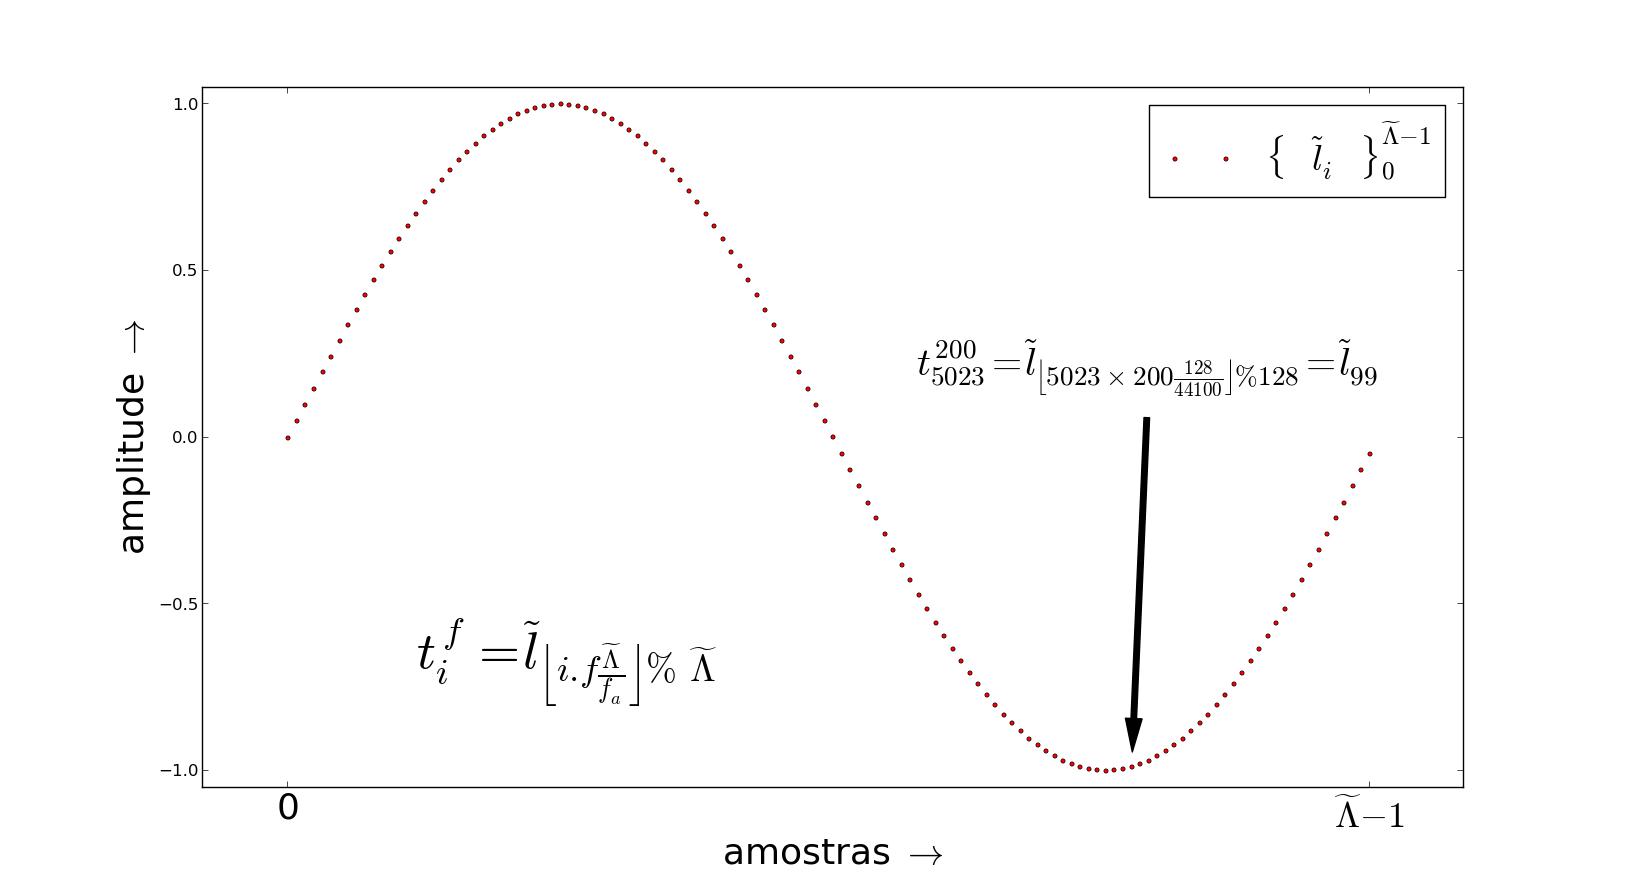
\includegraphics[width=\textwidth]{figuras/lut}
    \caption{Procedimento de busca em tabela (conhecido como \emph{Lookup Table}) para síntese de sons em frequências diferentes a partir de uma única forma de onda em alta resolução.}
        \label{fig:lut}
\end{figure}

Seja $\widetilde{\Lambda}$ o tamanho 
do período e $\widetilde{L_i} = \left\{\, \widetilde{l}_i \,\right\}_0^{\widetilde{\Lambda} -1}$ os elementos $\widetilde{l_i}$ de um
período de onda qualquer (veja equação ~\ref{periodoUnico}). Uma sequência
$T_i^{f,\,\Delta}$ com amostras de um som de frequência $f$ e duração $\Delta$
pode ser obtida a partir de $\widetilde{L_i}$ da seguinte forma:

\begin{equation}\label{eq:lut}
T_i^{f,\,\Delta}=\left\{t_i^f\right\}_0^{\lfloor \, f_a . \Delta \, \rfloor -1} = \left\{ \, \widetilde{l}_{\gamma_i \% \widetilde{\Lambda} }\, \right\}_{0}^{\Lambda-1}\; , \quad \text{onde} \;\; \gamma_i = \left \lfloor i . f \frac{ \widetilde{\Lambda}}{f_a} \right \rfloor  
\end{equation}

Ou seja, com os índices corretos ($\gamma_i\%\widetilde{\Lambda}$)
da LUT, pode-se sintetizar o som em qualquer frequência. 
A figura~\ref{fig:lut} ilustra
o cálculo de uma amostra de $\{t_i\}$ 
a partir de $\left\{\,\widetilde{l}_i\,\right\}$ para uma frequência
de $f=200Hz$, $\widetilde{\Lambda}=128$ e considerada a taxa de amostragem em $f_a=44.1kHz$.
Esta não é uma configuração praticável, como assinalado abaixo, mas possibilita uma
disposição gráfica do procedimento.


O cálculo do inteiro $\gamma_i$ introduz um ruído, 
e este diminui com o aumento de $\widetilde{\Lambda}$.
Para fins de síntese, em $f_a=44.1 kHz$
 o padrão é usar $\widetilde{\Lambda} = 1024$ amostras, pois já não gera ruído
 relevante no espectro audível. O método de arredondamento ou interpolação não é decisivo.\cite{Geiger}

 A expressão que define a variável $\gamma_i$ pode ser compreendida da
 seguinte forma: $i$ é acrescida de $f_a$ a cada $1$ segundo.
 Caso seja dividida pela frequência de amostragem, resulta $\frac{i}{f_a}$,
que é acrescida de $1$ a cada $1$ segundo. Multiplicada pelo comprimento do período, resulta $i \frac{\widetilde{\Lambda}}{f_a}$
 que varre o 
  período em $1$ segundo. Por fim,
 com a frequência $f$, resulta $i . f \frac{\widetilde{\Lambda}}{f_a}$
 que completa $f$ varreduras do período  $\widetilde{\Lambda}$ em $1$ segundo, i.e. a sequência
 resultante apresenta a frequência fundamental $f$.

Importantes considerações: $f$ é qualquer, só há limitantes nas frequências
graves quando o tamanho da tabela $\widetilde{\Lambda}$ não é suficientemente grande para a taxa de amostragem
$f_a$. O procedimento de busca em tabela
é computacionalmente bastante barato, substituindo cálculos por buscas simples (por isso geralmente
é entendido como um processo de otimização). Salvo quando assinalado,
no texto que usará este procedimento para todos os casos cabíveis pois
simplifica as rotinas e é computacionalmente coerente.

O uso de LUTs é bastante difundido nas implementações computacionais
voltadas para música e um uso clássico que explora com ênfase
as LUTs na síntese sonora musical, é a  chamada 
\emph{Wavetable Synthesis} que consiste em várias LUTs utilizadas em 
conjunto através da mixagem para gerar uma nota musical quasi-periódica.~\cite{Cook,Wavetable}.


\subsection{Variações incrementais de frequência e intensidade}\label{subsec:vars}

Segundo a lei de Weber e Fechner, a percepção humana tem uma relação logarítmica com
o estímulo que a causa.\cite{Weber-Fechner} Em outras palavras, um estímulo em progressão exponencial
é percebido como linear.
Por razões didáticas e dado o uso nas AM e FM (veja subseção~\ref{subsec:tvaf}), a variação linear será abordada primeiro.

Em uma nota de duração $\Delta = \frac{\Lambda}{f_a}$, a frequência $f=f_i$ varia de $f_0$ até $f_{\Lambda -1}$
linearmente. Pode-se escrever:

\begin{equation}\label{freqLinear}
F_i=\{f_i\}_0^{\Lambda-1}=\left\{f_0 + (f_{\Lambda-1}-f_0)\frac{i}{\Lambda-1} \right\}_0^{\Lambda-1}
\end{equation}

\begin{equation}\label{indiceLinear}
\Delta_{\gamma_i}=f_i\frac{\widetilde{\Lambda}}{f_a} \quad \Rightarrow \quad \gamma_i=\left \lfloor \sum_{j=0}^{i} f_j\frac{\widetilde{\Lambda}}{f_a} \right \rfloor   =\left \lfloor \sum_{j=0}^{i} \frac{\widetilde{\Lambda}}{f_a} \left [f_0 + (f_{\Lambda-1}-f_0)\frac{j}{\Lambda-1} \right ] \right \rfloor 
\end{equation}

\begin{equation}\label{serieAmostralLin}
\left\{t_i^{\;\overline{f_0,\, f_{\Lambda-1}}}\right\}_0^{\Lambda-1}=\left\{\,\widetilde{l}_{\gamma_i \% \widetilde{\Lambda}}\,\right\}_0^{\Lambda-1}
\end{equation}

Onde $\Delta_{\gamma_i}=f_i\frac{\widetilde{\Lambda}}{f_a}$ é o incremento da LUT entre duas amostras dada a frequência do som na primeira amostra.

Desta forma, pode-se calcular os elementos $t_i^{\;\overline{f_0,f_{\Lambda-1}}}$
com base no período $\left\{\widetilde{l}_i\right\}_0^{\Lambda-1}$.

As equações \ref{freqLinear}, \ref{indiceLinear} e \ref{serieAmostralLin} são relativas à progressão linear
da frequência. Como assinalado para o caso geral, também aqui
uma progressão de frequência
\emph{percebida} como linear segue uma progressão exponencial\footnote{Ou,
dito ainda de outra forma, uma progressão geométrica da frequência
é percebida como uma progressão aritmética de alturas.}.
Pode-se escrever que: $f_i=f_0 . 2^{\frac{i}{\Lambda-1} n_8}$ onde 
$n_8=\log_2\frac{f_{\Lambda-1}}{f_0}$ é o número de oitavas entre $f_0$ e $f_{\Lambda-1}$.
De forma que $f_i=f_0 . 2^{\frac{i}{\Lambda-1}\log_2\frac{f_{\Lambda-1}}{f_0}}=
f_0 . 2^{\log_2\left ( \frac{f_{\Lambda-1}}{f_0} \right )^{\frac{i}{\Lambda-1}}}=
f_0 \left ( \frac{f_{\Lambda-1}}{f_0} \right ) ^{\frac{i}{\Lambda -1}}$. Portanto,
 as equações de transições de frequência
lineares para o ouvido são:

\begin{equation}\label{freqExponencial}
F_i=\{f_i\}_0^{\Lambda-1}=\left\{f_0 \left ( \frac{f_{\Lambda-1}}{f_0} \right ) ^{\frac{i}{\Lambda -1}} \right\}_0^{\Lambda-1}
\end{equation}

\begin{equation}\label{indiceExponencial}
\Delta_{\gamma_i}=f_i\frac{\widetilde{\Lambda}}{f_a} \quad \Rightarrow \quad \gamma_i=\left \lfloor \sum_{j=0}^{i} f_j\frac{\widetilde{\Lambda}}{f_a} \right \rfloor   =\left \lfloor \sum_{j=0}^{i} f_0 \frac{\widetilde{\Lambda}}{f_a} \left ( \frac{f_{\Lambda-1}}{f_0} \right ) ^{\frac{j}{\Lambda -1}} \right \rfloor
\end{equation}

\begin{equation}\label{serieAmostralLog}
\left\{t_i^{\;\overline{f_0,\,f_{\Lambda-1}}}\right\}_0^{\Lambda-1}=\left\{\,\widetilde{l}_{\gamma_i \% \widetilde{\Lambda}}\,\right\}_0^{\Lambda-1}
\end{equation}

\begin{figure}[h!]
    \centering
        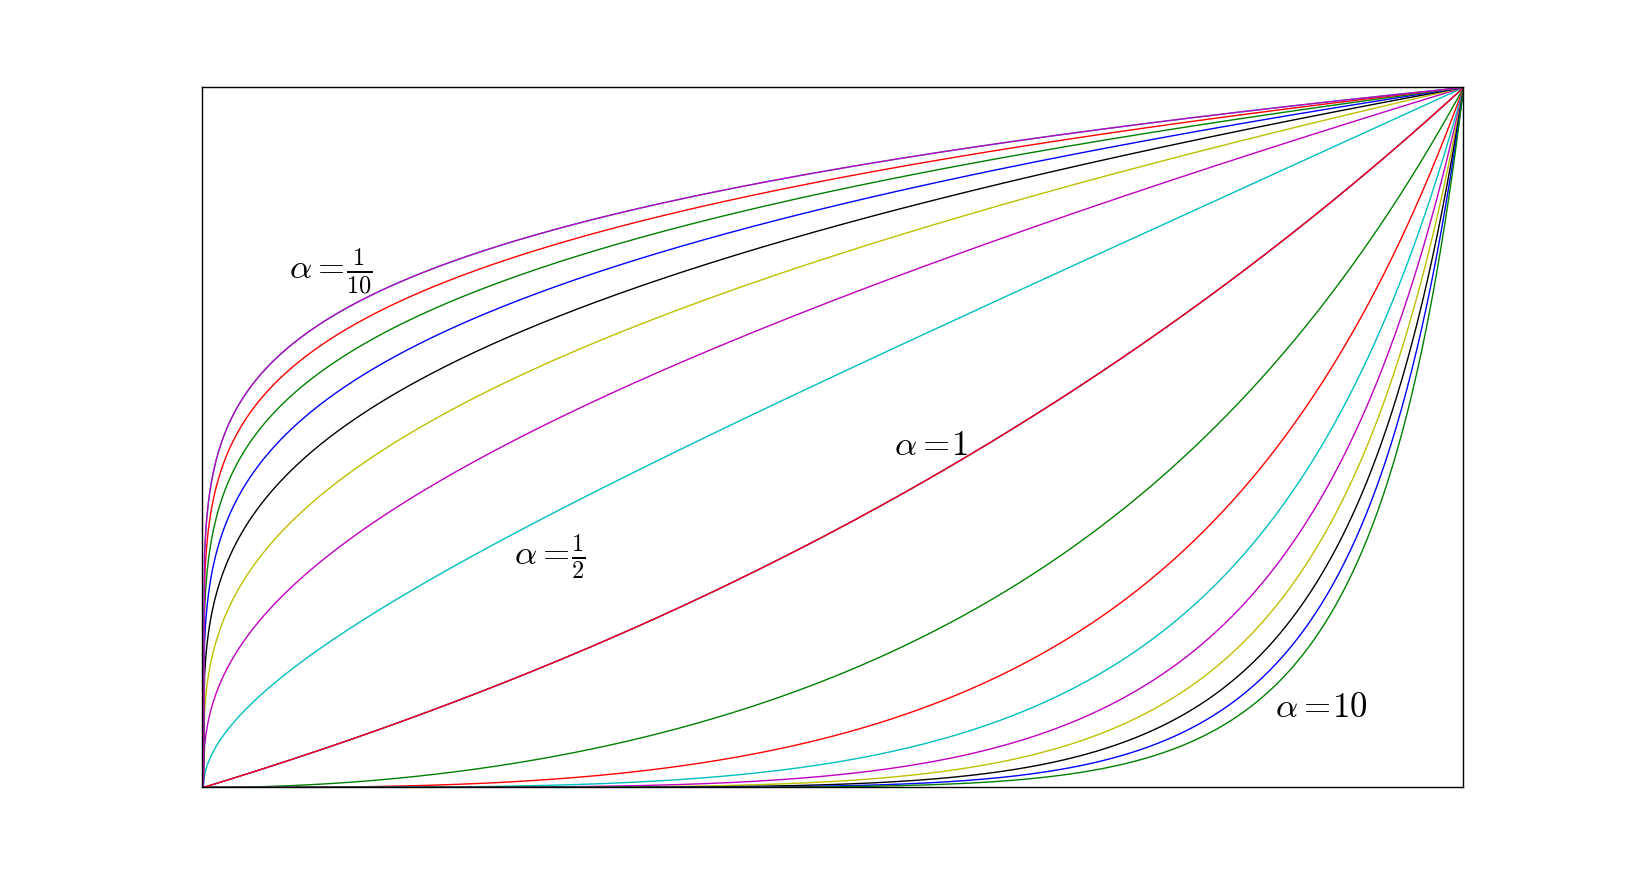
\includegraphics[width=\textwidth]{figuras/transicao}
    \caption{Transições de intensidade para diferentes valores de $\alpha$ (veja equações~\ref{seqAmp} e ~\ref{transAmp}).}
        \label{fig:transicao}
\end{figure}


O termo $\frac{i}{\Lambda-1}$ varre o intervalo $[0,1]$ e pode-se elevá-lo a uma potência
para que o início da transição seja mais suave ou abrupto.
Este procedimento é útil para variações de energia
da onda vibratória para alteração do volume\footnote{A mudança do volume (qualidade psicofísica) ocorre através de diferentes características 
do som, como a reverberação e a concentração de harmônicos agudos, dentre as quais está a energia da onda.
A manipulada com mais facilidade é a energia da onda (veja equação~\ref{eq:potencia}) e esta também pode variar de diferentes formas.
Uma forma mais simples é variar a amplitude através da multiplicação da sequência toda
por um número real. O aumento de energia sem variação de
amplitude é a \emph{compressão sonora}, útil na
produção musical atual.\cite{guillaume}}. Basta multiplicar a sequência original
(seja ela gerada ou pré-estabelecida) pela sequência $a_{\Lambda-1}^{\left( \frac{i}{\Lambda-1} \right )^\alpha}$
onde $\alpha$ é o coeficiente citado e $a_{\Lambda-1}$ é fração da amplitude original que se visa atingir ao final da transição.

Assim, para variações de amplitude:

\begin{equation}\label{seqAmp}
\{a_i\}_0^{\Lambda-1}=\left \{ a_0 \left ( \frac{a_{\Lambda-1}}{a_0} \right )^{\left ( \frac{i}{\Lambda-1} \right )^\alpha} \right \}_0^{\Lambda-1}=\left \{ \left ( {a_{\Lambda-1}} \right )^{\left ( \frac{i}{\Lambda-1} \right )^\alpha} \right \}_0^{\Lambda-1} \text{ com } a_0=1
\end{equation}

\begin{equation}\label{transAmp}
T_i^{'}=T_i \odot A_i = \{t_i . a_i\}_0^{\Lambda-1}=\left \{ t_i . (a_{\Lambda-1} )^{\left ( \frac{i}{\Lambda-1} \right )^\alpha} \right \}_0^{\Lambda-1}
\end{equation}

Pode-se tomar $a_0=1$ para iniciar a nova sequência com a amplitude original e então ir modificando com o decorrer das amostras.
Esta restrição faz com que o termo $a_{\Lambda-1}$ seja a variação da amplitude.
Caso $\alpha=1$, a variação de amplitude segue exatamente a progressão geométrica que caracteriza
a percepção linear. A figura~\ref{fig:transicao} exibe as transições para diferentes valores de $\alpha$ e para a transição entre os valores $1$ e $2$, um ganho de $\approx 6dB$ segundo a equação~\ref{eq:ampVol}.


Algum cuidado é necessário para lidar com $a=0$.
Na equação~\ref{seqAmp}, se $a_0=0$ há divisão por zero e
se $a_{\Lambda-1}=0$, há uma multiplicação por zero. Ambos os casos
tornam o procedimento inútil pois nenhum número diferente de zero pode ser representado como uma proporção com relação ao zero. Pode-se resolver isso escolhendo um número suficientemente pequeno como $-80dB\;\Rightarrow a=10^{\frac{-80}{20}}=10^{-4}$ como o volume mínimo no caso de um
\emph{fade in} ($a_0=10^{-4}$) ou de um \emph{fade out} ($a_{\Lambda-1}=10^{-4}$).


Para uma amplificação linear, mas não linear para a percepção, basta usar uma sequência $\{a_i\}$ adequada:

\begin{equation}\label{seqAmpLin}
a_i=a_0 + (a_{\Lambda-1}-a_0)\frac{i}{\Lambda-1}
\end{equation}

Aqui convém a conversão de decibels para amplitude. Assim, as equações ~\ref{ampDec} e \ref{transAmp}
especificam a transição de $V_{dB}$ decibels:

\begin{equation}\label{seqAmpDB}
T_i^{'}=\left\{ t_i 10^{\frac{V_{dB}}{20}\left( \frac{i}{\Lambda-1} \right)^\alpha} \right\}_0^{\Lambda-1}
\end{equation}

para o caso geral de variações de amplitude segundo a progressão geométrica. Quanto maior o valor de $\alpha$, mais suave é a introdução do som e mais intenso o final da transição. $\alpha>1$ resulta em transições de volume muitas vezes chamadas de \emph{slow fade} enquanto $\alpha<1$ resulta em \emph{fast fade}.\cite{guillaume}

As transições lineares serão usadas para
as sínteses AM e FM e a aplicação das transições
logarítmicas para os tremolos e vibratos.
Uma exploração não oscilatória destas variações
está na montagem musical \emph{Transita para metro},
cujo código está no Apêndice~\ref{ap:transita} e online
na \massa.\cite{MASSA}

\subsection{Aplicação de filtros digitais}\label{subsec:filtros}
Esta subseção limita-se a uma descrição
do processamento das sequências, por convolução
e equação a diferenças, e em aplicações
imediatas, pois a complexidade facilmente
foge ao escopo\footnote{A elaboração de filtros
constitui uma área reconhecidamente complexa, com literatura
e pacotes de software dedicados. 
Recomendamos ao leitor
interessado uma visita à nossa bibliografia.\cite{Openheim,smith}}. A aplicação de filtros pode
ser parte constituinte da síntese ou feita posteriormente
como parte dos processos tipicamente chamados de tratamento sonoro.

\begin{itemize}

\item  Convolução e filtros de resposta ao impulso finita (FIR)

\begin{figure}[h!]
    \centering
        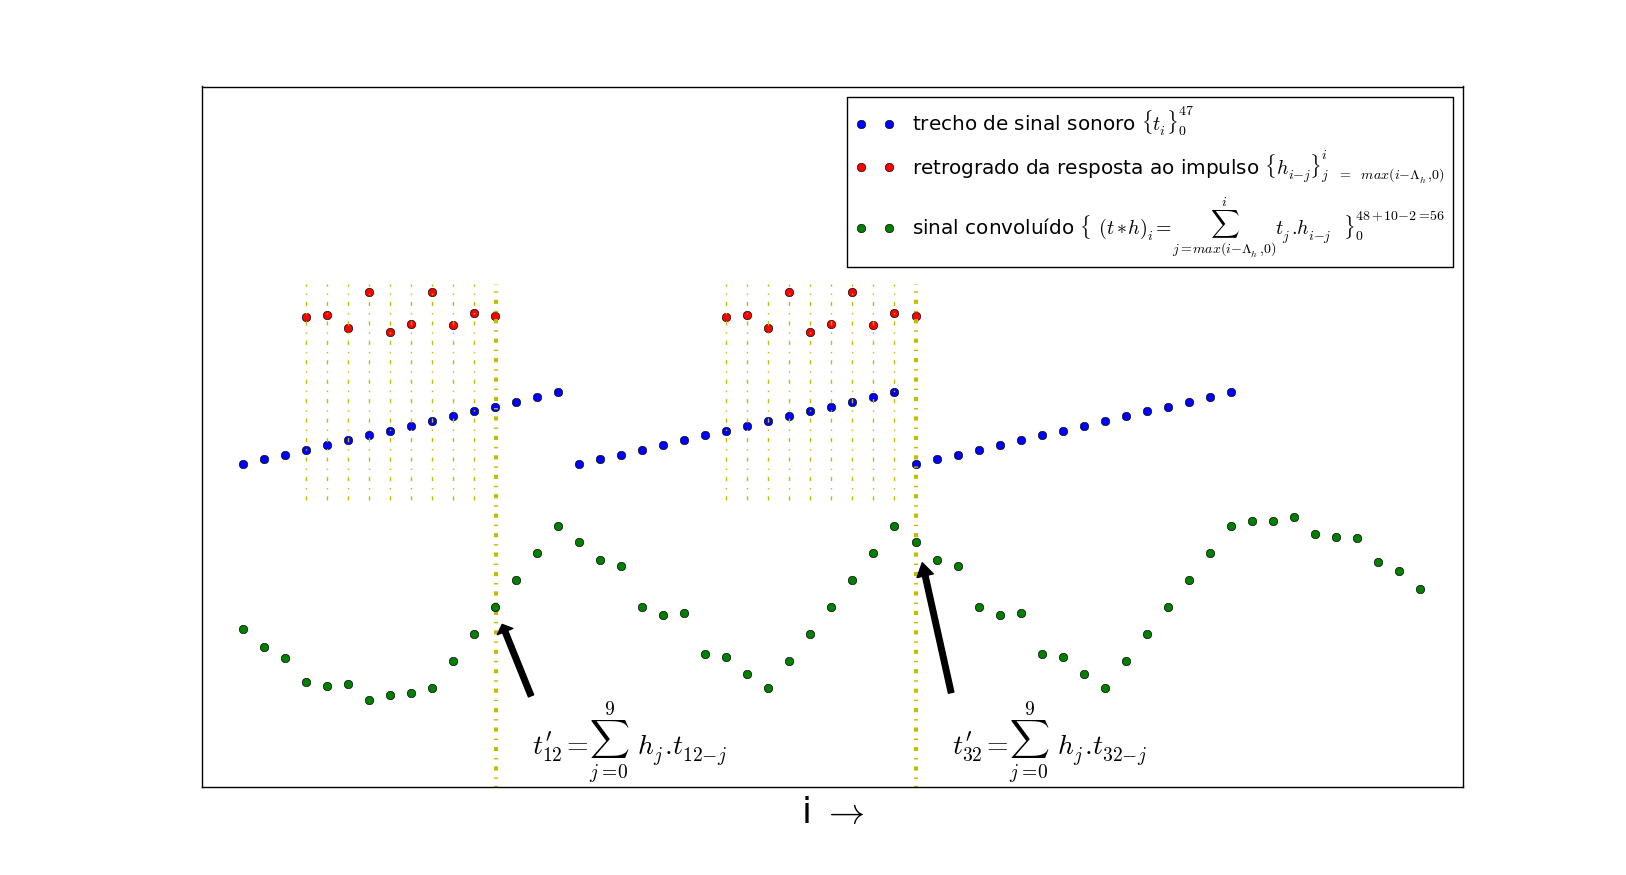
\includegraphics[width=\textwidth]{figuras/convolucao______}
    \caption{Interpretação gráfica da convolução. Cada amostra resultante é a soma das amostras anteriores de um sinal uma a uma multiplicadas pelas amostras retrógradas do outro sinal.}
        \label{fig:conv}
\end{figure}

Os filtros aplicados por convolução são conhecidos
pela sua sigla FIR (do inglês Finite Impulse Response)
e são caracterizados por possuirem uma representação amostral
finita no tempo. Esta representação amostral é chamada
de 'resposta ao impulso' $\{h_i\}$. Os filtros FIR são aplicados 
no domínio temporal ao som
digitalizado pela convolução do som com a 
resposta ao impulso do filtro\footnote{Pode-se aplicar o filtro do domínio espectral através da multiplicação das transformadas de Fourier de ambos o som e a resposta ao impulso, e então realizada a transformada inversa de Fourier do espectro resultante.\cite{Openheim}}. Para os fins deste trabalho, a
convolução fica definida como:

\begin{equation}\label{eq:conv}
\begin{split}
\left\{t_i'\right\}_0^{\Lambda_t+\Lambda_h-2\; = \;\Lambda_{t\, '}-1} =\{(T_j*H_j)_i\}_0^{\Lambda_{t \, '}-1} & =\left \{ \sum_{j=0}^{min(\Lambda_h-1,i)}h_{j} . t_{i-j} \right \}_0^{\Lambda_{t\, '}-1} \\
    & =\left \{ \sum_{j=max(i+1-\Lambda_h,0)}^{i}t_j . h_{i-j} \right \}_0^{\Lambda_{t\, '}-1}
\end{split}
\end{equation}

Onde $t_i=0$ para as
amostras não definidas de antemão.
Ou seja, o som $\{t_i'\}$ resultante da convolução de $\{t_i\}$ com a resposta ao impulso $\{h_i\}$
tem cada i-ésima amostra $t_i$ substituída pela soma de suas últimas $\Lambda_h$ amostras $\{t_{i-j}\}_{j=0}^{\Lambda_h-1}$
multiplicadas uma a uma pelas amostras da resposta ao impulso $\{h_i\}_0^{\Lambda_h-1}$. Este
procedimento está ilustrado na figura~\ref{fig:conv}, onde a resposta ao impulso $\{h_i\}$
é percorrida na forma retrógrada e
$t_{12}'$ e $t_{32}'$ são duas amostras calculadas
pela convolução $(T_j*H_j)_i=t_i'$. O sinal resultante possui
sempre o tamanho $\Lambda_t+\Lambda_h -1=\Lambda_{t'}$.


Com este procedimento pode-se aplicar reverberadores, equalizadores, delays
e vários outros tipos de filtros para fins de tratamento sonoro ou
efeitos musicais/artísticos.
 
A resposta ao impulso pode provir de medições
físicas ou da síntese. Uma resposta 
ao impulso para a aplicação
de reverberação pode resultar da gravação sonora em um ambiente ao disparar
um estalo que se assemelhe a um impulso ou 
de uma varredura em senoide, que transformada se aproxima
da resposta em frequência.
Ambas são respostas ao impulso
que, convoluídas com a sequência sonora, resultam na própria sequência
com uma reverberação que se assemelha àquela do ambiente 
em que ocorreu a medição.\cite{Cook}

A transformada inversa
de Fourier de uma envoltória par e real é uma
resposta ao impulso de um FIR. Este realiza
uma filtragem em frequência com a envoltória.
Quanto maior o número de amostras maior
a resolução da envoltória e também 
o processamento computacional, pois a convolução é cara.

Uma propriedade importante é o deslocamento temporal causado pela convolução com o impulso deslocado. Embora caro computacionalmente, 
pode-se criar linhas de \emph{delays} através da convolução do som com uma resposta ao impulso que possui um impulso
para cada reincidência do som.
Na figura~\ref{fig:delays}
pode-se observar o deslocamento causado pela convolução
com o impulso. Dependendo da densidade dos impulsos, o resultado
é de caráter rítmico (20 impulsos por segundo ou menos) ou de amálgama
sonoro (20-40 impulsos por segundo ou mais). Neste último caso,
ocorrem processos tipicamente vinculados à síntese granular, delays, reverbs e equalizações.

\begin{figure}[h!]
    \centering
        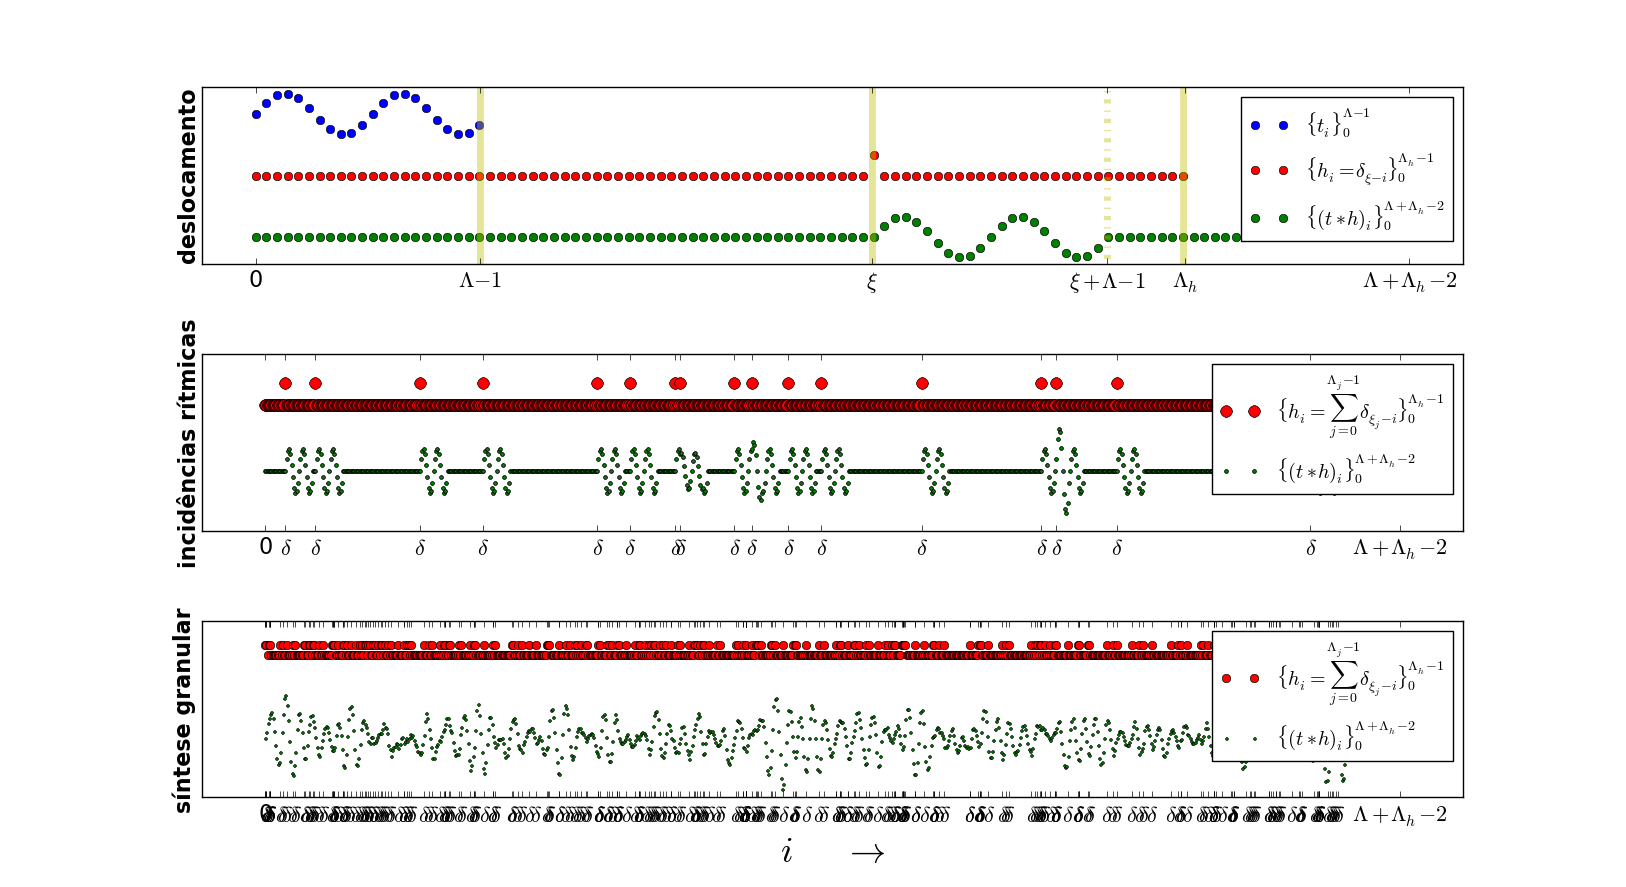
\includegraphics[width=\textwidth]{figuras/delays__}
    \caption{Convolução com o impulso: deslocamento (a), linhas de delays (b) e síntese granular~(c). Dispostos em ordem crescente de densidade de pulsos.}
        \label{fig:delays}
\end{figure}


\item Filtros de resposta ao impulso infinita (IIR)

Esta classe de filtros é
conhecida pela sigla IIR (do inglês Infinite Impulse Response)
e é caracterizada por possuir uma representação temporal
infinita, i.e. a resposta ao impulso não converge para zero.
Sua aplicação é usualmente feita pela equação:

\begin{equation}\label{eq:diferencas}
t_i' = \frac{1}{b_0}\left ( \sum_{j=0}^Ja_j . t_{i-j} + \sum_{k=1}^Kb_k . t_{i-k}' \right )
\end{equation}

com $b_0=1$ na grande maioria dos casos pois pode-se normalizar as variáveis:
$a_j'=\frac{a_j}{b_0}$ e $b_k'=\frac{b_k}{b_0} \Rightarrow b_0' = 1$.
A equação~\ref{eq:diferencas} é chamada 'equação a diferenças' por exibir as amostras resultantes $\left\{t_i'\right\}$
através das diferenças entre as amostras originais $\{t_i\}$ e as amostras resultantes anteriores $\left\{t_{i-k}'\right\}$.

Existem
diversos métodos e ferrametas para a elaboração de filtros IIR
e segue abaixo uma seleção com fins didáticos e para consulta futura por
utilidade.
São filtros bem comportados e cujas
filtragens estão na figura~\ref{fig:iir}.

No caso dos filtros de ordem simples, a frequência de corte $f_c$ é onde 
o filtro realiza uma atenuação de $-3dB \approx 0.707 $ da amplitude original.
No caso dos filtros passa e rejeita banda, esta mesma atenuação é
resultado de duas especificações: $f_c$ (neste caso mais bem compreendida como 'frequência central') e a largura de banda $bw$,
em ambas as frequências $f_c \pm bw$ há uma atenuação de $\approx 0.707$ da amplitude original.
Existe amplificação do som no caso dos filtros passa e rejeita banda quando a frequência
de corte é baixa e a largura de banda é grande o suficiente. Nos agudos, estes filtros apresentam
somente um desvio do perfil esperado, expandindo a envoltória para o lado grave da banda em
evidência.

Para filtros cujas respostas em frequência possuem outras envoltórias (para o módulo),
pode-se realizar cascatas destes filtros aplicando-os sucessivamente.
Outra possibilidade é utilizar alguma receita de filtro
biquad\footnote{Abreviação
de 'biquadrado' pois sua função de transferência possui dois polos e dois zeros, i.e. sua
forma normal consiste em dois polinômios quadráticos formando uma fração:
$\mathbb{H}(z)=\frac{a_0+a_1.z^{-1}+a_2.x^{-2}}{1- b_1.z^{-1} -b_2 . z^{-2}}$.}
ou rotinas para cálculo de coeficientes
de filtros Chebichev\footnote{Filtros Butterworth e Elípticos podem
ser considerados como casos específicos dos Filtros do tipo Chebichev.\cite{Openheim,smith}}.
Ambas as possibilidades são exploradas
por títulos em nossas referências, em especial~\cite{JOSFM,smith} e a coleção de filtros da comunidade \emph{Music-DSP}, da Universiade de Columbia.\cite{music-dsp,Openheim}

\end{itemize}

\begin{enumerate}
\item Passa-baixas de polo simples com módulo da resposta em frequência no canto superior esquerdo da figura~\ref{fig:iir}. A fórmula geral tem
por referência da frequência de corte $f_c \in (0,\frac{1}{2})$,
fração da frequência de amostragem $f_a$
em que há aproximadamente uma atenuação de $3dB$.
Os coeficientes do filtro IIR
$a_0$ e $b_1$ 
são dados através da variável intermediária $x \in [e^{-\pi},1]$:

\begin{figure}[h!]
    \centering
        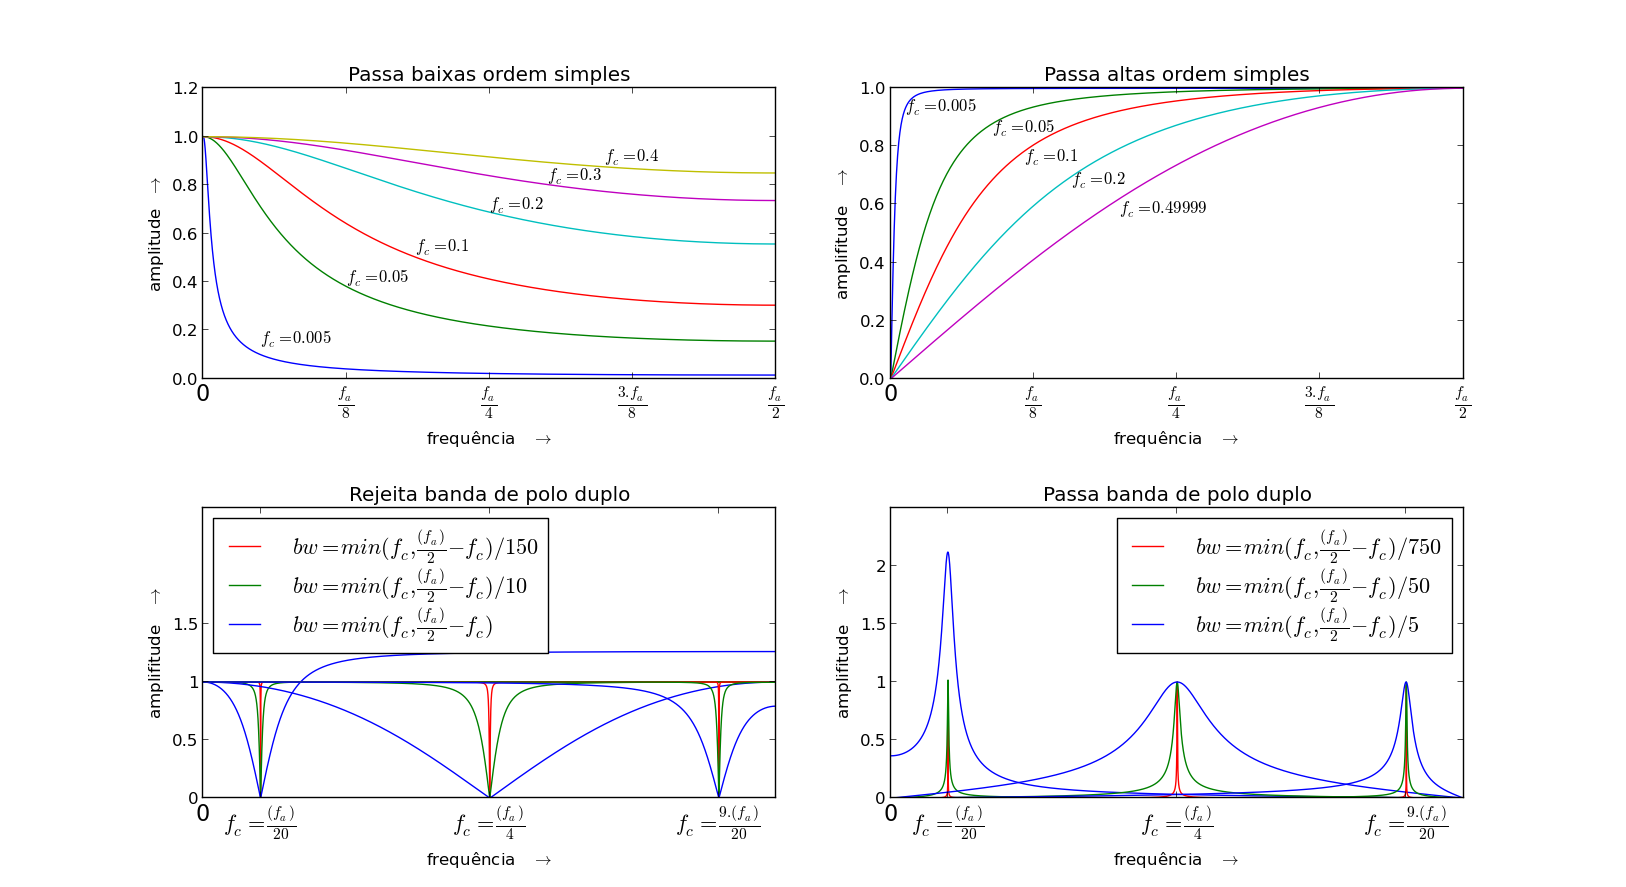
\includegraphics[width=\textwidth]{figuras/iir___}
    \caption{Módulos da resposta em frequência (a), (b), (c) e (d) respectivamente dos filtros IIR das equações \ref{eq:passa-baixas}, \ref{eq:passa-altas}, \ref{eq:passa-banda} e \ref{eq:rejeita-banda} para diferentes frequências de corte, frequências centrais e larguras de banda.}
        \label{fig:iir}
\end{figure}


\begin{equation}\label{eq:passa-baixas}
\begin{split}
x & =e^{-2\pi f_c} \\
a_0 & =  1-x \\
b_1 & =  x
\end{split}
\end{equation}

\item Passa-altas de polo simples com o módulo da resposta em frequência no canto superior direito da figura~\ref{fig:iir}. A fórmula geral,
com frequência de corte $f_c \in (0,\frac{1}{2})$, é calculada através da variável
intermediária $x \in [e^{-\pi},1]$:


\begin{equation}\label{eq:passa-altas}
\begin{split}
x & =e^{-2\pi f_c} \\
a_0 & =  \frac{x+1}{2} \\
a_1 & =  -\frac{x+1}{2} \\
b_1 & =  x
\end{split}
\end{equation}


%\item Passa-banda
%\item Rejeita-banda
\item Nó (\emph{notch filter}). Este filtro é parametrizado
pela frequência central\footnote{ Atenção com a frequência de corte também $f_c$ nos filtros passa baixas e passa altas.} $f_c$
e a largura de banda $bw$
- $f_c \pm bw$, que resultam em $0.707$ da amplitude, i.e. atenuação de $3dB$ -
ambos dados como frações de $f_a$, portanto $f,\; bw \in (0,0.5)$.

Por facilidade, sejam as variáveis auxiliares $K$ e $R$:

\begin{equation}\label{eq:varAux}
\begin{split}
R & = 1 - 3bw \\
K & = \frac{1-2R\cos(2\pi f_c) + R^2}{2 - 2 \cos (2 \pi f_c)}
\end{split}
\end{equation}

O filtro passa banda do canto inferior esquerdo da figura~\ref{fig:iir}
possui os seguintes coeficientes para a equação~\ref{eq:diferencas}:

\begin{equation}\label{eq:passa-banda}
\begin{split}
a_0 & =  1 - K \\
a_1 & =  2(K-R)\cos (2\pi f_c) \\
a_2 & =  R^2-K \\
b_1 & =  2R \cos (2\pi f_c) \\
b_2 & =  -R^2
\end{split}
\end{equation}

Os coeficientes do filtro rejeita banda são:

\begin{equation}\label{eq:rejeita-banda}
\begin{split}
a_0 & =  K \\
a_1 & =  -2K\cos (2\pi f_c) \\
a_2 & =  K \\
b_1 & =  2R \cos (2\pi f_c) \\
b_2 & =  -R^2
\end{split}
\end{equation}

com o módulo de sua resposta em frequência 
disposto na parte inferior esquerda da figura~\ref{fig:iir}.

%\item Biquad: pela especificação de uma frequência central, da qualidade
%e da intensidade do filtro, este filtro é simples e usual para áudio,
%permitindo ajustes mais finos. Diversas receitas podem ser encontradas
%na literatura, recomendamos especialmente as diferentes especificações
%em ~\ref{musicDSP} e ~\ref{dspguide}.

\end{enumerate}

\subsection{Ruídos}\label{subsec:ruidos}
De forma geral, os sons sem altura definida 
são chamados ruídos.\cite{Lacerda}
Estes são constituintes importantes dos sons musicais de altura definida,
como os ruídos presentes nas notas do piano, do violino, etc. Além disso, os instrumentos
de percussão, em grande parte, não possuem altura definida e seus sons
são em geral compreendidos como ruídos.\cite{Roederer} Na música eletrônica, incluindo
a eletroacústica e gêneros de pista de dança, os ruídos possuem usos diversificados e comumente
característicos do estilo musical.\cite{Cook}

A ausência de uma altura definida é fruto da ausência de uma organização harmônica perceptível nas componentes senoidais que formam o som. Assim,
são incontáveis as possibilidades de gerar ruídos.
A utilização
de valores aleatórios para a geração da sequência sonora $T_i$
é um método atraente,
mas os resultados não são tão úteis, tendendo geralmente ao ruído branco.\cite{Cook}

Outra possibilidade é a geração de ruído através do espectro desejado, a partir
do qual executamos a transformada inversa de Fourier.
A distribuição espectral deve ser feita com cuidado 
pois caso se utilize a mesma fase,
ou fases com forte correlação, 
o som sintetizado possuirá energia bastante concentrada
em alguns trechos de sua duração.


\begin{figure}[htpq!]
    \centering
        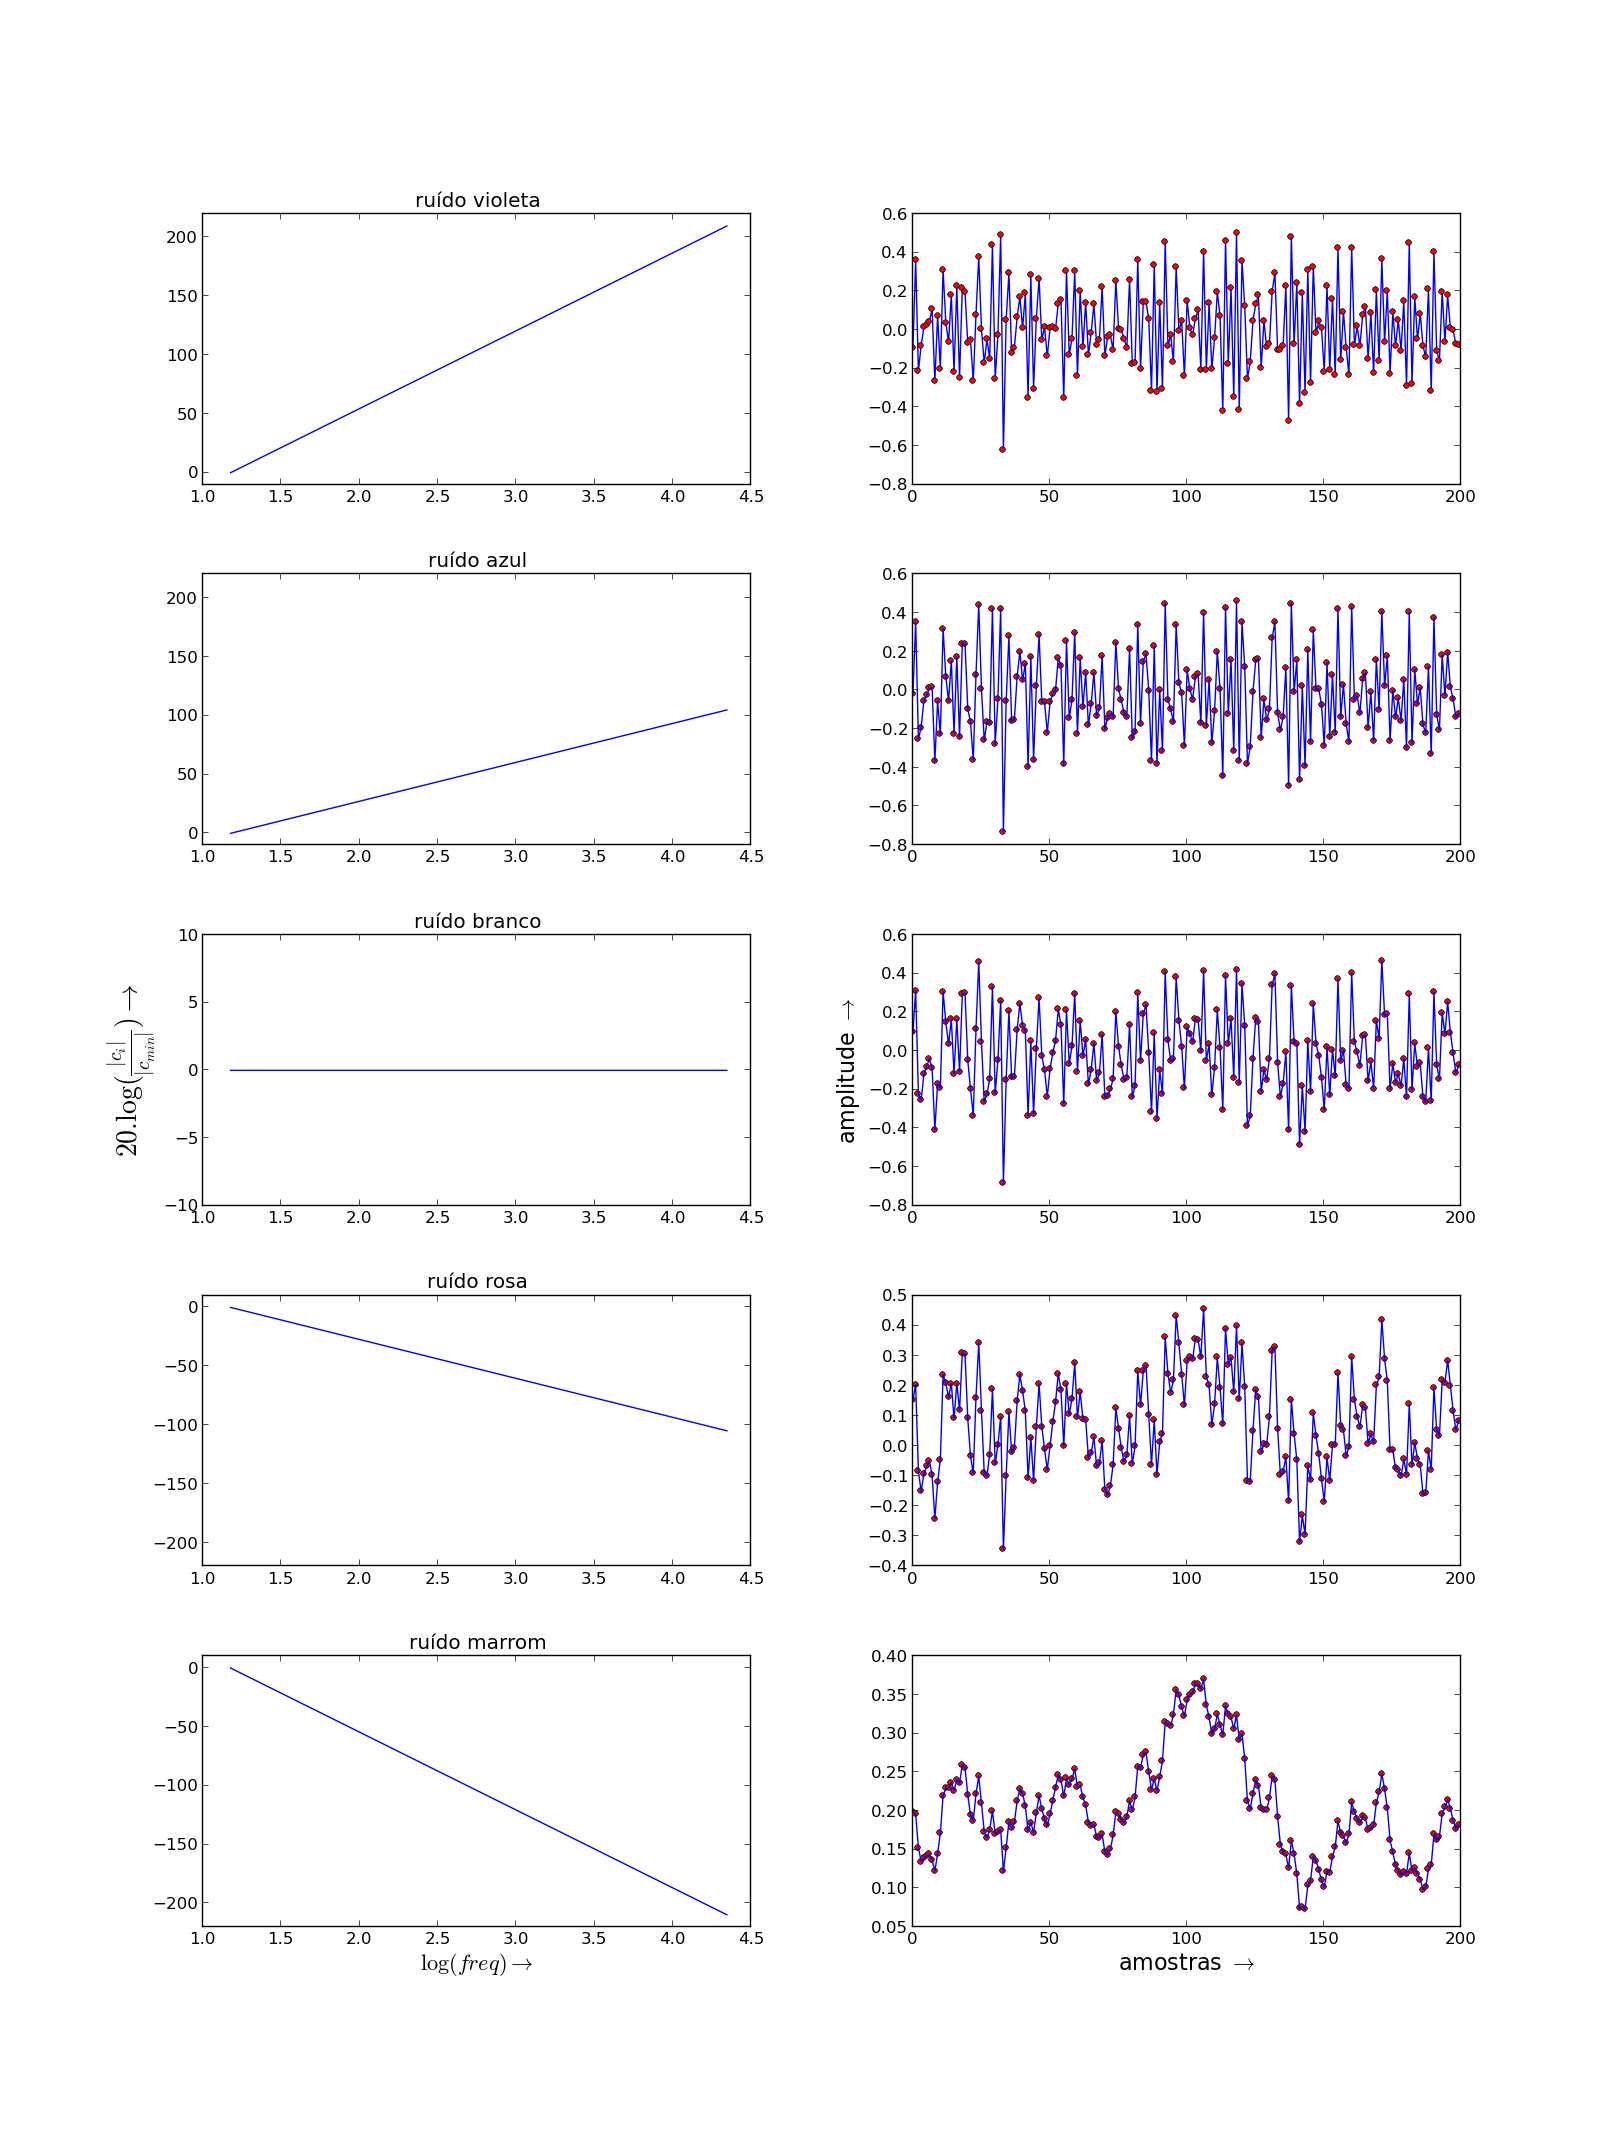
\includegraphics[width=\textwidth]{figuras/ruidos___}
    \caption{Ruídos coloridos realizados através das equações~\ref{eq:branco}, \ref{eq:rosa}, \ref{eq:marrom}, \ref{eq:azul}, \ref{eq:violeta}: espectros e ondas sonoras resultantes.}
        \label{fig:ruidos}
\end{figure}


Abaixo elencamos alguns ruídos de espectro estático. São chamados \emph{coloridos} por terem sido associados a cores. 
A figura~\ref{fig:ruidos} mostra lado a lado o perfil espectral e
a sequência sonora. Os ruídos foram gerados com a mesma fase, então
pode-se observar o resultado das contribuições em diferentes regiões do espectro.

\begin{itemize}

\item O ruído branco deve seu nome por possuir energia distribuída
igualmente por todas as frequências. Pode-se realizar
o ruído branco com a transformada inversa dos seguintes coeficientes:


\begin{equation}\label{eq:branco}
\begin{split}
c_0 & =0 \quad \text{pois evita-se bias} \\
c_i & =e^{j.x}\;,\;\; j^2=-1 \;, \;\; x \; \text{randômico} \; \in \; [0,2\pi]\;,\;\; i \; \in \; \left[1, \, \frac{\Lambda}{2}-1\right] \\
c_{\Lambda/2} & = 1 \quad\quad \text{(se $\Lambda$ par)}\\ 
c_i & = c_{\Lambda - i}^*\;,\;\; \text{para}\;  i \; > \;  \frac{\Lambda}{2}
\end{split}
\end{equation}

O valor de $c_i$ calculado pela exponencial é apenas um artifício para resultar em módulo unitário e fase aleatória.
Já $c_{\Lambda/2}$ é sempre puramente real (como vimos na seção anterior).

\item O ruído rosa possui uma queda de $3dB$ por oitava. Este ruído é muito usual no teste de equipamentos e montagens de aparelhos além de presença destacada na natureza~\cite{Roederer}. 

\begin{equation}\label{eq:rosa}
\begin{split}
f_{\text{min}} & \approx 15 Hz \\
f_i & = i \frac{f_a}{\Lambda} \;, \;\; \quad i \;\leq\; \frac{\Lambda}{2},\;\; i\;\in\;\mathbb{N}  \\
\alpha_i & = \left(10^{-\frac{3}{20}}\right)^{\log _2 \left ( \frac{f_i}{f_{\text{min}}} \right )}  \\
c_i & =0\;,\;\; \forall \; i \; : f_i<f_{\text{min}} \\
c_i & =e^{j.x} . \alpha_i\;,\;\; j^2=-1 \;, \;\;\  x \;\; \text{randômico} \; \in \; [0,2\pi]\;,\;\; \forall \; i \; : f_{\text{min}} \le f_i < f_{\lceil \Lambda/2-1 \rceil}  \\
c_{\Lambda/2} & = \alpha_{\Lambda/2} \quad\quad \text{(se $\Lambda$ par)}\\ 
c_i & = c_{\Lambda - i}^*\;,\;\; \text{para}\;  i \; > \;  \Lambda/2
\end{split}
\end{equation}

A frequência mínima $f_{\text{min}}$ pode ser escolhida com base no limite da audição, pois não se escuta como altura uma componente sonora cuja frequência esteja abaixo de $\approx\; 20Hz$.

Os ruídos restantes podem ser feitos com base no procedimento descrito para 
o ruído rosa, bastando que modificar detalhes, em especial a equação que define $\alpha_i$.

\item O ruído marrom deve seu nome a Robert Brown, que descreveu o movimento browniano.
Embora esta origem seja um tanto díspar do que pode-se considerar motivo para uma associação com a cor marrom, o ruído sonoro ficou consagrado com este nome. De qualquer forma, é bastante comum declarar satisfatória a associação do ruído com a cor marrom, uma vez que os ruídos branco e rosa são mais estridentes e relacionados a cores mais intensas~\cite{Cook,guillaume}.

O que caracteriza este ruído é a queda de $6dB$ por oitava. Desta forma, $\alpha_i$ 
no conjunto \ref{eq:rosa} fica:

\begin{equation}\label{eq:marrom}
\alpha_i=(10^{-\frac{6}{20}})^{\log _2 \left( \frac{f_i}{f_{\text{min}}} \right )}
\end{equation}

\item No ruído azul há ganho de $3dB$ por oitava em uma banda limitada
pela frequência mínima $f_{\text{min}}$ e a frequência
máxima $f_{\text{máx}}$. Assim, também com base no conjunto de equações \ref{eq:rosa}:

\begin{equation}\label{eq:azul}
\begin{split}
\alpha_i & = (10^{\frac{3}{20}})^{\log _2 \left ( \frac{f_i}{f_{\text{min}}} \right )} \\
c_i & =0\;,\;\; \forall \; i \; : f_i<f_{\text{min}} \;\; \text{ou} \;\; f_i>f_{\text{máx}} \\
\end{split}
\end{equation}

\item O ruído violeta é similar ao ruído azul, mas o ganho é de $6dB$ por oitava:

\begin{equation}\label{eq:violeta}
\alpha_i = (10^{\frac{6}{20}})^{\log _2 \left ( \frac{f_i}{f_{\text{min}}} \right )} \;\;, \quad f_{\text{min}} \approx 15 Hz \\
\end{equation}

\item O ruído preto possui perdas maiores que $6dB$ por oitava, assim:

\begin{equation}\label{eq:preto}
\alpha_i=(10^{-\frac{\beta}{20}})^{\log _2 \left( \frac{f_i}{f_{\text{min}}} \right )}\;\;, \quad \beta > 6
\end{equation}



\item O ruído cinza é definido como
um ruído branco sujeito a uma das curvas iso-audíveis. Estas curvas são resultados
experimentais e necessárias para a obtenção de $\alpha_i$. Uma implementação da ISO 226, a última revisão destas curvas, está na toolbox \massa.\cite{MASSA}

\end{itemize}

Foram expostos somente ruídos com espectro estático. Existem classificações
de ruídos com variações do espectro no decorrer do tempo. Existem também ruídos que
são fundamentalmente transientes, como os clicks e os chirps. O primeiro é modelado
facilmente por um impulso relativamente isolado, enquanto o segundo não é um ruído, mas uma varredura rápida de 
alguma banda de frequência.\cite{Cook}

Os ruídos das equações \ref{eq:branco}, \ref{eq:rosa}, \ref{eq:marrom},
\ref{eq:azul}, \ref{eq:violeta} estão na figura \ref{fig:ruidos}. Os espectros foram feitos com a mesma fase em cada coeficiente de mesma frequência, de forma que
se pode observar a contribuição dos harmônicos agudos e
das frequências graves.


\subsection{Tremolo e vibrato, AM e FM}\label{subsec:tvaf}

O vibrato é uma variação periódica de altura (frequência) e 
o tremolo é uma variação periódica de volume (intensidade).\footnote{Alguns instrumentos e contextos musicais usam nomenclaturas diferentes. Por exemplo, no piano, o chamado tremolo é um vibrato e um tremolo segundo a classificação aqui utilizada. As definições presentes neste trabalho tem por base uma literatura mais abrangente do que a utilizada para um único instrumento, prática ou tradição musical e comum em contextos de teoria musical e musica eletrônica.\cite{Lacerda,Harmonia}}
Para o caso geral, o vibrato é descrito da seguinte forma:


\begin{equation}\label{vbrGamma}
\gamma_i'=\left \lfloor i f' \frac{\widetilde{\Lambda}_M}{f_a} \right \rfloor
\end{equation}

\begin{equation}\label{vbrAux}
t_i'=\widetilde{m}_{\gamma_i' \;\% \widetilde{\Lambda}_M}
\end{equation}

\begin{equation}\label{vbrF}
f_i=f \left ( \frac{f + \mu }{f} \right )^{t_i'}=f . 2^{t_i'\frac{\nu}{12}}
\end{equation}

\begin{equation}\label{vbrGamma2}
\Delta_{\gamma_i}=f_i\frac{\widetilde{\Lambda}}{f_a} \quad \Rightarrow \quad \gamma_i = \left \lfloor \sum_{j=0}^{i} f_j \frac{\widetilde{\Lambda}}{f_a} \right \rfloor = \left \lfloor \sum_{j=0}^{i} \frac{\widetilde{\Lambda}}{f_a}f \left ( \frac{f + \mu }{f} \right )^{t_j'}  \right \rfloor= \left \lfloor \sum_{j=0}^{i} \frac{\widetilde{\Lambda}}{f_a}f . 2^{t_j'\frac{\nu}{12}}  \right \rfloor
\end{equation}

\begin{equation}\label{vbrT}
T_i^{f, vbr(f',\,\nu)}=\left\{ t_i^{f,vbr(f',\,\nu)} \right\}_0^{\Lambda-1}=\left\{ \widetilde{l}_{\gamma_i \%\; \widetilde{\Lambda} } \right\}_0^{\Lambda-1}
\end{equation}


\begin{figure}[h!]
    \centering
        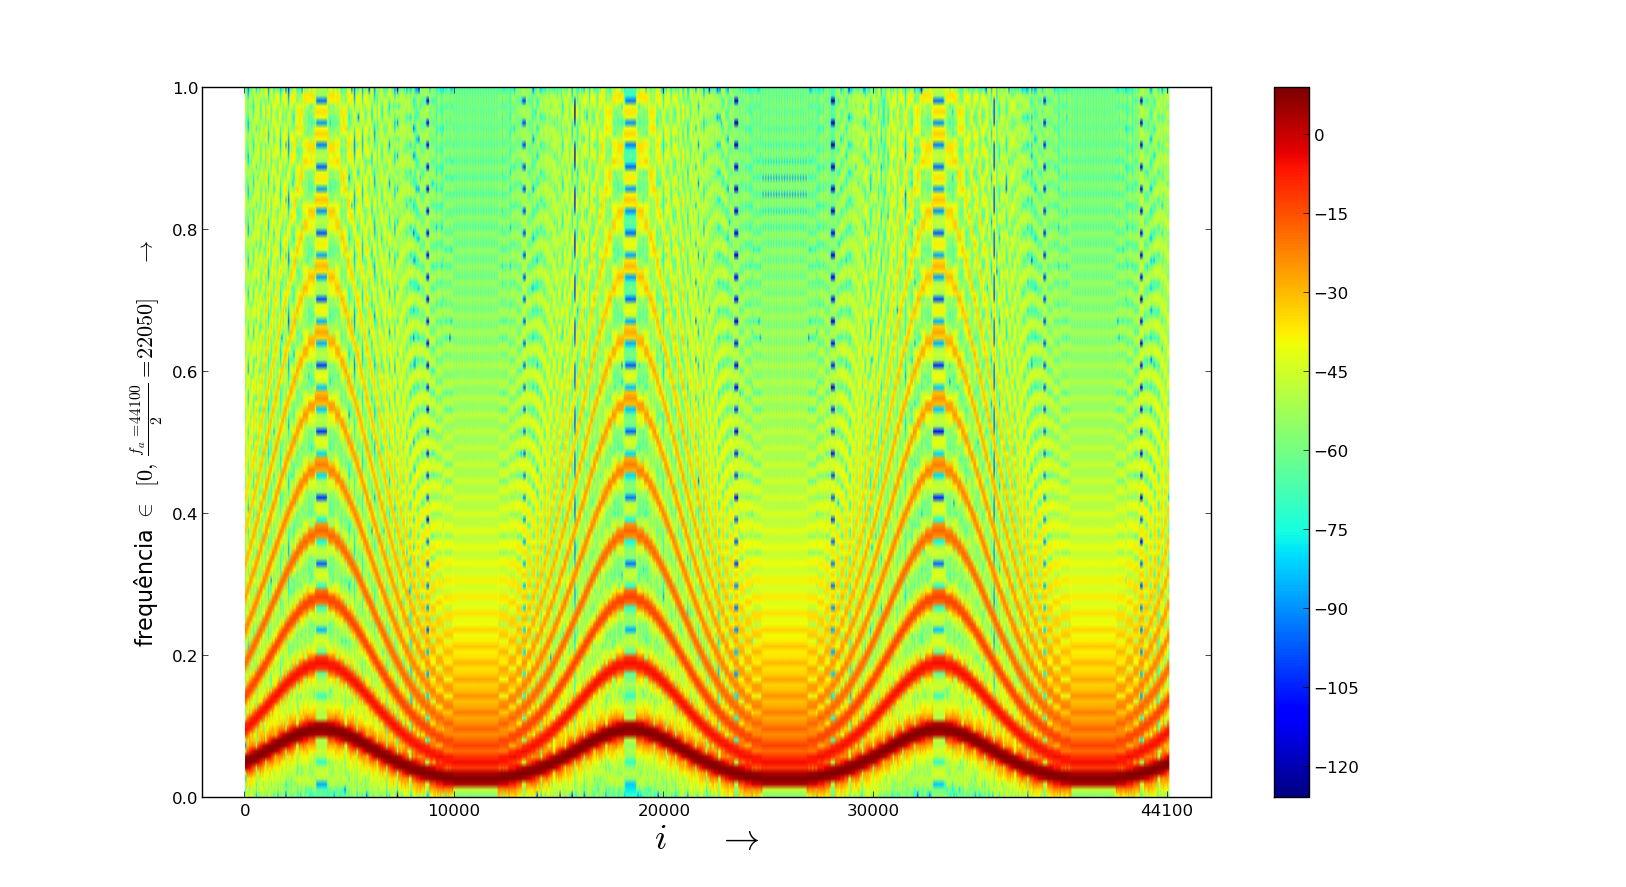
\includegraphics[width=\textwidth]{figuras/vibrato___}
    \caption{Espectrograma de um som com vibrato senoidal de $3Hz$ e profundidade de uma oitava em uma dente de serra de $1000Hz$ (considerada $f_a=44.1kHz$).}
        \label{fig:vibrato}
\end{figure}

Para a correta realização do vibrato, é importante atenção para as duas tabelas e sequências.
A tabela $\widetilde{M}_i$ de tamanho $\widetilde{\Lambda}_M$ e a sequência de índices $\gamma_i'$ formam a sequência $t_i'$
 que é o padrão da oscilação da frequência enquanto
a tabela $\widetilde{L}_i$ de tamanho $\widetilde{\Lambda}$ e a sequência de índices $\gamma_i$ formam $t_i$ que é o som em si.
As variáveis $\mu$ e $\nu$ quantificam a intensidade do vibrato: $\mu$ é uma medida direta da quantidade
de Herz envolvidos no limite superior da oscilação e $\nu$ é a medida direta de semitons envolvidos na oscilação ($2\nu$ é o número de semitons entre os picos superiores e inferiores de oscilação da frequência do som $\{t_i\}$ causada pelo vibrato).
É conveniente $\nu=\log_{2}\frac{f+\mu}{f} $ neste caso pois o aumento máximo de frequência
não equivale à diminuição máxima, mas a variação de semitons se mantém.

A Figura \ref{fig:vibrato} é o espectrograma de um vibrato artificial de uma nota em
$1000Hz$ (entre um si e um dó) e cujo desvio da frequência atinge uma oitava
para cima e para baixo. Qualquer forma de onda pode
ser utilizada para gerar o som e o padrão de oscilação do vibrato
em quaisquer frequência de oscilação e desvio de altura envolvidos\footnote{O desvio de altura
é chamado profundidade do vibrato e é geralmetne dado por conveniência em semitons ou cents.}. Estas oscilações com formas precisas e amplitudes arbitrárias não são praticáveis em instrumentos musicais tradicionais, introduzindo novidade nas possibilidades artísticas.

O caso do tremolo é semelhante: $f'$, $\gamma_i'$ e $t_i'$ permanecem os mesmos.
A sequência de amplitudes a serem multiplicadas pela sequência original $t_i$ fica:

\begin{equation}\label{trA}
a_i=10^{\frac{V_{dB}}{20}t_i' } = a_{\text{máx}}^{t_i'}
\end{equation}

\begin{equation}\label{trT}
T_i^{tr(f')}=\left \{ t_i^{tr(f')} \right \}_0^{\Lambda-1}=\{ t_i . a_i \}_0^{\Lambda-1}=\left \{t_i .10^{t_i' \frac{V_{dB}}{20}}    \right \}_0^{\Lambda-1}=\left\{t_i . a_{\text{máx}}^{t_i'} \right\}_0^{\Lambda-1}
\end{equation}

Onde $V_{dB}$ é a profundidade da oscilação em decibels do tremolo e $a_{\text{máx}}=10^{\frac{V_{dB}}{20}}$
 é o ganho máximo de amplitude envolvido.
A medição em decibels é pertinente pois o aumento máximo de amplitude
não equivale à diminuição máxima relacionada, enquanto a diferença em decibels se mantém.

A figura~\ref{fig:tremolo} mostra a amplitude das sequências $\{a_i\}_0^{\Lambda-1}$ e $\{t_i'\}_0^{\Lambda-1}$
para três oscilações de um tremolo com forma da dente de serra. A curvatura é devida à progressão logarítmica de
intensidade. A frequência do tremolo é de $1,5Hz$ pois $f_a=44,1kHz \; \Rightarrow \; \text{duração} = \frac{i_{\text{máx}}=82000}{f_a}= 2s \; \Rightarrow \; \frac{3\text{oscilações}}{2s}=1,5$ oscilações por segundo ($Hz$). 

A montagem musical \emph{Vibra e treme} explora estes recursos dos tremolos e vibratos em associação e isoladamente
com frequências $f'$
e profundidades ($\nu$ e $V_{dB}$) diferentes, variações progressivas dos parâmetros\footnote{Os tremolos e vibratos ocorrem muitas vezes juntos em instrumentos tradicionais e na voz.}. A peça desenvolve também uma comparação entre os vibratos e tremolos em escala logarítmica e em escala linear para uma apreciação qualitativa. Seu código está no Apêndice~\ref{ap:vibra} e disponível online como parte da \emph{toolbox} \massa.


\begin{figure}[h!]
    \centering
        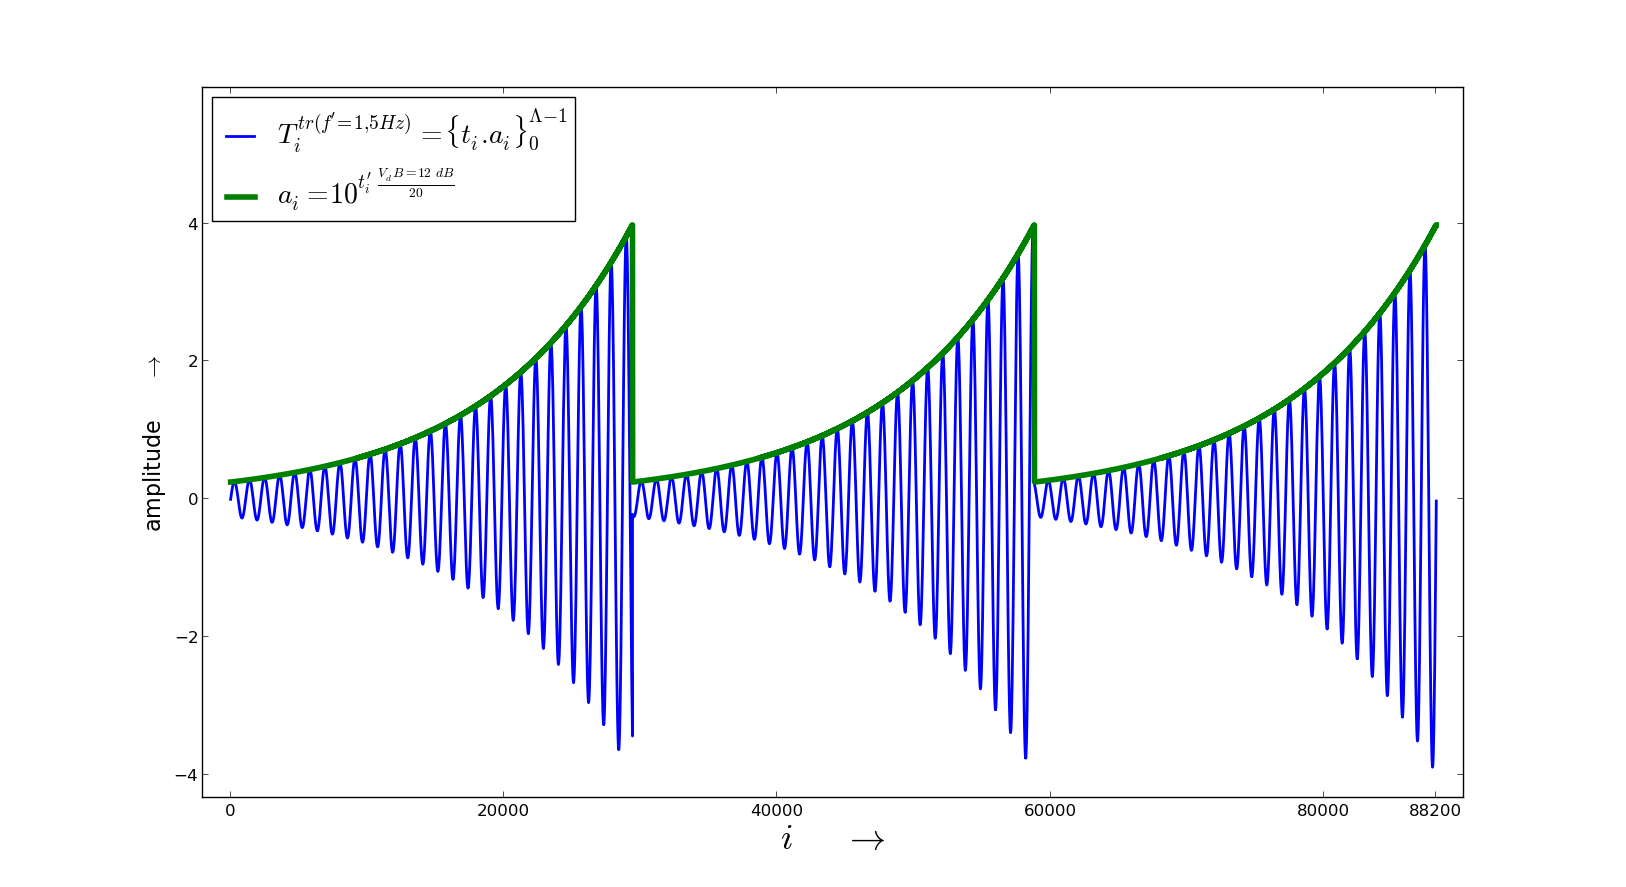
\includegraphics[width=\textwidth]{figuras/tremolo}
    \caption{Tremolo de profundidade $V_{dB}=12dB$ com padrão oscilatório de uma dente de serra em $f'=1.5Hz$ em uma senoide de $f=40Hz$ (considerada taxa de amostragem $f_a=44,1kHz$).}
        \label{fig:tremolo}
\end{figure}

No aumento progressivo de $f'$,
a aproximação do limiar de frequência
para audição do fenômeno sonoro como
altura ($\approx 20Hz$) gera rugosidades para
ambos tremolos e vibratos. Estas rugosidades são muito apreciadas
tanto na tradição erudita quanto na música eletrônica atual, especialmente no \emph{Dubstep}.
A rugosidade também é gerada através de conteúdos espectrais que geram batimentos.\cite{Porres,porres2009} A sequência \emph{Bela Rugosi}
explora este limiar com concomitâncias de tremolos e vibratos na mesma
voz, com intensidades e formas de onda diferentes. Seu código está o Apêndice~\ref{ap:bela} e disponível online como parte da \massa.

Aumentando ainda mais a frequência, estas oscilações
deixam de ser eventos identificáveis. 
Neste caso, as oscilações são
audíveis como altura. Assim, $f'$, $\mu$ e a forma de onda realizam alterações espectrais no som
original $T_i$ de formas diferentes para os tremolos e para os vibratos. São as 
chamadas sínteses AM (\emph{Amplitude Modulation}) e FM (\emph{Frequency Modulation}), respectivamente.
Estas são técnicas conhecidas, com aplicações em sintetizadores
como o \emph{Yamaha DX7}, e com aplicações fora da música, como em telecomunicações para transmissão de informação via ondas eletromagnéticas (ex. rádios AM e FM).

Para fins musicais e em resumo, pode-se entender a síntese FM através do caso entre senoides
e decompor os sinais em seus espectros de Fourier (i.e. senoidais) para casos mais complexos.
Assim, a síntese FM realizada com um 'vibrato' senoidal de frequência $f'$ e profundidade $\mu$ em um som também senoidal $T_i$ de frequência $f$
gera bandas centradas em $f$ e distantes $f'$ entre si:

\begin{equation}\label{eq:fmEsp}
\begin{split}
\{t_i'\} & = \left \{ \cos \left [f . 2 \pi \frac{i}{f_a-1} + \mu . sen \left ( f' . 2 \pi \frac{i}{ f_a -1 } \right ) \right ] \right \} = \\
 & = \left \{ \sum_{k=-\infty}^{+\infty} J_k(\mu) \cos \left [ f . 2 \pi \frac{i}{f_a-1} + k . f' . 2 \pi \frac{i}{f_a-1} \right ]  \right \} = \\
 & = \left \{ \sum_{k=-\infty}^{+\infty} J_k(\mu) \cos \left [ (f+k.f') . 2 \pi \frac{i}{f_a-1} \right ]  \right \}
\end{split}
\end{equation}

onde 
\begin{equation}\label{eq:Bessel}
J_k(\mu) = \frac{2}{\pi} \int_0^{\frac{\pi}{2}}\left [ cos \left (\overline{k}\;\frac{\pi}{2} + \mu . \sin w \right ) . cos \left ( \overline{k}\;\frac{\pi}{2} + k . w \right ) \right ] dw \quad , \quad \overline{k} = k \% 2 \;\;,\;\; k \in \mathbb{N}
\end{equation}
é a função de Bessel~\cite{BesselCCRMA,JOSFM} que na FM especifica a amplitude de cada componente. 

Nestas equações, a variação de frequência introduzida por $\{t_i'\}$ não respeita a progressão geométrica de frequência que acompanha a percepção de altura, mas sim a equação~\ref{freqLinear}. A utilização das equações~\ref{vbrF} para a FM está no Apêndice~\ref{cap:fmam}, onde é calculado o conteúdo espectral da síntese FM obtida com oscilações na escala logarítmica. De fato, o comportamento simples que torna a FM atraente é obtido somente com as variações lineares em~\ref{eq:fmEsp}.

O caso da modulação de amplitude (AM) é mais simples:

\begin{equation}\label{eq:amEsp}
\begin{split}
\{t_i'\}_0^{\Lambda-1} & =\{(1+a_i) . t_i\}_0^{\Lambda-1}= \left \{ \left [ 1+M.\sin \left ( f'.2\pi\frac{i}{f_a -1} \right ) \right] . P .\sin \left ( f.2\pi\frac{i}{f_a -1} \right ) \right \}_0^{\Lambda-1} = \\
                       & =  \left\{P.\sin \left( f.2\pi\frac{i}{f_a -1}  \right ) + \frac{P.M}{2} \left [ \sin \left( (f-f').2\pi\frac{i}{f_a -1}  \right ) + \sin \left( (f+f').2\pi\frac{i}{f_a -1}  \right ) \right ] \right \}_0^{\Lambda-1}
\end{split}
\end{equation}

Ou seja, o som resultante é o original
e a reprodução de seu conteúdo espectral acima e abaixo da frequência
original, distantes $f'$ de $f$. Novamente, isso é obtido com a variação na escala linear de amplitude. No Apêndice~\ref{cap:fmam} está uma exposição do espectro da AM realizada com a oscilação na escala logarítmica de amplitude. Esta também perde o comportamento simples.

A sequência $T_i$ de frequência $f$, chamada portadora, é modulada pela $f'$, chamada moduladora. No jargão de FM e AM, $\mu$ e $\alpha=10^{\frac{V_{dB}}{20}}$ são chamados índices de modulação. Assim, 
para o padrão de vibração da moduladora $\{t_i'\}$ as equações:

\begin{equation}\label{fmGammaAux}
\gamma_i'=\left \lfloor i f' \frac{\widetilde{\Lambda}_M}{f_a} \right \rfloor
\end{equation}

\begin{equation}\label{fmAux}
t_i'=\widetilde{m}_{\gamma_i' \;\% \widetilde{\Lambda}_M}
\end{equation}

Para aplicação da moduladora $\{t_i'\}$ na portadora $\{t_i\}$
por FM:

\begin{equation}\label{fmF}
f_i=f + \mu . t_i'
\end{equation}

\begin{equation}\label{fmGamma}
\Delta_{\gamma_i}=f_i\frac{\widetilde{\Lambda}}{f_a} \quad \Rightarrow \quad \gamma_i = \left \lfloor \sum_{j=0}^{i} f_j \frac{\widetilde{\Lambda}}{f_a} \right \rfloor = \left \lfloor \sum_{j=0}^{i} \frac{\widetilde{\Lambda}}{f_a}(f+\mu . t_j') \right\rfloor
\end{equation}

\begin{equation}\label{fmT}
T_i^{f,\, FM(f',\,\mu)}=\left\{ t_i^{f,\,FM(f',\,\mu)} \right\}_0^{\Lambda-1}=\left\{\,\widetilde{l}_{\gamma_i \%\; \widetilde{\Lambda} } \,\right\}_0^{\Lambda-1}
\end{equation}

Onde $\widetilde{l}$ é um período da forma de onda de comprimento $\widetilde{\Lambda}$ da portadora.

Para realizar a AM, basta modular $\{t_i\}$ com $\{t_i'\}$ através das equações:

\begin{equation}\label{amA}
a_i=1 + \alpha . t_i'
\end{equation}

\begin{equation}\label{amT}
T_i^{f,\,AM(f',\,\alpha)}=\left\{ t_i^{f,\,AM(f',\,\alpha)} \right\}_0^{\Lambda-1}=\{ t_i . a_i \}_0^{\Lambda-1}=\{t_i . (1 + \alpha . t_i')    \}_0^{\Lambda-1}
\end{equation}



\subsection{Usos musicais}\label{subsec:mus2}
A este ponto as possibilidades musicais explodiram. As
características de altura (dada pela frequência),
timbre (dado pela forma de onda e filtragens),
volume (dado pela intensidade) e duração (dada pelo número de amostras)
podem ser consideradas
de forma absoluta ou tratadas ao longo de sua duração,
com a única exceção da duração em si.

Desta forma, os usos musicais aqui dispostos são uma coleção de possibilidades
com o objetivo de exemplificar manipulações sonoras que resultem algo
musical, por razões variadas e aprofundadas na próxima seção.

Uma primeira possibilidade interessante é usar vínculos
entre os parâmetros do tremolo e do vibrato e algum parâmetro da nota básica,
como a frequência. Assim, pode-se estabelecer que
a frequência do vibrato é diretamente proporcional à altura, e a profundidade do tremolo é inversamente proporcional
à altura.
Desta forma, com as equações \ref{vbrGamma}, \ref{vbrF} e \ref{trA}
pode-se escrever:

\begin{equation}\label{eq:vinculos}
\begin{split}
f^{vbr} = f^{tr} & = func_a(f) \\
\nu & = func_b(f) \\
V_{dB} & = func_c(f)
\end{split}
\end{equation}

Com $f^{vbr}$ e $f^{tr}$ como $f'$ nas equações de referência, ou seja, a frequência
de oscilação do vibrato e do tremolo da equação~\ref{vbrGamma}. Já $\nu$ e $V_{dB}$ são as profundidades
do vibrato e do tremolo, respectivamente. As funções $func_a$,
$func_b$ e $func_c$ são arbitrárias e dependentes das intenções musicais. A montagem 
\emph{Tremolos, vibratos e a frequência} explora
recursos como este e variações da forma de onda da oscilação com vínculos, de modo a formar um \emph{idioma musical}\footnote{Veja na próxima seção.}. Seu código está no Apêndice~\ref{ap:tremolos} e também disponível online como parte da caixa de ferramentas \massa.


Com relação à convolução, pode-se estabelecer uma duração como pulso musical - a exemplo de um pulso BPM - 
e distribuir impulsos no decorrer deste pulso, de forma a estabelecer métricas e ritmos\footnote{Lembrando
que a convolução com o impulso resulta no som deslocado ao instante de ocorrência do impulso.}.
Por exemplo, 2 impulsos igualmente espaçados fazem uma
divisão binária básica do pulso. Dois sinais, um com 2 pulsos e outro com 3 pulsos,
ambos com os impulsos igualmente espaçados na duração do pulso, resultam na manutenção
do pulso, com uma marcação rítmica usada tanto em divisões binárias quanto ternárias em diversos
estilos de música étnica e tradicional.\cite{Gramani} 
Os próprios valores absolutos destes impulsos resultam em proporções entre as amplitudes dos sinais
convoluídos.
Este recurso da métrica
estabelecida pela convolução com impulsos é explorado na montagem \emph{Trenzinho de caipiras impulsivos}. Os recursos explorados incluem a criação de amálgamas sonoros provenientes da síntese granular e esta montagem é já uma ponte para a próxima seção. Veja especialmente a figura~\ref{fig:pulsoSubAgl}. O código da peça está na seção~\ref{ap:trenzinho} e disponível como parte da toolbox \massa.

Com os filtros as possibilidades explodem ainda mais vertiginosamente. Pode-se convoluir um sinal para reverberá-lo, para
remover algum ruído, para gerar distorções ou para tratamento com intuito estético mesmo. Por exemplo,
a aplicação de um filtro passa banda em que deixa passar somente entre $1kHz$ e $3kHz$, resulta em sons
que parecem de telefone ou de televisão antiga. Ao remover com alguma precisão somente
a frequência de oscilação da rede elétrica (usualmente $50Hz$ ou $60Hz$) e harmônicas, pode-se remover
ruídos introduzidos por equipamentos de áudio.
Um uso mais incrementado
e propriamente musical é realizar filtragens em bandas específicas e usar estas bandas
pré-estabelecidas como um parâmetro adicional das notas.

Inspirado em nos instrumentos tradicionais, pode-se aplicar uma a filtragem dependente do tempo~\cite{Roederer}.
Cascatas
destes filtros podem realizar filtragens complexas e mais precisas. A montagem \emph{Ruidosa faixa} explora
este recursos, realizando filtragens em ruídos diversos e síntese de ruídos diversos. O código da peça está no Apêndice~\ref{ap:ruidosa} e disponível online como parte da \massa.

Estes recursos todos utilizados em conjunto podem incidir na realização de um efeito chamado \emph{chorus}. A
exemplo do que ocorre com um coro de cantores, neste efeito o som é realizado com diversas pequenas modificações,
potencialmente aleatórias, em paramêtros como frequência central, presença (ou ausência) de vibrato
e tremolo e suas características, equalizações, volume etc. Para o resultado final, estas versões do som
inicial são então mixadas (ver equação \ref{eq:mixagem}). A peça \emph{Chorus infantil} realiza chorus de formas
diferentes em sons diferentes e seu código está no Apêndice~\ref{ap:chorus}. A \emph{toolbox} \massa\ disponibiliza online este \emph{script}.

A variação de volume no decorrer de um som é crucial para nossa percepção de timbre. A envoltória de volume chamada ADSR (sigla de \emph{Atack-Decay-Sustain-Release}) possui numerosas implementações em sintetizadores em hardware e software. Uma implementação pioneira pode ser encontrada no Hammond Novachord de 1938 e algumas variantes são citadas logo abaixo.\cite{ADSR}

A envoltória ADSR escolástica é caracterizada por 4 parâmetros: duração do ataque (tempo que o som demora para atingir seu volume máximo), duração do decaimento (segue ao ataque imediatamente), nível de volume de sustentação (em que o volume fica estável após o decaimento) e duração de soltura (após a sustentação, nesta duração o volume decai a zero).
Note que o tempo de sustentação não é especificado, pois é resultante da duração em si menos os tempos de ataque, decaimento e soltura.

A aplicação da envoltória ADSR com durações $\Delta_A$, $\Delta_D$ e $\Delta_R$, duração total $\Delta$ e nível de sustentação $a_S$, dado
como fração da amplitude máxima, em uma sequência sonora $t_i$ qualquer, pode ser feita da seguinte forma:

\begin{equation}\label{eq:adsr}
\begin{split}
\{a_i\}_0^{\Lambda_A-1} & = \left\{\xi\left(\frac{1}{\xi}\right)^{\frac{i}{\Lambda_A-1}}\right\}_0^{\Lambda_A-1} \;\;\quad\quad\quad \text{ou} \;\;\quad \left\{\frac{i}{\Lambda_A-1}\right\}_0^{\Lambda_A}\\
\{a_i\}_{\Lambda_A}^{\Lambda_A+\Lambda_D-1} & =\left\{a_S^{\frac{i-\Lambda_A}{\Lambda_D-1}}  \right\}_{\Lambda_A}^{\Lambda_A+\Lambda_D-1} \;\;\quad \quad\quad \text{ou} \quad\;\; \left\{1-(1-a_S)\frac{i-\Lambda_A}{\Lambda_D-1}\right\}_{\Lambda_A}^{\Lambda_A+\Lambda_D-1}\\
\{ a_i \}_{\Lambda_A+\Lambda_D}^{\Lambda-\Lambda_R-1} & =\left\{ a_S \right\}_{\Lambda_A+\Lambda_D}^{\Lambda-\Lambda_R-1} \\
\{ a_i \}_{\Lambda-\Lambda_R}^{\Lambda-1} & =\left\{ a_S\left(\frac{\xi}{a_S} \right)^{\frac{i-(\Lambda-\Lambda_R)}{\Lambda_R-1}} \right\}_{\Lambda-\Lambda_R}^{\Lambda-1} \quad\;\; \text{ou} \quad\;\; \left\{ a_S - a_S\frac{i+\Lambda_R-\Lambda}{\Lambda_R-1}\right\}_{\Lambda-\Lambda_R}^{\Lambda-1} 
\end{split}
\end{equation}

Com $\Lambda_X=\lfloor \Delta . f_a \rfloor\;\;\forall\;\; X \; \in (A,D,R,\;)$ e $\xi$ um valor pequeno que torne o \emph{fade in} e o \emph{fade out} satisfatórios, e.g. $\xi=10^{\frac{-80}{20}}=10^{-4}\;$ ou $\;\xi=10^{\frac{-40}{20}}=10^{-2}$. Quanto menor for $\xi$ mais lento é o \emph{fade}, a exemplo de $\alpha$ da figura~\ref{fig:transicao}. Já os termos do lado direito de~\ref{eq:adsr} podem realizar as entrada e saída do som a partir da intensidade zero, por serem lineares. 
Esquematicamente, a figura~\ref{fig:adsr} mostra esta envoltória ADSR, 
uma implementação clássica que comporta variações diversas. Por exemplo,
entre o ataque e o decaimento, pode-se adicionar uma partição adicional em que a amplitude
máxima perdura. Outro exemplo comum é o uso de traçados mais elaborados para o
ataque ou para o decaimento. A montagem musical \emph{ADa e SaRa}, disponível no Apêndice~\ref{ap:ada}
e na \massa, explora diversas destas configurações da envoltória ADSR


\begin{equation}\label{eq:adsrApl}
\left\{t_i^{ADSR}\right\}_0^{\Lambda-1} =\{t_i . a_i\}_0^{\Lambda-1}
\end{equation}

\begin{figure}[htpq!]
    \centering
        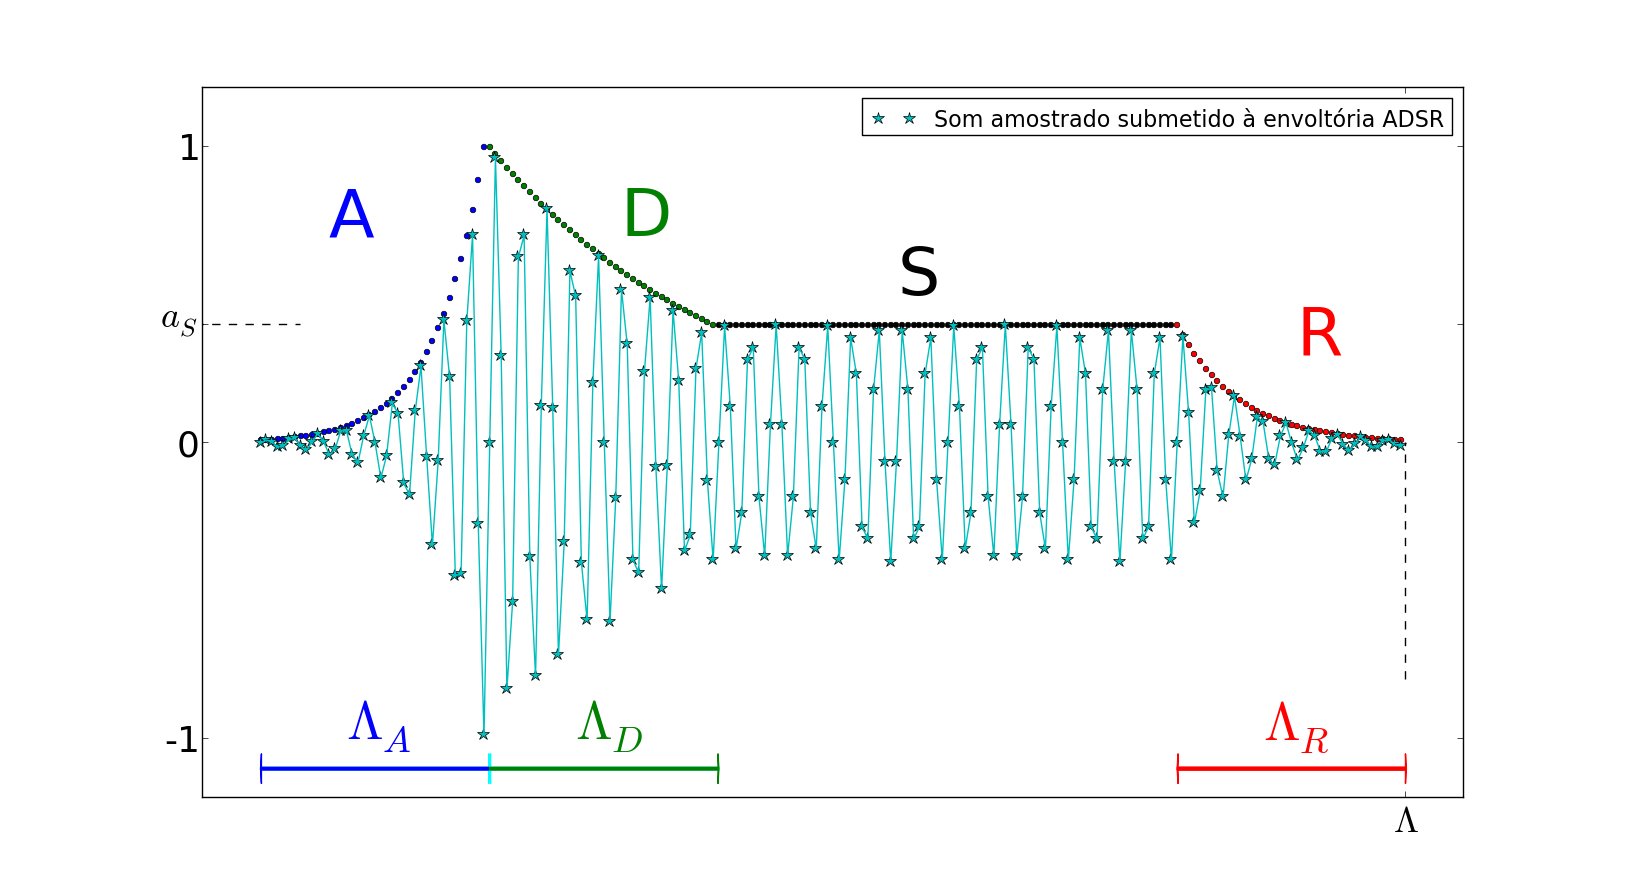
\includegraphics[width=\textwidth]{figuras/adsr}
    \caption{Envoltória ADSR (\emph{Attack, Decay, Sustain, Release}) e uma sequência sonora arbitrária submetida à envoltória. A variação linear de amplitude está acima. Abaixo a variação de amplitude é exponencial.}
\end{figure}
        \label{fig:adsr}



\clearpage
\section{Organização de notas em música}\label{notasMusica}
Seja $ S_j=\left\{  s_j=T_i^j=\{t_i^j\}_{i=0}^{\Lambda_j-1} \right\}_{j=0}^{H-1} $ uma sequência $S_j$ de $H$ eventos
musicais $s_j$. Seja $S_j$ chamada uma 'estrutura musical' composta de eventos $s_j$ que são também estruturas musicais,
p.ex. notas.
Esta seção é dedicada às técnicas que tornam $S_j$ interessante e agradável na audição.

Os elementos de $S_j$ podem ser sobrepostos por mixagem, como na equação~\ref{eq:mixagem} e figura~\ref{fig:mixagem}, formando intervalos e acordes. Este é o 'pensamento vertical' da música. A concatenação de $S_j$, como na equação~\ref{eq:concatenacao} e na figura~\ref{fig:concatenacao}, forma sequências melódicas e ritmos, associados ao 'pensamento horizontal' na música. A frequência fundamental $f$ e o momento de início (ataque) são, em geral, as características mais importantes dos elementos de $S_j$. Estas viabilizam músicas de alturas (harmonia e melodia) e a presença da métrica temporal e ritmos, respectivamente.



\subsection{Afinação}
O dobro da frequência é uma oitava ascendente ($f=2f_0$).
A divisão da oitava em doze notas é o cânone da música ocidental clássica,
além de usos cerimoniais/religiosos e étnicos observados fora da tradição ocidental.\cite{Wisnick}
Doze semitons equidistantes para o ouvido formam uma oitava,
portanto, se $f=2^{\frac{1}{12}}f_0$, há um semitom entre $f_0$
e $f$.
O fator $\varepsilon=2^{\frac{1}{12}}$, um semitom, forma uma grade de notas
no espectro audível. Fixada uma frequência $f$, as frequências fundamentais possíveis
estão separadas por intervalos múltiplos de $\varepsilon$.
Esta precisão absoluta é característica de implementações
computacionais, pois os intrumentos reais possuem desvios destas frequências para melhor compatibilizar os harmônicos
de suas notas. Além disso, o fator fixo $\varepsilon=2^{\frac{1}{12}}$ caracteriza
a afinação de temperamento por igual. Há afinações com intervalos propostos como razões de inteiros de baixa ordem, com
fundamentação em leis físicas, e foram propostas antes do advento do temperamento por igual.\cite{Roederer}

Duas afinações emblemáticas são:
\begin{itemize}
    \item A {\bf intonação justa} consiste em notas da escala diatônica descritas como razão de inteiros de pequena ordem como apontados pela série harmônica. As razões básicas estão contidas no modo jônico (dó a dó nas teclas brancas do piano, veja abaixo na subseção~\ref{subsec:escalas}): 1, 9/8, 5/4, 4/3, 3/2, 5/3, 15/8, 2/1. Os intervalos são considerados com relação às notas das escala e são usados o semitom 16/15, o 'tom menor' 10/9 e o 'tom maior' 9/8. Há diferentes formas de realizar uma divisão de 12 notas.
    \item A {\bf afinação pitagórica} baseia-se no intervalo 3/2 (quinta justa). O modo jônico fica: 1, 9/8, 81/64, 4/3, 3/2, 27/16, 243/128, 2/1. Os intervalos são também considerados com relação às notas da escala. Além dos intervalos do modo, são usados a segunda menor 256/243, a terça menor 32/27, a quarta aumentada 729/512, a quinta diminuta 1024/729, a sexta menor 128/81 e a sétima menor 16/9. 
\end{itemize}

Para a realização de microtonalidade\footnote{O uso de
intervalos menores que o semitom é chamado microtonalidade e tem usos
ornamentais e estruturantes da música. A
divisão da oitava em $12$ notas possui fundamentos físicos mas
não deixa de ser uma \emph{convenção}
adotada inclusive pela música erudita clássica de origem européia. Outras afinações
são incidentes. Para citar somente um exemplo, a
música tradicional tailandesa utiliza uma divisão da oitava em sete notas igualmente
espaçadas ($\varepsilon=2^{\frac{1}{7}}$),
resultando em intervalos que pouco se assemelham aos intervalos na
divisão de doze notas.\cite{Wisnick}},
pode-se usar reais não inteiros
para a sequência de alturas, ou modificar o fator $\varepsilon=2^{\frac{1}{12}}$
e continuar usando inteiros. Por exemplo, uma afinação
bastante próxima da série harmônica em si
é proposta na forma da divisão da oitava em $53$ notas:
$\varepsilon_2=2^{\frac{1}{53}}$.\cite{microtonalidade}
As notas nesta divisão da oitava em $53$ notas se relacionam por inteiros
com $\varepsilon_2$.
Note que se $S_i$ é uma sequência de alturas relacionadas por $\varepsilon_1$,
um mapeamento para notas em $\varepsilon_2$
constitui uma nova sequência $S_i'$ com $s_i'=s_i \frac{\varepsilon_1}{\varepsilon_2}$. A montagem musical \emph{Micro tom} explora recursos microtonais e seu código está no Apêndice~\ref{ap:micro}, assim como na \massa\ online.



\subsection{Intervalos}\label{subsec:intervalos}
Em proporções de $\varepsilon=2^{\frac{1}{12}}$ entre as frequências das notas (i.e. um semitom), os intervalos do sistema de 12 notas são representados por inteiros. A tabela~\ref{eq:intervalos} resume as características de cada intervalo: sua nomenclatura tradicional, características de consonância e dissonância e número de semitons de cada um.

\begin{table}[htpq!]
\centering
\caption{Intervalos musicais, suas notações tradicionais, classificações básicas de dissonância e número de semitons.
As consonâncias perfeitas são os uníssonos, as quintas e as oitavas justas (J). As consonâncias imperfeitas são
as terças e as sextas maiores (M) e menores (m). As dissonâncias fortes são as segundas menores e sétimas maiores. As dissonâncias
brandas são as segundas maiores e as sétimas menores. O primeiro caso especial consite na quarta justa, que é consonante perfeita
se considerada uma inversão da quinta justa, caso contrário pode ser considerada uma dissonância ou uma consonância imperfeita. O segundo caso especial é o trítono (4aum, 5dim, tri). Este é consonante em algumas culturas, já para a música tonal, o trítono indica dominante e busca fundamentalmente sua resolução em uma terça ou sexta e, por esta instabilidade, é considerado intervalo dissonante.}
\begin{tabular}{| c | c | c | }\hline
    \multicolumn{3}{|c|}{\bf consonâncias}  \\\hline
   & notação tradicional & número de semitons \\
   perfeitas: & 1J, 5J, 8J & 0, 7, 12 \\
 imperfeitas: & 3m, 3M, 6m, 6M & 3, 4, 8, 9 \\\hline\hline
    \multicolumn{3}{|c|}{\bf dissonâncias} \\\hline
 & notação tradicional & número de semitons \\
 fortes: & 2m, 7M & 1, 11 \\
 brandas: & 2M, 7m & 2, 10 \\\hline\hline
    \multicolumn{3}{|c|}{\bf casos especiais} \\\hline
 & notação tradicional & número de semitons \\
 consonante ou dissonante: & 4J & 5 \\
 dissonante na tradição ocidental: & trítono, 4aum, 5dim & 6 \\\hline
\end{tabular}\label{eq:intervalos}
\end{table}


A nomenclatura, com base em imposições e conveniências do sistema tonal, e de aspectos práticos da manipulação de notas, pode ser especificada assim:\cite{Roederer,Wisnick}
\begin{itemize}
        \item Intervalos por número de grados entre as notas: primeira (uníssono), segunda, terça, quarta, quinta, sexta, sétima, oitava. Nona, décima, décima primeira, etc, são os intervalos compostos, de uma ou mais oitavas + um intervalo dentro da oitava, que caracteriza o intervalo composto. São representados pelos dígitos numéricos: 1, 3, 5 é um uníssono, uma terça, e uma quinta.
        \item Qualidades de cada intervalo: as consonâncias perfeitas - i.e. uníssono, quarta, quinta e oitava - são 'justas'. As consonâncias imperfeitas - i.e. terças e sextas - e as dissonâncias - i.e. segundas e sétimas - podem ser maiores ou menores. Excessão para o trítono.
        \item A quarta justa é tida como consonante perfeita ou dissonante de acordo com o contexto e arcabouço teórico. Como regra geral, pode ser considerada consonante salvo casos em que é usada de passagem para uma quinta ou terça como resolução.
        \item O trítono é dissonante na música ocidental por caracterizar a "dominante" no sistema tonal (veja abaixo na subseção~\ref{subsec:harmonia}) e representar instabilidade. Algumas culturas entoam o intervalo como consonante.
        \item Um intervalo maior, descrescido de um semitom, resulta em um intervalo menor. Um intervalo menor, acrescido de um semitom, resulta em um intervalo maior.
        \item Um intervalo justo (uníssono, quarta justa, quinta justa, oitava justa), ou um intervalo maior (segunda maior 2M, terça maior 3M, sexta maior 6M ou sétima maior 7M), acrescido de um semitom, resulta em um intervalo aumentado (p.ex. terça aumentada 3aum com cinco semitons). A quarta aumentada é também chamada de trítono (4aum ~ tri).
        \item Um intervalo justo, ou um intervalo menor (segunda menor 2m, terça menor 3m, sexta menor 6m ou sétima menor 7m), decrescido de um semitom, resulta em um intervalo diminuto. A quinta diminuta é também chamda de trítono (5dim ~ tri).
        \item Um intervalo aumentado, acrescido de um semitom, resulta em um intervalo 'mais que aumentado' e um intervalo diminuto, descrescido de um semitom, resulta em um intervalo 'mais que diminuto'.
        \item Caso as notas soem simultaneamente, o intervalo é harmônico.
        \item Caso as notas soem em sequência no tempo, o intervalo é melódico. A ordem das notas, primeiro a nota mais grave ou a mais aguda, resulta em um intervalo ascendente ou descendente, respectivamente. 
        \item Passando a nota mais grave para a oitava acima, ou a nota mais aguda uma oitava para baixo, o intervalo é invertido. Um intervalo, somado à sua inversão, resulta 9 (7m inverte para 2M: $7m+2M=9-$). Um intervalo maior invertido resulta em um intervalo menor e vice-versa. Um intervalo aumentado invertido resulta diminuto e vice-versa, assim como o mais que aumentado resulta em mais que diminuto e vice-versa. Um intervalo justo invertido resulta igualmente justo.
        \item Um intervalo maior que a oitava é dito 'intervalo composto' e é classificado como o intervalo entre as mesmas notas, mas na mesma oitava. São também especificados por 7 acrescido deste intervalo: 11J é uma oitava mais uma quarta (7+4J==11J), 9M é uma oitava mais uma segunda (7+2M=9M).
\end{itemize}

Os intervalos aumentados/diminutos e mais que aumentados/diminutos são consequências do sistema tonal. Os graus da escala (veja abaixo na subseção~\ref{subsec:escalas}) são realmente notas diferentes, com funções e usos específicos. Assim, em uma escala de dó bemol maior, a tônica - primeiro grau - é dó bemol, não si, e a sensível - sétimo grau - é si bemol, não lá sustenido ou dó duplo bemol. De forma semelhante, o segundo grau de uma escala pode estar a um semitom do primeiro grau, assim como a sensível (sétimo grau a um semitom ascendente do primeiro), momento no qual há uma terça diminuta entre os dois semitons do sétimo e segundo grau da escala pois o primeiro grau está entre os dois graus próximos a ele: segundo e sensível.\cite{Lacerda}

Esta descrição resume a teoria tradicional dos intervalos musicais.\cite{Lacerda} A montagem \emph{Intervalos entre alturas} explora estes intervalos de formas isoladas e diversas. O código está no Apêndice~\ref{ap:intervalos} e disponível online com a \emph{toolbox} \massa.\cite{MASSA}


\subsection{Escalas}\label{subsec:escalas}
Uma escala é um conjunto ordenado de alturas. Usualmente, as escalas se repetem
a cada oitava. A sequências ascendente com todas as notas da divisão da oitava em 12 intervalos iguais
separados pela razão $\varepsilon=2^{\frac{1}{12}}$ é a escala cromática de temperamento igual. Há 5 divisões perfeitamente simétricas da oitava dentro da escala cromática. Estas divisões são consideradas
escalas pelos usos fáceis e peculiares que disso provém. Como inteiros aos quais $\varepsilon=2^{\frac{1}{12}}$ é elevado
para multiplicar $f_0$, as escalas são:

\begin{equation}\label{escSim}
\begin{split}
\text{cromática} & = E_i^c = \{e_i^c\}_0^{11} =  \{0,1,2,3,4,5,6,7,8,9,10,11\} = \{i\}_0^{11}\\
\text{tons inteiros} & = E_i^t = \{e_i^t\}_0^{5} = \{0,2,4,6,8,10\} = \{2.i\}_0^{5} \\
\text{terças menores} & = E_i^{tm} = \{e_i^{tm}\}_0^{3} = \{0,3,6,9\} = \{3.i\}_0^3 \\
\text{terças maiores} & = E_i^{tM} = \{e_i^{tM}\}_0^{2} = \{0,4,8\} = \{4.i\}_0^2\\
\text{trítonos} & = E_i^{tt} = \{e_i^{tt}\}_0^{1} = \{ 0, 6 \} = \{6.i\}_0^1
\end{split}
\end{equation}

Assim, a terceira nota da escala em tons inteiros com $f_0=200Hz$
é $f_3=\varepsilon^{e_3^t} . f_0 = 2^{\frac{6}{12}} . 200 \approxeq 282.843 Hz$. Estas
'escalas' ou padrões, geram estruturas estáveis pelas simetrias internas, e podem ser
repetidas de forma eficiente e sustentada. Abaixo, na seção~\ref{estCic}. A montagem \emph{Cristais} expõe cada uma destas escalas tanto melódica quanto harmonicamente e seu código está no Apêndice~\ref{ap:cristais}. Como parte da \massa, este código é disponibilizado online.

As escalas diatônicas:

\begin{equation}\label{eq:escalas}
\begin{split}
\text{menor natural} = \text{modo eólico} & = E_i^m = \{e_i^m\}_0^6 = \{0,2,3,5,7,8,10\} \\
\text{modo lócrio} & = E_i^{mlo} = \{e_i^{mlo}\}_0^6 = \{0,1,3,5,6,8,10\} \\ 
\text{maior}  = \text{modo jônico} & = E_i^M = \{e_i^M\}_0^6 = \{0,2,4,5,7,9,11\} \\
\text{modo dórico} & = E_i^{md} = \{e_i^{md}\}_0^6 = \{0,2,3,5,7,9,10\} \\
\text{modo frígio} & = E_i^{mf} = \{e_i^{mf}\}_0^6 = \{0,1,3,5,7,8,10\} \\
\text{modo lídio} & = E_i^{ml}=\{e_i^{ml}\}_0^6 = \{0,2,4,6,7,9,11\} \\
\text{modo mixolídio} & = E_i^{mmi} = \{e_i^{mmi}\}_0^6 = \{0,2,4,5,7,9,10\}
\end{split}
\end{equation}

possuem apenas intervalos maiores, menores e justos. Única exceção para o trítono, que se apresenta como quarta aumenta ou quinta diminuta.

Todas as escalas diatônicas
seguem o padrão de intervalos sucessivos
tom, tom, semitom, tom, tom, tom, semitom, e
pode-se escrever:
\begin{equation}\label{eq:relacaoDia}
\begin{split}
\{d_i\} & =\{2,2,1,2,2,2,1\} \\
e_0 & =0 \\
e_i & =d_{(i+\kappa)\%7}+e_{i-1} \quad para \;\;  i > 0
\end{split}
\end{equation}

Com $\kappa \in \mathbb{N}$. Para cada
modo, há um único valor de $\kappa \in [0,6]$.
Por exemplo, uma breve
inspeção revela que $e_i^{ml}=d_{(i+2)\%7}+e_{i-1}^{ml}$. Portanto, $\kappa=2$
para o modo lídio. 

A escala menor possui duas formas adicionais, melódica e harmônica:

\begin{equation}\label{eq:escalasMenores}
\begin{split}
\text{menor natural (igual acima)} & = E_i^m = \{e_i^m\}_0^6 = \{0,2,3,5,7,8,10\} \\
\text{menor harmônica} & = E_i^{mh} = \{e_i^{mh}\}_0^6 = \{0,2,3,5,7,8,11\} \\
\text{menor melódica} & = E_i^{mm} = \{e_i^{mm}\}_0^{14} = \{0,2,3,5,7,9,11,12,10,8,7,5,3,2,0\} \\
\end{split}
\end{equation}

O traçado ascendente e descendente da escala menor melódica é necessário para a presença da sensível (sétimo e último grau separado por um semitom da oitava e realça a polarização na tônica) no trajeto ascendente, o que não é necessário quando descende, retomando a forma natural. Já a escala harmônica apresenta a sensível, mas não evita o intervalo de segunda aumentada entre o sexto e sétimo graus, pois não precisa contemplar trajetória melódica, apenas apresentar a sensível tão cara ao sistema tonal (a sensível tende à tônica, afirmando-a).\cite{Harmonia}
Outras escalas podem ser representadas da mesma forma, como as pentatônicas e os modos de transposição limitados de Messiaen.\cite{Messiaen}

\subsection{Acordes}\label{subsec:acordes}
A ocorrência simultânea de notas é observada através dos acordes. Destes, a base na música tonal são as tríades. Estas constituem-se de duas terças sucessivas, em 3 notas: fundamental, terça e quinta. Um acorde invertido é aquele que apresenta no grave outra nota que não a fundamental. A posição fechada é aquela em que não cabe nota alguma do acorde entre quaisquer duas notas consecutivas.\cite{Lacerda}
As tríades, sem inversão, na forma fechada e com a fundamental em $0$, são:

\begin{equation}\label{triades}
\begin{split}
\text{tríade maior} = A_i^M= \{a_i^M\}_0^2=\{0,4,7\} \\ 
\text{tríade menor} = A_i^m = \{a_i^m\}_0^2=\{0,3,7\} \\
\text{tríade diminuta} = A_i^d = \{a_i^d\}_0^2=\{0,3,6\} \\
\text{tríade aumentada} = A_i^a = \{a_i^a\}_0^2=\{0,4,8\}
\end{split}
\end{equation}

Para considerar outra terça sobreposta à quinta, basta acrescentar $10$ ao final para a tétrade
com sétima menor ou $11$ para a tétrade com sétima maior. As inversões e posições abertas
podem ser obtidas com a adição seletiva de $12$ às componentes.

Acordes triádicos incompletos, com notas adicionais (acordes 'sujos'), e não triádicos são comuns.
Orientações gerais são:
\begin{itemize}
    \item Uma quinta constitui uma fundamental confirmada pelo intervalo.
    \item A terça maior ou menor aponta a qualidade maior ou menor do acorde.
    \item Todo trítono, especialmente se formado entre uma terça maior e uma sétima menor, tende a resolver em uma terça ou uma sexta.
    \item Na repetição, a ordem de preferência é: a fundamental, a quinta, a terça e a sétima.
    \item Pode-se formar acordes com notas diferentes das triádicas, especialmente se dentro de alguma lógica recorrente ou encadeamento musical que justifique as notas diferentes.
    \item Acordes formados por sucessões de intervalos diferentes da terças, como as quartas ou as segundas, são recorrentes dentre composições de tonalismo avançado ou experimentais.
    \item A repetição de sucessões de acordes (ou suas características) fixa uma trajetória pela recorrência e permite a introdução de formações exóticas sem que haja incoerência.
\end{itemize}


\subsection{Harmonia}\label{subsec:harmonia}

Omitir os encadeamentos básicos do sistema tonal é a chave para a obtenção de 
harmonias modal e atonal. No caso desta ausência de estruturas tonais mínimas,
se as notas coincidirem com alguma escala diatônica (veja as equações ~\ref{eq:escalas})
ou forem em número pequeno, pode-se dizer que a
harmonia é modal. Caso encadeamentos tonais básicos estejam ausentes, a notas não coincidam
com alguma das escalas diatônicas e forem diversos e dissonantes o suficiente para evitar redução por
polarizações, a harmonia é atonal.
Nesta classificação, a harmonia modal não é tonal e não é atonal.
A harmonia modal está reduzida à incidência de notas dentro de escalas diatônicas.
Pode-se perceber, pelo conceito, que a harmonia atonal é difícil de ser realizada.\cite{harmEXT}

De fato, as técnicas de música atonal
visam estruturas que evitam o vínculo da audição a modos e relações tonais. A
dificuldade é tamanha que o dodecafonismo surgiu. A proposta do dodecafonismo é
usar um conjunto de notas, idealmente usa-se as 12 notas, e executar uma a uma destas notas
na mesma ordem. Neste contexto, a tônica fica difícil de se estabelecer. Mesmo assim, a audição ocidental
procura traços tonais nas música e facilmente os encontra por caminhos inesperados e por vezes tortuosos.
A utilização de
intervalos dissonantes, especialmente trítonos sem resoluções, nonas, segundas e sétimas, reforça
a ausência de tonalidade. Neste contexto, para criação da peça, pode-se:
\begin{itemize}
    \item Repetir notas, como artifício de sua incidência anterior, não adiciona informação relevante.
    \item Tocar notas adjacentes ao mesmo tempo, em bloco.
    \item As durações podem ser livres, desde que respeitada ordem de aparição das notas.
    \item Para variação, além dos recursos de ampliação, transposição e translação, são usados o inverso, o retrógrado e o retrógrado do inverso. Veja nas subseções~\ref{subsec:motivos} e~\ref{subsec:usosmusicais3} para maiores detalhes.
    \item Variações de intrumentação, articulação, espacialização e outras possibilidades de apresentação da estrutura de notas.
\end{itemize}

A harmonia atonal pode ser observada, de forma paradigmática, dentro destas condições.
Vale apontar que boa parte do que escreveram os compositores
emblemáticos para o dodecafonismo, como Alban Berg e o próprio Schoenberg, consiste
aplicações parciais e livres destas técnicas. Várias peças fazem até mesmo pontes
propositais entre técnicas tonais e atonais.

No século XX, músicas rítmicas
e com ênfase em sonoridades/timbres ampliaram 
as concepções de tonalidade e harmonia. Ainda assim, a harmonia tonal tem forte presença
nas vertentes artísticas e comerciais. O próprio dodecafonismo considera-se de natureza
tonal pois consiste na negação de suas características de polarização.

Na música tonal ou modal, acordes, como os listados nas equações~\ref{triades}, constituídos com a fundamental em cada
grau de escalas especificadas nas equações~\ref{eq:escalas}, formam os pilares do campo harmônico.
A observação de progressões incidentes de acordes e regras para encadeamentos é o objeto de estudo da harmonia musical.
Mesmo uma melodia monofônica gera campos harmônicos e pode-se observar acordes sugeridos por cada passagem.



Na 'harmonia tonal tradicional',
a escala pode ter como tônica (primeiro grau da escala) qualquer nota e pode ser maior (com as mesmas notas do modo jônico) ou menor (as notas do eólico constituem a escala "menor natural" e esta possui versões harmônica e melódica, veja a equação~\ref{eq:escalasMenores}. A escala escolhida é
base para tríades, cada uma com a fundamental em um grau 
da escala: $\hat{1},\hat{2},\hat{3},\hat{4},\hat{5},\hat{6},\hat{7}$. Para a formação do acorde, são consideradas a terceira nota e a quinta nota acima da fundamental, considerando a própria nota como a primeira e utilizando as notas da escala.
Pode-se anotar $\hat{1},\hat{3},\hat{5}$ para o acorde do primeiro grau, formado pelo primeiro grau da escala e central para uma música tonal. Secundários são os acordes do quinto grau $\hat{5},\hat{7},\hat{2}$ ($\hat{7}$ sustenido no caso da escala menor) e do quarto grau $\hat{4},\hat{6},\hat{1}$. Depois são considerados os outros graus. A harmonia tradicional consiste em convenções e técnicas estilísticas de encadeamento destes acordes, formados em cada grau da escala.\cite{Harmonia}

A 'harmonia funcional' atribui funções a estes três acordes centrais e busca compreender seus usos através destas funções. O acorde formado sobre o primeiro grau é o acorde de tônica (T ou t se tônica maior ou menor) e tem a função de manter um centro, um "chão" na música. O acorde formado sobre o quinto grau é a dominante (D, a dominante é sempre maior) e tem a função de tender à tônica, direcionar a música para ela. A tríade formada sobre o quarto grau é a subdominante (S ou s se subdominante maior ou menor) e tem a função de distanciar a música da tônica. O sistema se baseia em afirmar a tônica através de encadeamentos tônica-dominante-tônica expandidos com outros acordes das formas mais diversas.

A estes três acordes, são associadas as outras tríades. Na escala maior, a associada relativa (tônica relativa Tr, subdominante relativa Sr e dominante relativa Dr) é a tríade formada uma terça abaixo e a associada anti-relativa (tônica anti-relativa Ta, subdominante anti-relativa Sa e a dominante anti-relativa Da) é a tríade formada na terça acima. Na escala menor ocorre o mesmo, mas a tríade a uma terça abaixo é chamada anti-relativa (tA, sA) e a tríade a uma terça acima é chamada de relativa (tR, sR). As exatas funções e efeitos musicais destes acordes é motivo de bastante controvérsia. A tabela~\ref{tab:harmonia} mostra a relação entre as tríades formadas em cada grau da escala.

\begin{table}[htpq!]
\centering
\caption{Resumo das funções harmônicas tonais para a escala maior. A tônica é o centro da música, a dominante tende à tônica e a subdominante se distancia da tônica. Os três acordes podem, a princípio, serem substituídos livremente pelas respectivas relativas ou anti-relativas.}
\begin{tabular}{l | c | r}
relativa & acorde principal da função & anti-relativa \\\hline\hline
$\hat{6},\hat{1},\hat{3}$ & tônica:       $\hat{1},\hat{3},\hat{5}$ & $\hat{3}, \hat{5},      \hat{7}$ \\
$\hat{3},\hat{5},\hat{7}$ & dominante:    $\hat{5},\hat{7},\hat{2}$ & [ $\hat{7},\hat{2},\hat{4}\#$ ] \\
$\hat{2},\hat{4},\hat{6}$ & subdominante: $\hat{4},\hat{6},\hat{1}$ & $\hat{6},\hat{1},       \hat{3}$
\end{tabular}
\label{tab:harmonia}
\end{table}

A dominante anti-relativa forma um acorde menor, exigindo a alteração do quarto grau um semitom para cima $\hat{7}\#$. O acorde diminuto $\hat{7},\hat{2},\hat{4}$, geralmente é considerado uma 'dominante com sétima e sem fundamental'.\cite{Koellheuteur}

Na escala menor, a relativa é a tríade iniciada uma terça acima e a anti-relativa uma terça abaixo,
ou seja, se invertem com relação à tabela~\ref{tab:harmonia}. Outro detalhe destas tríades em modo
menor é a alteração do $\hat{7}$ um semitom acima para que fique somente a um semitom da tônica,
permitindo a dominante (que deve ser maior e tender à tônica). Assim, a dominante é sempre maior, tanto em escalas maior ou menor. Por este motivo, mesmo em tom menor, a dominante relativa permanece a uma terça abaixo e a antirelativa a uma terça acima.

Cada um destes acordes pode ser confirmado e se desenvolver com uma execução de sua dominante ou subdominante individual (acorde com base na tríade formada a uma quinta acima e uma quinta abaixo respectivamente). Estas dominantes/subdominantes indiduais, por sua vez, possuem também subdominantes e dominantes individuais passíveis de uso. Assim, em uma dada tonalidade, pode ocorrer qualquer acorde, por mais distante que seja do campo harmônico e das notas da escala, desde que a ocorrência apresente um percurso coerente de dominantes e subdominantes até a tonalidade de origem.

As medianas, ou 'medianas cromáticas', são duas para cada acorde: a mediana cromática superior, formada com a fundamental na terça do acorde original, e a inferior, formada com a quinta na terça do acorde original. São acordes formados também a uma terça, mas com uma alteração cromática com relação ao acorde de origem. Caso haja duas alterações cromáticas, i.e. duas notas alteradas por um semitom cada com relação ao acorde original, a mediana é chamada 'duplamente cromática'. Também são duas para cada acorde: a superior, com terça na quinta do acorde original, e a inferior, com terça na fundamental da tríade original. Observe que um acorde maior possui medianas maiores e medianas duplamente cromáticas maiores. Um acorde menor possui medianas menores e medianas duplamente cromáticas menores. Esta relação entre acordes é considerada de tonalismo avançado, por vezes até de expansão e dissolução do tonalismo, e tem efeitos fortes e marcantes embora perfeitamente consonantes. As medianas foram utilizadas a partir do final do romantismo por Wagner, Lizt, Richard Strauss dentre outros e são bastante simples de serem realizadas.\cite{Harmonia,Salzer}

A modulação é a mudança da tonalidade em que se encontra a musica. Caracteriza-se a modulação através da observação
das tonalidades de partida e chegada e da forma de transição. As tonalidades são sempre relacionadas por quintas e suas relativas e antirelativas. São formas de efetuar a modulação:
\begin{itemize}
    \item A transposição do discurso para a nova tonalidade, sem preparação alguma. É procedimento típico do barroco embora seja incidente em outros períodos. Por vezes chamada de modulação frasal ou modulação sem preparação.
    \item O uso cuidadoso de uma dominante individual, e possivelmente também a subdominante individual, para afirmar a mudança da tônica e campo harmônica.
    \item Uso de alterações cromáticas para um acorde da nova tonalidade. Chamada de modulação cromática.
    \item O destaque para uma única nota, possivelmente repetida ou suspensa sem acompanhamento, comum às tonalidades de saída e chegada, constitui uma forma peculiar de introduzir o novo campo harmônico.
    \item Mudança da função, sem a modificação das notas em si, de um acorde para contemplar nova tonalidade. Procedimento chamado de enarmonia.
    \item A manutenção do centro tonal e mudança da qualidade maior para menor (ou vice-versa) da tonalidade é a modulação paralela. A tonalidade de mesma tônica e outra qualidade é chamada homônima.
\end{itemize}

A importância da dominante torna ela pivô natural das modulações, o que desemboca no círculo das quintas.\cite{Harmonia,Salzer,Koellheuteur,Harmony} A montagem musical \emph{Acorde cedo} explora estas relações entre acordes. Seu código está disponível do Apêndice~\ref{ap:acorde} e online como parte da \massa.\cite{MASSA}


\subsection{Contraponto}\label{subsec:contraponto}

A condução de linhas melódicas simultâneas, chamadas vozes,
é matéria do campo de estudo chamado contraponto. A bibliografia
percorre formas sistemáticas de condução de vozes e desemboca em gêneros escolásticos como cânones, invenções e fugas. É possível resumir regras principais do contraponto e é dito que o próprio Beethoven - dentre outros - esboçou uma síntese deste tipo.

\begin{figure}[h!]
    \centering
        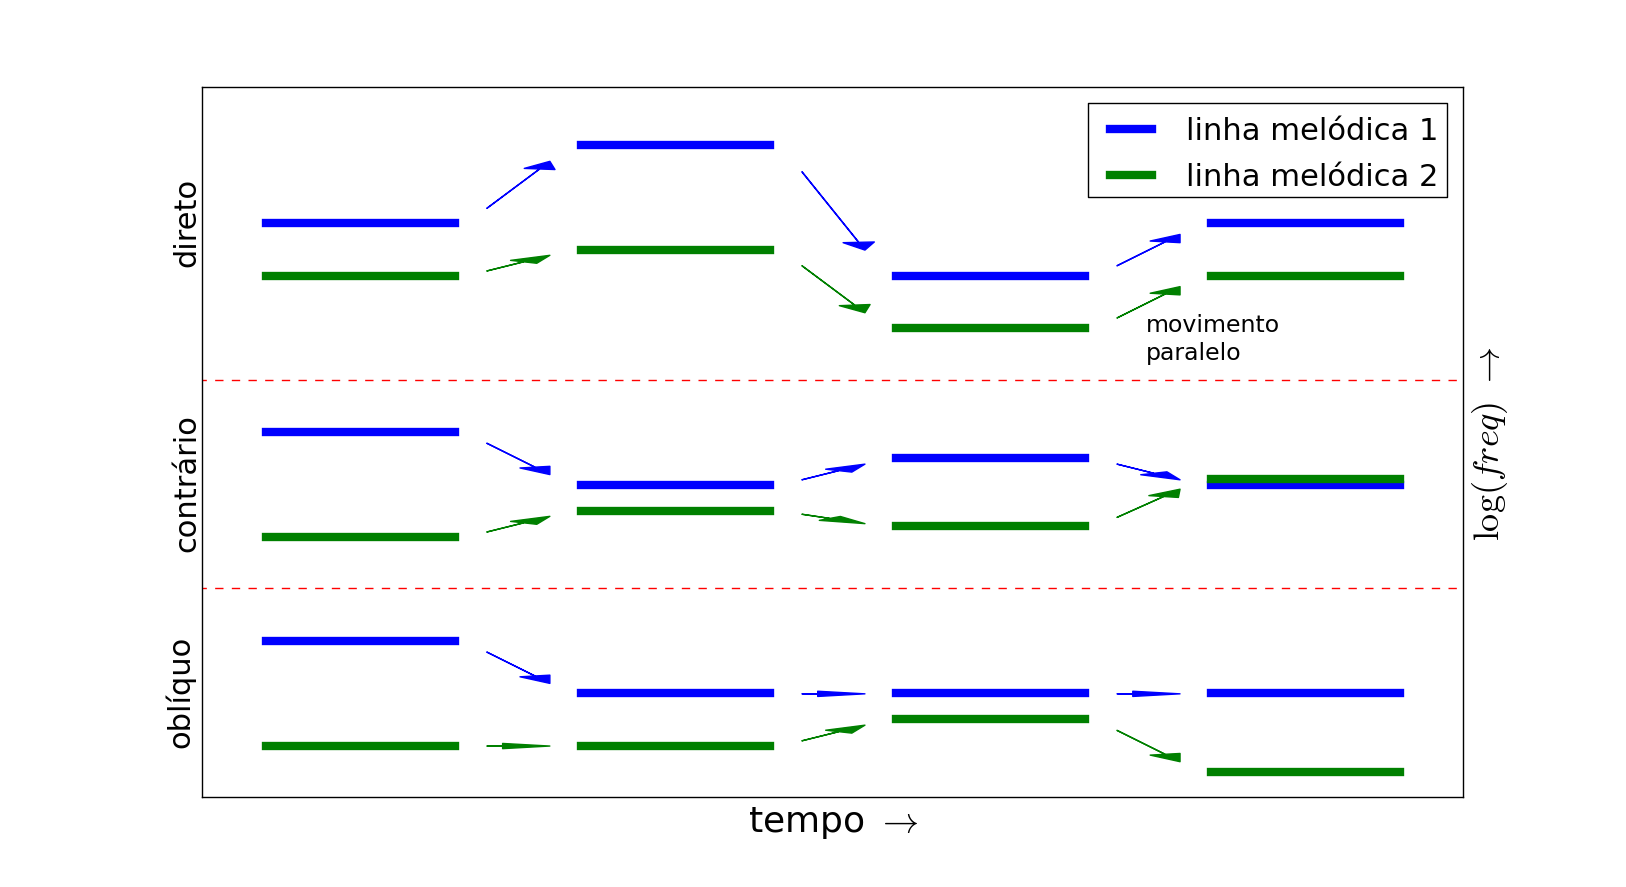
\includegraphics[width=\textwidth]{figuras/movContraponto}
    \caption{Movimentos diferenciados pelo contraponto com vistas a preservar a independência entre as vozes. 3 tipos de movimentos: direto, contrário e oblíquo, categorizam as possibilidades. O movimento paralelo é um tipo de movimento direto.}
        \label{fig:movContraponto}
\end{figure}



O propósito do contraponto é conduzir as vozes 
de forma que soem independentes. Cruciais para isso
são as movimentações relativas, das vozes duas a duas,
categorizadas em: movimento direto, oblíquo e contrário
conforme a figura~\ref{fig:movContraponto}. O movimento paralelo
é um movimento oblíquo.
A regra de ouro é cuidar que os movimentos diretos
não terminem em consonância perfeita. O movimento paralelo
deve só ocorrer entre consonâncias imperfeitas e não mais
do que três vezes consecutivas. As dissonâncias podem
ser não admitidas ou usadas seguidas 
e precedidas de consonâncias em graus conjuntos, i.e. notas vizinhas na escala.
Os movimentos que levam a nota a uma vizinha soam mais coerentes.
Na presença de 3 ou mais vozes,
a importância melódica recai sobre as vozes mais aguda e mais grave, neta ordem.\cite{Fux,Tragtenberg,SchoenbergContra}

Estas regras foram usadas na montagem \emph{Conta ponto}, o código está no Apêndice~\ref{ap:conta} e disponível online junto à \massa.


\subsection{Ritmo}\label{subsec:ritmo}
A noção rítmica é dependente de eventos separados por durações.\cite{Lacerda} Estes eventos podem ser ouvidos individualmente se separados
por ao menos $50-63ms$. Para que a separação entre eles possa ser apreciada como duração, ela deve ser maior,
por volta de $100ms$.\cite{microsound} Pode-se sumarizar 
a transição
de durações ouvidas como alturas para a apreciação em ritmo da seguinte forma:\cite{Alfaix, microsound}

\begin{table}[htpq!]
\tiny
\centering
\caption{Transição das durações ouvidas individualmente para alturas.}
\begin{tabular}{  l | r r r r   r r r    r r r || r r || r r r r r r }
\hline
           & \multicolumn{10}{c}{$\underleftarrow{\text{\bf zona de percepção de durações em ritmo}}$} & \multicolumn{2}{c}{transição} & \multicolumn{3}{c}{-} \\
duração (s) & {\bf ...}     & {\bf 32,}     & {\bf 16,}   & {\bf 8,}  & {\bf 4,}   & {\bf 2,}   & {\bf 1,}   & {\bf 1/2,} & {\bf 1/4,} & {\bf 1/8,} & $\frac{1}{16}=62,5ms$ , & $\frac{1}{20}=50ms$ & {\color{Gray} 1/40} & {\color{Gray} 1/80  } & {\color{Gray} 1/160 } & {\color{Gray} 1/320 } & {\color{Gray} 1/640 } & {\color{Gray} ... } \\
frequência (Hz) & {\color{Gray} ...} & {\color{Gray} 1/32,}   & {\color{Gray} 1/16,} & {\color{Gray} 1/8,} & {\color{Gray} 1/4,} & {\color{Gray} 1/2,} &  {\color{Gray} 1,}  & {\color{Gray} 2,}   & {\color{Gray} 4,}   & {\color{Gray} 8,}    & 16,  & 20   & {\bf 40}   & {\bf 80}   & {\bf 160}   & {\bf 320}   & {\bf 640}   & {\bf ...} \\
           & \multicolumn{10}{c}{ - } & \multicolumn{2}{c}{transição} & \multicolumn{6}{c}{$\overrightarrow{\text{\bf zona de percepção de durações em altura}}$} \\
\hline
\end{tabular}
\label{tab:duracoes}
\end{table}

A banda de durações marcada como transição está minimizada pois os limites não são bem definidos: a duração em que se começa a perceber uma frequência fundamental ou uma separação entre as ocorrências é dependente da pessoa e de características do som.\cite{microsound,Roederer}

A métrica rítmica costuma se basear em uma duração básica chamada pulso. O pulso tipicamente
compreende durações entre $0.25-1.5s$ (respectivamente $240$ e $40BPM$). Na educação musical e estudos cognitivistas,
costuma-se associar esta gama de frequências de pulsação às durações entre batidas 
do coração, da inspiração/expiração ou entre os passos ao caminhar.\cite{Lacerda,Roederer}

O pulso é subdividido em partes iguais e também é 
repetido sequencialmente. Estas relações (de divisão e de concatenação) costumam
seguir relações de números inteiros de baixa ordem
\footnote{Em ordem crescente de ocorrência na música
escrita e étnica,
as divisões do pulso musical e seus agrupamentos
sequenciais no tempo são: 2, 4 e 8, depois 3, 6 (dois grupos de 3 ou 3 grupos de 2) e 9 e 12 (3 e 4 grupos de 3). Por 
último os primos 5 e 7, completando 1-9 e 12.
Outras métricas são menos usuais, como divisões ou agrupamentos em 13, 17, etc, e são incidentes principalmente em contextos de música experimental e erudita do século XX e XXI. Por mais complexas que pareçam, as métricas costumam ser composições e decomposições de 1-9 partes iguais.\cite{Gramani,Roederer}.}.
Uma exposição esquemática está na figura~\ref{fig:pulsoSubAgl}.

\begin{figure}[h!]
    \centering
        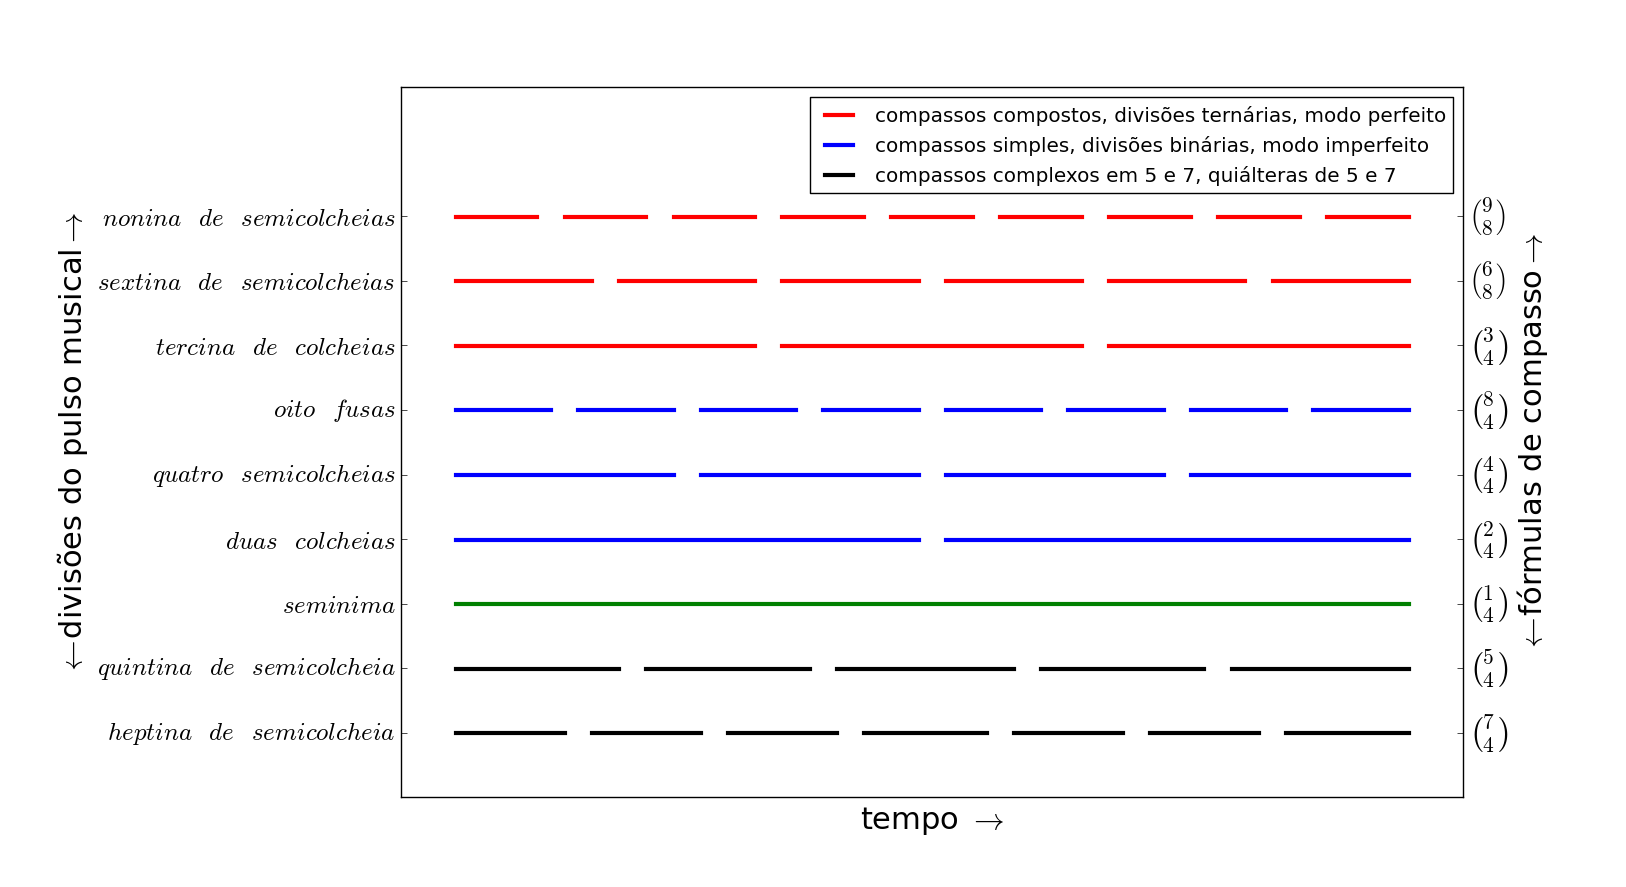
\includegraphics[width=\textwidth]{figuras/metricaMusical}
    \caption{Divisões e aglomerações do pulso musical para estabelecimento de métrica. Ao lado esquerdo estão as divisões da semínima estabelecida como pulso. Ao lado direito, fórmulas de compasso que especificam as mesmas métricas, mas na escala das aglomerações do pulso musical.}
        \label{fig:pulsoSubAgl}
\end{figure}

As relações duais (compassos simples e divisões binárias) costumam ocorrer em ritmos de dança
e ocasiões festivas, e são chamadas imperfeitas. As relações ternárias
incidem mais na música ritualística e relacionada ao sagrado
e são ditas perfeitas.

As unidades mais fortes (acentuadas) são as que consistem nas 'cabeças das divisões'. A cabeça de uma unidade é a primeira parte da subdivisão. Nas divisões binárias (2, 4 e 8 dos casos considerados),
as unidades consideradas fortes se revezam com as fracas
(e.g. a divisão em 4 é forte, fraco, meio-forte, fraco).
Nas divisões ternárias (3, 6 e 9)
à unidade forte (primeira) se sucedem 2 unidades fracas (e.g. a divisão em 3 é forte, fraco fraco)\footnote{A divisão em 6 é considerada composta
 mas pode ocorrer também como uma divisão binária.
 Uma divisão binária que sofre então uma divisão ternária
 resulta em duas unidades divididas em três unidades cada: forte (subdividido em forte fraco, fraco) e fraco (subdividido em forte, fraco, fraco).
A outra forma de ocorrer a divisão em 6 é através de 
uma divisão ternária que sofre então uma divisão binária, resultando em:
uma unidade forte (subdividido em forte e fraco) e duas unidades fracas (subdivididas em forte e fraco cada).}.

A acentuação em tempo fraco é o contratempo, as notas iniciadas em tempo fraco e cuja duração se prolonga sobre tempos fortes são as síncopas.

As notas podem ocorrer dentro e fora destas divisões da \emph{'métrica musical'}. Nos casos mais comportados, as notas ocorrem exatamente nestas divisões, com maior incidência em ataques nos tempos fortes.
Em casos extremos, não se pode perceber a métrica.\cite{Roederer} Variações pequenas na grade ajudam a compor a interpretação musical e diferenças entre estilos.\cite{Cook}

Seja o pulso o nível $j=0$ de agrupamento, o nível $j=-1$ 
a primeira subdivisão do pulso, o nível $j=1$ a primeira algomeração dos pulsos e assim por diante. 

Desta forma, $P_i^j$ é a $i$-ésima unidade de 
pulsos no nível $j$ de agrupamento:
$P^0_{10}$ é o décimo pulso, $P^{1}_3$ é a terceira unidade de agrupamento de pulsos (é possivel que seja o terceiro compasso),
$P^{-1}_2$ é a segunda unidade da subdivisão do pulso.

Especial atenção para
os limites de $j$: as divisões do pulso são durações apreciáveis
como ritmo; além disso, as junções do pulso somam, no máximo
do escopo, uma música ou um conjunto coeso de músicas. Dito de outra forma: a duração de $P^{min(j)}_i$, $\forall \; i$,
é maior que $50ms$ e as durações somadas $\sum_{\forall i}P^{\text{máx}(j)}_i$
é menor do que alguns minutos ou, no máximo, poucas horas.


Cada nível $j$ possui alguns índices $i$. Sempre que $i$ possuir três valores diferentes
(ou múltiplo de três) índices há uma relação perfeita, 
quando é somente múltiplo dois, quatro ou oito índices há uma relação imperfeita, como na figura~\ref{fig:pulsoSubAgl}.


Qualquer unidade (nota), de uma
dada sequência musical que tenha métrica pode ser
univocamente assim especificada:

\begin{equation}
P^{ \{ j_k \} }_{ \{ i_{k} \}}
\end{equation}

em que $j_k$ é o nível de aglomeração e $i_k$ é a ordem
da unidade em si.

Como um exemplo, $P^{-1,0,1}_{3,2,2}$  é a terceira subdivisão $P^{-1}_3$ do segundo
pulso $P^0_2$ do segundo aglomerado de pulsos $P^1_2$.
Cada unidade ou conjunto de unidades $P_i^j$ pode ser associada a uma sequência de amostras temporais $T_i$ que forma uma nota musical. 

A montagem \emph{Poli Hit Mia} utiliza as diferentes métricas e está no Apêndice~\ref{ap:poli}, disponível online como parte da \massa.

\subsection{Repetição e variação: motivos e unidades maiores}\label{subsec:motivos}
Dadas as estruturas musicais básicas tanto frequenciais (acordes e escalas) quanto 
rítmicas (divisões e aglomerações simples, compostas e complexas), é 
natural apresentar estas estruturas de forma que tenham coesão e sentido.\cite{Boulez}
Para tal, é fundamental o conceito de arcos: partindo de algum lugar e voltando, forma-se um arco. 
A audição de linhas melódicas e harmônicas é permeada de arcos musicais pela natureza cognitiva
da escuta musical. Pode-se considerar a nota o menor arco, cada motivo e melodia também um arco.
Cada tempo e cada subdivisão, cada compasso e secção da música, constitui um arco próprio.
Uma música, cujos arcos não apresentam consistência entre si, pode ser compreendida como uma música sem coesão.
A sensação de coerência provém, em grande parte, do tratamento hábil dos arcos de uma peça.

Os arcos músicais são estruturas abstratas e passíveis de operações básicas. Um arco espectral, como um
acorde, pode ser invertido, ampliado, permutado, por exemplo. Os arcos temporais, como uma melodia, um motivo, um compasso ou
uma nota, são igualmente passíveis de variações. Lembrando que $S_j=\left\{s_j=T_i^j=\{t_i^{j}\}_0^{\Lambda_j-1}\right\}_0^{H-1}$ é uma
sequência de $H$ eventos musicais $s_j$, cada evento com suas $\Lambda_j$ amostras $t_i^j$ (veja no início desta seção~\ref{notasMusica}), as técnicas básicas podem ser descritas assim:

\begin{itemize}
    \item A translação temporal é o deslocamento $\delta$ do material para um outro instante $\Gamma'=\Gamma + \delta$ da música. É uma variação do material com modificação na localização no decorrer da música: $\left\{s_j'\right\}=\left\{s_j^{\Gamma'}\right\}=\left\{s_j^{\Gamma+\delta}\right\}$ onde $\Gamma$ é a duração entre o começo da peça (ou trecho considerado) e o primeiro evento $s_0$ da estrutura $S_j$ original. Observe que $\delta$ é o deslocamento no tempo.
    \item A dilatação ou contração temporal é a alteração da duração de cada arco por um fator $\mu\,:\; s_j'^{\Delta}=s_j^{\mu_j . \Delta}$. Possivelmente, $\mu_j=\mu$ constante.
    \item Reversão temporal consiste em gerar uma sequência com os elementos em ordem invertida da sequência original $S_j$, assim: $S_j'=\left\{s_j'\right\}_0^{H-1}=\left\{s_{(H-j-1)}\right\}_0^{H-1}$.
    \item A inversão intervalar é a inversão do sentido dos intervalos percorridos pelo material. A inversão é estrita se o número de semitons esteja sendo usado como referência para a operação: $S_j'=\{s_j'\}_0^{H-1}=\left\{s_j^{-\varepsilon_j . f_0}\right\}$, onde $\varepsilon_j$ é o fator entre a frequência do evento $s_j$ e a frequência de $s_0$. A inversão é tonal caso as distâncias sejam consideradas em termos de números de graus da escala $E_k$: $S_j'=\{s_j'\}_0^{H-1}=\left\{s_j^{-\varepsilon^{\left(e_{\left(j_e\right)}\right)} . f_0}\right\}_0^{H-1}$ onde $j_e=e_{j}^{inv}$ é o índice $k=j_e$ em $E_k$ da nota do evento $s_j$.
    \item A inserção e remoção de materiais na estrutura $S_j$ pode ser ornamental ou estruturante: $S_j'=\{s_j'\}=\{s_j \text{ se condição A, caso contrário } r_j\}$, para qualquer material musical $r_j$, incluindo o instante vazio. Elementos de $R_j$ podem ser inseridos no começo, como uma prefixo de $S_j$, ao final, como um sufixo, ou no meio, dividindo $S_j$ ou fazendo dele o prefixo e o sufixo. Os dois materiais podem se misturar das formas mais diversas.
    \item Modificações de articulação, instrumentação e espacialização $s_j'=s_j^{*_j}$, com $*_j$ a nova característica incorporada pelo elemento $s_j'$.
    \item Acompanhamento, tanto a instrumentação quanto as linhas melódicas que presentes na ocorrência de $S_j$ podem sofrer modificações e ser considerada uma variação de $S_j$ em si.
\end{itemize}

Com estes procedimentos, outros são derivados: o retrógrado do inverso, uma contração temporal com um sufixo externo, etc.
A estruturas musicais ressoam mentalmente devido à própria natureza do pensamento.
As ideias dizem respeito a objetos/contextos. Em suas várias facetas,
uma ideia lida com o mesmo número de elementos e aspectos conectivos entre eles.
A música, através de sintonia com estas estruturas mentais, suscita impressões. É, assim, desencadeado
todo um processo de ressonância mental e cortical responsável pelos sentimentos, lembranças e imaginações
típicas de uma audição musical atenta. Esta atividade neurológica contribui para a terapia
músical, conhecida pela utilidade em casos de depressão e dano neurológico. Considera-se que as regiões do cérebro responsáveis pelo processamento auditivo são também usadas para outras atividades, incluindo linguísticas e matemáticas.\cite{Sacks,Roederer}

Como princípios gerais que orientam a criação de novos materiais musicais, utiliza-se estruturas paradigmáticas. Uma delas, central, é o dipolo tensão/relaxamento. Relaciona-se com este dipolo, cada outro dipolo tradicional: tônica/dominante, repetição/variação, consonância/dissonância, coerência/rompimento, simetria/assimetria, chegada/saída, perto/longe, parado/em movimento, etc. Já as relações ternárias tendem a se relacionar com o circular e a unificação.
A subseção seguinte é dedicada aos arcos direcionais e, 
no seguinte, os arcos cíclicos.

\subsection{Estruturas direcionais}\label{subsec:dir}


Os arcos podem ser decompostos em duas sequências convergentes: 
uma que atinge o ápice, e 
outra que, de forma paradigmática, volta do ápice à região de partida. Este ápice é chamado de clímax pela teoria musical tradicional. Distingue-se entre arcos cujos clímax estão: no começo, no meio, no final, na primeira metade e na segunda metade da duração considerada. Estas estruturas estão na figura~\ref{fig:climax}. O parâmetro que varia pode não existir, no caso o arco consiste somente em uma estrutura de referência.\cite{Schoenberg}

\begin{figure}[h!]
    \centering
        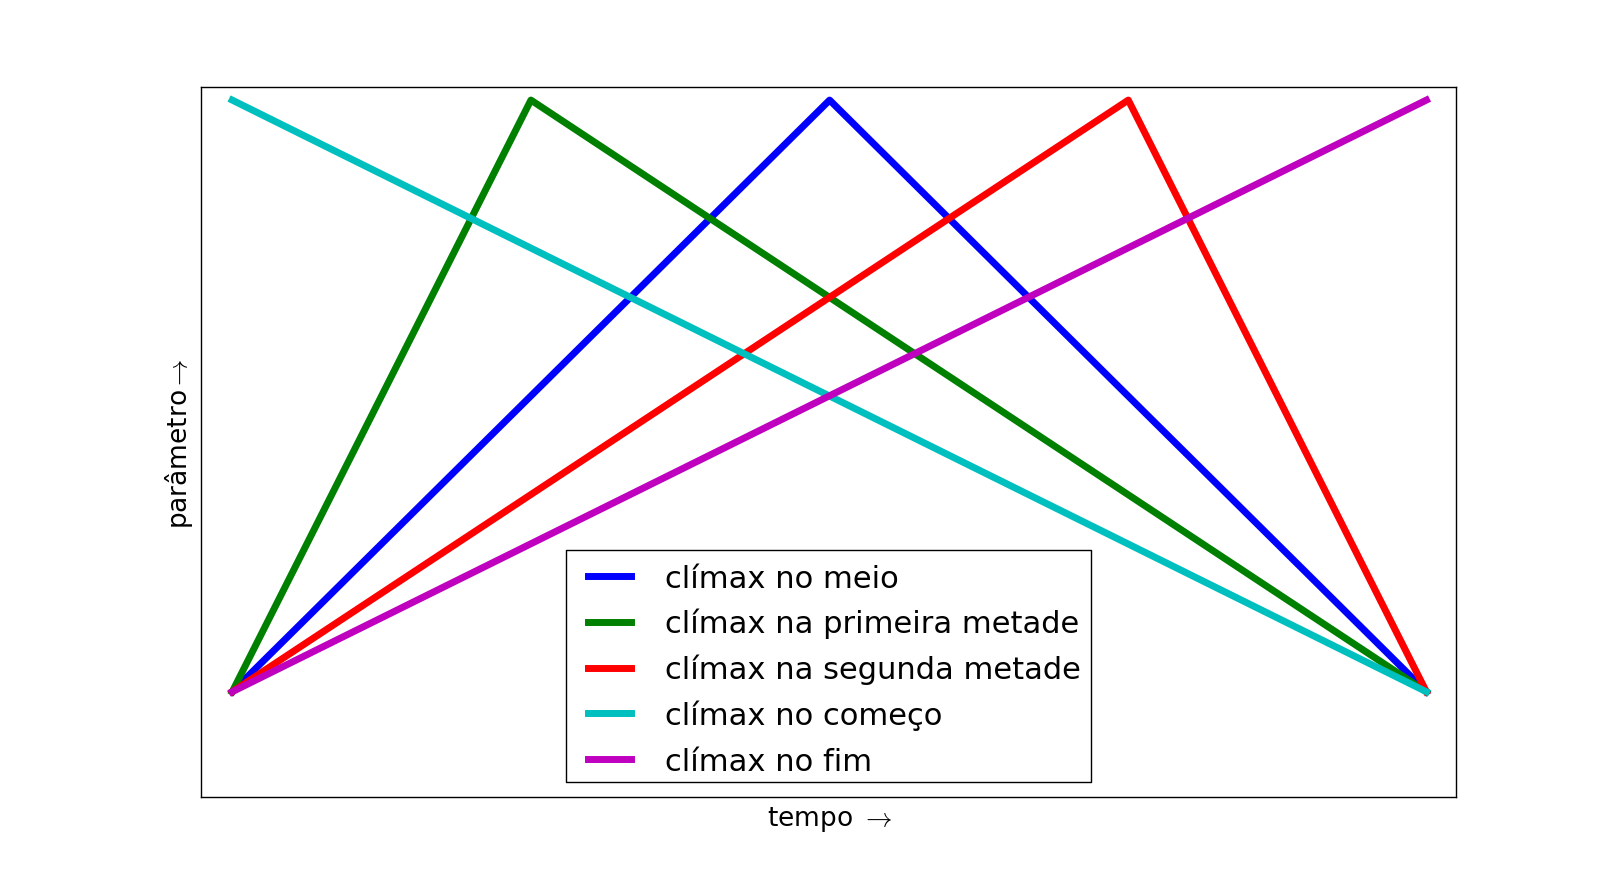
\includegraphics[width=\textwidth]{figuras/climax}
    \caption{Distinções canônicas do clímax musical em uma melodia e outros domínios. As possibilidades diferenciadas são: clímax no começo, clímax na primeira metade, clímax no meio, clímax na segunda metade, clímax no fim. Não está especificado o eixo das ordenadas pois pode não haver variação paramétrica real, neste caso a estrutura é uma referência.}
        \label{fig:climax}
\end{figure}


Seja $S_i=\{s_i\}_0^{H-1}$ uma sequência crescente. A sequência 
$R_i=\{r_i\}_0^{2H -2}=\left\{s_{(H-1-|H-1-i|)}\right\}_0^{2H-2}$ 
é uma sequência que apresenta simetria especular perfeita, i.e. a segunda metade é uma versão espelhada da primeira. Segundo conceitos musicais, o clímax está exatamente no meio da sequência. Pode-se modificar isso com a substituição por sequências de tamanhos diferentes. Toda a teoria matemática de sequências, já estabelecida e ensinada corriqueiramente em cursos de cálculo III, pode ser utilizada para geração destes arcos.\cite{Guidorizzo,Schoenberg}
Teoricamente, estas sequências aplicadas desta forma
a qualquer característica dos eventos musicais produz arcos,
pois implicam no afastamento e retorno de uma parametrização inicial. 
Assim, é possível para uma mesma sequência de eventos possuir um número de arcos distintos, com tamanhos e clímax diferentes. Este é um recurso
interessante e útil e a correlação dos arcos resulta na coerência da escuta.\cite{Salzer}

A montagem sonora \emph{Dirracional} expõe estes arcos em estruturas direcionais. Seu código está no Apêndice~\ref{ap:dirracional} e disponível online como parte da \massa.\cite{MASSA}

\subsection{Estruturas cíclicas}\label{estCic}

O entendimento filosófico de que o pensamento humano é fundamentado
na percepção de semelhanças e diferenças dentre os estímulos
e objetos coloca
as simetrias no cerne do processo cognitivo.\cite{Deleuze}
Matematicamente,
as simetrias são grupos algébricos e um grupo finito
é sempre isomorfo a um grupo de permutações. 
Pode-se dizer que
as permutações representam quaisquer simetrias em um sistema finito.
Na música, as permutações são ubíquas
e estão presentes em técnicas, o que confirma seu papel central.
A aplicação sucessiva das permutações gera arcos cíclicos.\cite{change,Zamacois,permMusic}
A esta abordagem foram dedicados dois trabalhos acadêmicos para geração de estruturas musicais.\cite{figgusOriginal, figgusEspacializacao}

Qualquer conjunto de permutações pode ser utilizado como gerador de grupos algébricos.\cite{permMusic} As propriedades que definem um grupo $G$ são:

\begin{equation}\label{eq:groups}
\begin{split}
\forall \;\; p_1,p_2 \in G \Rightarrow\quad\quad\quad\;\; p_1 \bullet p_2 & = p_3 \in G  \quad\quad\quad\;\;\;\text{(propriedade de fechamento)} \\
\forall \;\; p_1,p_2,p_3 \in G \Rightarrow\quad (p_1\bullet p_2)\bullet p_3 & = p_1\bullet (p_2\bullet p_3)\quad\;  \text{(propriedade da associatividade)} \\
\exists \;\; e \in G :\quad\quad\quad\quad\; p \bullet e & = e \bullet p \;\;\;\; \forall p \in G  \quad \text{(existência do elemento neutro)} \\
\forall \;\; p \in G, \;\exists\; p^{-1} :\quad\quad\quad\;  p\bullet p^{-1} & =p^{-1}\bullet p = e  \quad\quad\;\text{(existência do inverso)}
\end{split}
\end{equation}


Da primeira propriedade conclui-se que toda permutação pode ser operada com outra permutação. De fato, pode-se aplicar uma permutação $p_1$, depois outra $p_2$ e, se comparadas as ordenações inicial e final, há uma permutação $p_3$.

Todo elemento $p$ operado consigo mesmo um número suficiente de vezes $n$ atinge o elemento neutro $p^n=e$, caso contrário o grupo seria infinito (gerado por $p$). O menor $n\;:\;p^n=e$ é chamado de ordem do elemento. Assim, uma permutação finita $p$ aplicada sucessivamente atinge a ordenação inicial dos elementos, formando um ciclo. Este ciclo, se utilizado para parametros de notas musicais, implica em um arco musical cíclico.

Estes arcos podem ser efetuados pelo uso conjunto de diferentes permutações. Como exemplo
histórico, a tradição chamada \emph{change ringing} concebe música através de sinos tocados um após o outro e então tocados novamente, mas em uma ordem diferente. Este processo se repete até que se atinja a ordenação inicial. O conjunto de ordenações diferentes percorridas é um \emph{peal}. A tabela~\ref{tab:change} representa um \emph{peal} tradicional de 3 sinos (1, 2 e 3) que explora todas as suas ordenações. Cada linha apresenta uma ordenação dos sinos a ser tocada. As permutações estão entre as linhas.
Neste caso, a estrutura musical consiste em permutações propriamente ditas e algumas permutações diferentes operam para o comportamento cíclico. 

\begin{table}[htpq!]
\centering
\caption{Change Ringing: \emph{Peal} (padrão) com 3 sinos. As permutações estão entre as ordenações. Cada linha é uma ordednação dos sinos, cada ordenaçao é tocada, uma linha por vez.}
\begin{tabular}{l c r}
\textcolor{red}{1} & \textcolor{blue}{2} & \textcolor{green}{3} \\
\textcolor{blue}{2} & \textcolor{red}{1} & \textcolor{green}{3} \\
\textcolor{blue}{2} & \textcolor{green}{3} & \textcolor{red}{1} \\
\textcolor{green}{3} & \textcolor{blue}{2} & \textcolor{red}{1} \\
\textcolor{green}{3} & \textcolor{red}{1} & \textcolor{blue}{2} \\
\textcolor{red}{1} & \textcolor{green}{3} & \textcolor{blue}{2} \\
\textcolor{red}{1} & \textcolor{blue}{2} & \textcolor{green}{3}
\end{tabular}
\label{tab:change}
\end{table}


A utilização de permutações na música pode ser resumida da seguinte forma:
seja $L_i$ uma sequência de eventos musicais (e.g. notas) e $p$ uma permutação.
$L_i'=p(L_i)$ consiste nos mesmos elementos de $L_i$ mas em ordem diferente.
As permutações podem ser escritas em duas notações: cíclica ou natural. 
A notação natural consiste na ordem dos índices 
resultante da permutação. Assim,
convencionada a ordenação original dada pela sequência de seus índices $[0\;1\;2\;3\;4\;5\;...]$ a permutação é notada pela sequência que produz (ex. $[1\;3\;7\;0\;...]$). Na notação cíclica, a permutação é a troca de um elemento pelo
da frente, e o último pelo primeiro.

Não é necessário permutar os elementos de $L_i$, mas somente
alguma ou algumas de suas características. Assim, seja $p^f$ uma permutação 
nas frequências e $L_i$ uma sequência de notas básicas como expostas
ao final de~\ref{notaBasica}. A nova sequência $L_i'=p^f(L_i)$ consiste nas mesmas
notas musicais, na mesma ordem e com as mesmas características, com as frequências fundamentais permutadas segundo o padrão que $p^f$ apresenta.

Duas sutilezas deste procedimento.
1) A permutação $p$ não precisa envolver todos os elementos de $L_i$, i.e. ela
pode operar em subconjuntos de $L_i$. 2) Nem todos os elementos $l_i$ precisam ser executados a cada consulta de estado realizada.
Para exemplificar, seja $L_i$ 
uma sequência de notas musicais $l_i$. 
Se $i$ vai de $0$ a $n$, e $n>4$, a cada compasso
de $4$ notas pode-se executar as primeiras $4$ notas. As outras notas de
$L_i$ podem incidir nos compassos em que as permutações aloquem
estas notas para as primeiras quatro notas de $L_i$.

Cada uma destas permutações
$p_i$ possui, ao menos, segundo a exposição acima: dimensões das notas em que opera (frequência, duração, \emph{fades}, intensidade, etc) e período de incidência (a cada quantas consultas é aplicada a permutação). Na realização das notas de $L_i$, uma forma fácil e coerente é executar as primeiras $n$ notas\footnote{A execução de notas disjuntas de $L_i$ equivale a modificar a permutação e executar as primeiras notas.}.

No Apêndice~\ref{cap:FIGGUScode} apontada a implementação computacional disponibilizada em.\cite{MASSA,figgusOriginal,figgusEspacializacao}

\subsection{Idioma musical?}

Existem diversas empreitadas que se propõem a modelar e explorar entendimentos
sobre a 'linguagem musical', a 'linguística aplicada à música' ou ainda
para discernimento entre 
o que seriam diferentes
`idiomas musicais'.\cite{Lerdahl, Harmonia, Salzer,Alfaix}
De forma simples, um idioma musical é fruto da escolha de materiais básicos e
repetição de elementos e da repetição de relações entre elementos presentes no decorrer da música. Nestas questões, as dicotomias são salientes,
como explicadas na subseção~\ref{subsec:motivos}: repetição e variação, relaxamento e tensão, equilíbrio e desequilíbrio, consonância e dissonância, etc. 

\subsection{Usos musicais}\label{subsec:usosmusicais3}

Primeiro, a nota básica foi definida e caracterizada em termos
claros e quantitativos (seção~\ref{sec:notaDisc}). Em seguida, a composição interna da nota foi abordada, e compreendidas as transições internas e tratamentos imediatos (seção~\ref{varInternas}). Por fim, esta presente seção dedica-se a organizar estas notas em música.
A gama de recursos e a consequênte infinidade de possibilidades de resultados
é situação típica e cara às artes.\cite{Harmonia,Webern}

Existem estudos para cada recurso apresentado. Por exemplo, pode-se obter as harmonias triádicas 'sujas' (com notas não pertencentes à tríade) através de sobreposições de quartas justas. Outro exemplo interessante é a presença simultânea de ritmos em diferentes métricas, constituindo o que chama-se de \emph{polirritmia}. A montagem musical \emph{Poli-hit mia} explora estas métricas simultâneas através de trem de impulsos convoluídos com as notas que compõem cada linha. Seu código está no Apêndice~\ref{ap:poli} e disponível online como parte da \massa.

As escalas microtonais são importantes na música do século XX~\cite{microtonalidade} e possuem resultados muito marcantes, como os quartos de tom na música indiana. A sequência musical \emph{MicroTom} explora estes recursos, incluindo melodias microtonais e harmonias microtonais com várias notas em um âmbito de alturas bastante reduzido. Seu código está no Apêndice~\ref{ap:micro} e disponível online como parte da \massa.

Como também apontado na subseção~\ref{subsec:mus2}, os vínculos entre parâmetros são formas poderosas de se obter peças e montagens musicais. O número de notas permutadas pode variar no decorrer da música, revelando vínculo com a duração da peça. As harmonias podem constituir-se triádicas (eqs.~\ref{triades}) com notas replicadas em várias oitavas e mais numerosas quanto menor a profundidade e frequência de vibratos (eqs.~\ref{vbrGamma},~\ref{vbrAux},~\ref{vbrF},~\ref{vbrGamma2},~\ref{vbrT}), dentre outras incontáveis possibilidades.

As simetrias apresentadas nas divisões da oitava (eqs.~\ref{escSim}) e as simetrias apresentadas através das permutações (tabela~\ref{tab:change} e eqs.~\ref{eq:groups}) podem ser usadas em conjunto. Nas peças \emph{3 trios} esta associação é feita de forma sistemática para possibilitar uma audição a ela dedicada. Esta é uma peça instrumental e não consta dentre os códigos dos Apêndices e da \massa.\cite{3Trios}

O \emph{PPEPPS} (Pure Python EP: Projeto Solvente) é um EP sintetizado com os recursos apresentados neste trabalho. Com pouca parametrização, o programa gera músicas inteiras, permitindo a composição de músicas e conjuntos de músicas com facilidade. Através de poucas linhas de código e, pela execução, pode-se obter uma pasta com as músicas. Esta facilidade e entrega tecnológica abre possibilidades estéticas, de compartilhamento e educacionais.


